\def\OptimizaTikZ{1}

%%%%%%%%%%%%%%%%%%%%%%%%%%%%%%%%%%%%%%%%%%%%%%%%%%%%%%%%%%%%%%%%%%%%%%%%
% Plantilla TFG/TFM
% Escuela Politécnica Superior de la Universidad de Alicante
% Realizado por: Jose Manuel Requena Plens
% Contacto: info@jmrplens.com / Telegram:@jmrplens
%%%%%%%%%%%%%%%%%%%%%%%%%%%%%%%%%%%%%%%%%%%%%%%%%%%%%%%%%%%%%%%%%%%%%%%%

%%%%%%%%%%%%%%%%%%%%%%%%
% FORMATO DEL DOCUMENTO
%%%%%%%%%%%%%%%%%%%%%%%%
% scrbook es la clase de documento
% Si se desea que no haya página en blanco entre capítulos añadir "openany" en los parámetros de la clase. Sino siempre los capítulos empezarán en página impar.
\documentclass[a4paper,11pt,titlepage]{scrbook}
\KOMAoption{toc}{bib,chapterentryfill} % Opciones del índice
\usepackage{scrhack} % Previene algunos errores
% Paquete de formato para scrbook. Con marcas, linea-separador superior e inferior
\usepackage[automark,headsepline,footsepline]{scrlayer-scrpage}
\clearpairofpagestyles		% Borra los estilos por defecto
%%
% Formato y contenido de la información de cabecera y pie de página
%%
% Información de capítulo en cabecera e interno
\ihead{{\color{gray30}\scshape\small\headmark}}	
% Número de página en cabecera y externo
\ohead{\normalfont\pagemark} 
% Número de página en pie de página y externo. Sólo en páginas sin cabecera
\ofoot[\normalfont\pagemark]{}
%% 		
% Edición del contenido de las distintas partes de la cabecera
%%
\renewcommand{\chaptermark}[1]{\markboth{#1}{}} % Capítulo (Solo texto)
\renewcommand{\sectionmark}[1]{\markright{\thesection. #1}} % Sección (Número y texto)
\setkomafont{pagenumber}{} % Número de página (Sin nada añadido)

% Añade al índice y numera hasta la profundidad 4.
% 1:section,2:subsection,3:subsubsection,4:paragraph
\setcounter{tocdepth}{4}
\setcounter{secnumdepth}{4}
% Muestra una regla para comprobar el formato de las páginas
%\usepackage[type=upperleft,showframe,marklength=8mm]{fgruler}
% MÁRGENES DE LAS PÁGINAS
\usepackage[
  inner	=	3.0cm, % Margen interior
  outer	=	2.5cm, % Margen exterior
  top	=	2.5cm, % Margen superior
  bottom=	2.5cm, % Margen inferior
  includeheadfoot, % Incluye cabecera y pie de página en los márgenes
]{geometry}
% Valor de interlineado
\renewcommand{\baselinestretch}{1.0} % 1 línea de interlineado
% Para poder generar páginas horizontales
\usepackage{lscape}
% Ancho de la zona para comentarios en el margen. (modificado para todonotes)
\setlength{\marginparwidth}{1.9cm}

%%%%%%%%%%%%%%%%%%%%%%%%
% BIBLIOGRAFÍA
%%%%%%%%%%%%%%%%%%%%%%%%
\usepackage{apacite} % NORMA APA
\usepackage{natbib}
\usepackage{breakcites}

%%%%%%%%%%%%%%%%%%%%%%%%
% DOCUMENTO EN ESPAÑOL
%%%%%%%%%%%%%%%%%%%%%%%%
\usepackage[base]{babel}
\usepackage{polyglossia}
\setdefaultlanguage{spanish}

\addto\captionsspanish{%
	\renewcommand{\listtablename}{Índice de tablas} 
	\renewcommand{\tablename}{Tabla}
	\renewcommand{\lstlistingname}{Código}
	\renewcommand{\lstlistlistingname}{Índice de \lstlistingname s}
	\renewcommand{\glossaryname}{Glosario}
	\renewcommand{\acronymname}{Acrónimos}
	\renewcommand{\bibname}{Bibliografía}%
}

%%%%%%%%%%%%%%%%%%%%%%%% 
% COLORES
%%%%%%%%%%%%%%%%%%%%%%%% 
% Biblioteca de colores
\usepackage{color}
\usepackage[dvipsnames]{xcolor}
% Otros colores definidos por el usuario
\definecolor{gray97}{gray}{.97}
\definecolor{gray75}{gray}{.75}
\definecolor{gray45}{gray}{.45}
\definecolor{gray30}{gray}{.30}

%%%%%%%%%%%%%%%%%%%%%%%%
% TABLAS
%%%%%%%%%%%%%%%%%%%%%%%%
% Paquetes para tablas
\usepackage{longtable,array}

\newcolumntype{L}[1]{>{\raggedright\let\newline\\\arraybackslash\hspace{0pt}}m{#1}}

\usepackage{tikz,tikzpagenodes}

\usetikzlibrary{tikzmark,calc,shapes.geometric,arrows,backgrounds,shadings,shapes.arrows,shapes.symbols,shadows,positioning,fit,automata,patterns,intersections}

%%%%%%%%%%%%%%%%%%%%%%%% 
% FIGURAS, TABLAS, ETC 
%%%%%%%%%%%%%%%%%%%%%%%% 
\usepackage{subcaption} % Para poder realizar subfiguras
\usepackage{caption} % Para aumentar las opciones de diseño
% Nombres de figuras, tablas, etc, en negrita la numeración, todo con letra small
\captionsetup{labelfont={bf,small},textfont=small}
% Paquete para modificar los espacios arriba y abajo de una figura o tabla
\usepackage{setspace}
% Define el espacio tanto arriba como abajo de las figuras, tablas
\setlength{\intextsep}{5mm}
% Para ajustar tamaños de texto de toda una tabla o grafica
% Uso: {\scalefont{0.8} \begin{...} \end{...} }
\usepackage{scalefnt}
% Redefine las tablas y figuras para eliminar el '.' entre la numeración y el texto
\renewcommand*{\figureformat}{\figurename~\thefigure}
\renewcommand*{\tableformat}{\tablename~\thetable}

%%%%%%%%%%%%%%%%%%%%%%%% 
% TEXTO
%%%%%%%%%%%%%%%%%%%%%%%%
% Paquete para poder modificar las fuente de texto
\usepackage{xltxtra}
% Cualquier tamaño de texto. Uso: {\fontsize{100pt}{120pt}\selectfont tutexto}
\usepackage{anyfontsize}
% Para modificar parametros del texto.
\usepackage{setspace}
% Paquete para posicionar bloques de texto
\usepackage{textpos}
% Paquete para realizar cajas de texto. 
% Uso: \begin{mdframed}[linecolor=red!100!black] tutexto \end{mdframed}
\usepackage{framed,mdframed}
% Para subrayar. Uso: \hlc[tucolor]{tutexto}
\newcommand{\hlc}[2][yellow]{ {\sethlcolor{#1} \hl{#2}} }

%%%%%%%%%%%%%%%%%%%%%%%% 
% OTROS
%%%%%%%%%%%%%%%%%%%%%%%%
% Para introducir url's con formato. Uso: \url{http://www.google.es}
\usepackage{url}
% Amplia muchas funciones graficas de latex
\usepackage{graphicx}
% Paquete que añade el hipervinculo en referencias dentro del documento, indice, etc
% Se define sin bordes alrededor. Uso: \ref{tulabel}
\usepackage[pdfborder={000}]{hyperref}
\usepackage{float}
\usepackage{placeins}
\usepackage{afterpage}
\usepackage{verbatim}
% Paquete para condicionales avanzados
\usepackage{xstring,xifthen}
% Paquete para realizar calculos en el código
\usepackage{calc}
% Para rotar tablas o figuras o su contenido
\usepackage{rotating} 
% Para incluir comentarios en el texto. El parámetro 'disable' oculta todas las notas.
% USO: \todo{tutexto}
\usepackage[textsize=tiny,spanish,shadow,textwidth=2cm]{todonotes}
%\reversemarginpar % Descomentar si se quiere todos los comentarios en el mismo lado
% Desactiva la exportación de los ToDo y Missingfigures como figuras

%%%%%%%%%%%%%%%%%%%%%%%% 
% GLOSARIOS
%%%%%%%%%%%%%%%%%%%%%%%%
\usepackage[acronym,nonumberlist,toc]{glossaries}
\usepackage{glossary-superragged}
\newglossarystyle{modsuper}{%
  \setglossarystyle{super}%
  \renewcommand{\glsgroupskip}{}
}
\renewcommand{\glsnamefont}[1]{\textbf{#1}}


%%%%%%%%%%%%%%%%%%%%%%%% 
% COMANDOS AÑADIDOS
%%%%%%%%%%%%%%%%%%%%%%%%
% Para mostrar la fecha actual (mes año) con \Hoy
\newcommand{\MES}{%
  \ifcase\month% 0
    \or Enero% 1
    \or Febrero% 2
    \or Marzo% 3
    \or Abril% 4
    \or Mayo% 5
    \or Junio% 6
    \or Julio% 7
    \or Agosto% 8
    \or Septiembre% 9
    \or Octubre% 10
    \or Noviembre% 11
    \or Diciembre% 12
  \fi}
\newcommand{\ANYO}{\number\year}
\newcommand{\Hoy}{\MES\ \ANYO}

%%%%%
% PARÁMETROS DE FORMATO DE CODIGOS
%%%%%
% Puedes editar los formatos para ajustarlos a tu gusto
%%%%%%%%%%%%%%%%%%%%%%%%%%%%%%%%%%%%%%%%%%%%%%%%%%%%%%%%%%%%%%%%%%%%%%%%
% Plantilla TFG/TFM
% Escuela Politécnica Superior de la Universidad de Alicante
% Realizado por: Jose Manuel Requena Plens
% Contacto: info@jmrplens.com / Telegram:@jmrplens
%%%%%%%%%%%%%%%%%%%%%%%%%%%%%%%%%%%%%%%%%%%%%%%%%%%%%%%%%%%%%%%%%%%%%%%%


%%%%%%%%%%%%%%%%%%%%%%%% 
% CÓDIGO. CONFIGURACIÓN. En el siguiente bloque están los estilos.
%%%%%%%%%%%%%%%%%%%%%%%%
% Paquete para mostrar código de matlab. En caja y lineas numeradas
\usepackage[framed,numbered]{matlab-prettifier}
% Paquete mostrar código de programación de distintos lenguajes
\usepackage{listings}
\lstset{ inputencoding=utf8,
extendedchars=true,
frame=single, % Caja donde se ubica el código
backgroundcolor=\color{gray97}, % Color del fondo de la caja
rulesepcolor=\color{black},
boxpos=c,
abovecaptionskip=-4pt,
aboveskip=12pt,
belowskip=0pt,
lineskip=0pt,
framerule=0pt,
framextopmargin=4pt,
framexbottommargin=4pt,
framexleftmargin=11pt,
framexrightmargin=0pt,
linewidth=\linewidth,
xleftmargin=\parindent,
framesep=0pt,
rulesep=.4pt,
stringstyle=\ttfamily,
showstringspaces = false,
showspaces = false,
showtabs = false,
columns=fullflexible,
basicstyle=\small\ttfamily,
commentstyle=\color{gray45},
keywordstyle=\bfseries,
tabsize=4,
numbers=left,
numbersep=1pt,
numberstyle=\tiny\ttfamily\color{gray75},
numberfirstline = false,
breaklines=true,
postbreak=\mbox{\textcolor{red}{$\hookrightarrow$}\space}, % Flecha al saltar de linea
prebreak=\mbox{\textcolor{red}{$\hookleftarrow$}\space}, % Flecha al saltar de linea
literate=
  {á}{{\'a}}1 {é}{{\'e}}1 {í}{{\'i}}1 {ó}{{\'o}}1 {ú}{{\'u}}1
  {Á}{{\'A}}1 {É}{{\'E}}1 {Í}{{\'I}}1 {Ó}{{\'O}}1 {Ú}{{\'U}}1
  {à}{{\`a}}1 {è}{{\`e}}1 {ì}{{\`i}}1 {ò}{{\`o}}1 {ù}{{\`u}}1
  {À}{{\`A}}1 {È}{{\'E}}1 {Ì}{{\`I}}1 {Ò}{{\`O}}1 {Ù}{{\`U}}1
  {ä}{{\"a}}1 {ë}{{\"e}}1 {ï}{{\"i}}1 {ö}{{\"o}}1 {ü}{{\"u}}1
  {Ä}{{\"A}}1 {Ë}{{\"E}}1 {Ï}{{\"I}}1 {Ö}{{\"O}}1 {Ü}{{\"U}}1
  {â}{{\^a}}1 {ê}{{\^e}}1 {î}{{\^i}}1 {ô}{{\^o}}1 {û}{{\^u}}1
  {Â}{{\^A}}1 {Ê}{{\^E}}1 {Î}{{\^I}}1 {Ô}{{\^O}}1 {Û}{{\^U}}1
  {œ}{{\oe}}1 {Œ}{{\OE}}1 {æ}{{\ae}}1 {Æ}{{\AE}}1 {ß}{{\ss}}1
  {ű}{{\H{u}}}1 {Ű}{{\H{U}}}1 {ő}{{\H{o}}}1 {Ő}{{\H{O}}}1
  {ç}{{\c c}}1 {Ç}{{\c C}}1 {ø}{{\o}}1 {å}{{\r a}}1 {Å}{{\r A}}1
  {€}{{\euro}}1 {£}{{\pounds}}1 {«}{{\guillemotleft}}1
  {»}{{\guillemotright}}1 {ñ}{{\~n}}1 {Ñ}{{\~N}}1 {¿}{{?`}}1,
  }

% Intenta no dividir los códigos en diferentes paginas si es posible
\lstnewenvironment{listing}[1][]
   {\lstset{#1}\pagebreak[0]}{\pagebreak[0]}

% Formato de títulos de los códigos
\DeclareCaptionFont{white}{\color{white}}
\DeclareCaptionFormat{listing}{\colorbox{gray}{\parbox{\textwidth - 2\fboxsep}{#1#2#3}}}
\captionsetup[lstlisting]{format=listing,labelfont=white,textfont=white,font= scriptsize}


%%%%%%%%%%%%%%%%%%%%%%%% 
% CÓDIGO. ESTILOS. Ajústalos a tu gusto
%%%%%%%%%%%%%%%%%%%%%%%%
\lstdefinestyle{Consola}
	{
	basicstyle=\scriptsize\bfseries\ttfamily,
	}
   
\lstdefinestyle{C}
	{
	basicstyle=\scriptsize,
	language=C,
	}
\lstdefinestyle{C-color}
	{
  	breaklines=true,
  	language=C,
  	basicstyle=\scriptsize,
  	keywordstyle=\bfseries\color{green!40!black},
  	commentstyle=\itshape\color{purple!40!black},
  	identifierstyle=\color{blue},
  	stringstyle=\color{orange},
    }
\lstdefinestyle{CSharp}
	{
	basicstyle=\scriptsize,
	language=[Sharp]C,
	escapeinside={(*@}{@*)},
	keywordstyle=\bfseries,
	}
\lstdefinestyle{CSharp-color}
	{
	basicstyle=\scriptsize,
	language=[Sharp]C,
	escapeinside={(*@}{@*)},
	commentstyle=\color{greencomments},
	keywordstyle=\color{bluekeywords}\bfseries,
	stringstyle=\color{redstrings},
	}
\lstdefinestyle{C++}
	{
	basicstyle=\scriptsize,
	language=C++,
 	}
 	
\lstdefinestyle{C++-color}
	{
  	breaklines=true,
  	language=C++,
  	basicstyle=\scriptsize,
  	keywordstyle=\bfseries\color{green!40!black},
  	commentstyle=\itshape\color{purple!40!black},
  	identifierstyle=\color{blue},
  	stringstyle=\color{orange},
    }
    
\lstdefinestyle{PHP}
	{
	basicstyle=\scriptsize,
	language=PHP,
	}
	
\lstdefinestyle{PHP-color}
	{
	basicstyle=\scriptsize,
	language=PHP,
	keywordstyle    = \color{dkblue},
  	stringstyle     = \color{red},
  	identifierstyle = \color{dkgreen},
  	commentstyle    = \color{gray},
  	emph            =[1]{php},
  	emphstyle       =[1]\color{black},
  	emph            =[2]{if,and,or,else},
  	emphstyle       =[2]\color{dkyellow}
  }
  
\lstdefinestyle{Matlab}
	{
	basicstyle=\scriptsize,
	language=Matlab,
	numberstyle=\tiny\ttfamily\color{gray75},
	}
	
\lstdefinestyle{Matlab-color}
	{
	style = Matlab-editor,
	basicstyle=\scriptsize,
	numberstyle=\tiny\ttfamily\color{gray75},
	}
	
\lstdefinestyle{Latex}
	{
	language=[LaTeX]{Tex},
    basicstyle=\scriptsize,
    literate={\$}{{{\bfseries\$}}}1,
    alsoletter={\\,*,\&},
    emph =[1]{\\begin,\\end,\\caption,\\label,\\centering,\\FloatBarrier,
              \\lstinputlisting,\\scalefont,\\addplot,\\input,
              \\legend,\\item,\\subitem,\\includegraphics,\\textwidth,
              \\section,\\subsection,\\subsubsection,\\paragraph,
              \\cite,\\citet,\\citep,\\gls,\\bibliographystyle,\\url,
              \\citet*,\\citep*,\\todo,\\missingfigure,\\footnote},
  	emphstyle =[1]\bfseries,
  	emph = [2]{equation,subequations,eqnarray,figure,subfigure,
  			   condiciones,flalign,tikzpicture,axis,lstlisting,
  			   itemize,description
  			   },
  	emphstyle =[2]\bfseries,
    numbers=none,
	}
	
\lstdefinestyle{Latex-color}
	{
	language=[LaTeX]{Tex},
    basicstyle=\scriptsize,
    commentstyle=\color{dkgreen},
    identifierstyle=\color{black},
    literate={\$}{{{\bfseries\color{Dandelion}\$}}}1, % Colorea el simbolo dollar
    alsoletter={\\,*,\&},
    emph =[1]{\\begin,\\end,\\caption,\\label,\\centering,\\FloatBarrier,
              \\lstinputlisting,\\scalefont,\\addplot,\\input,
              \\legend,\\item,\\subitem,\\includegraphics,\\textwidth,
              \\section,\\subsection,\\subsubsection,\\paragraph,
              \\cite,\\citet,\\citep,\\gls,\\bibliographystyle,\\url,
              \\citet*,\\citep*,\\todo,\\missingfigure,\\footnote},
  	emphstyle =[1]\bfseries\color{RoyalBlue},
  	emph = [2]{equation,subequations,eqnarray,figure,subfigure,
  			   condiciones,flalign,tikzpicture,axis,lstlisting,
  			   itemize,description
  			   },
  	emphstyle =[2]\bfseries,
    numbers=none,
	}
\lstdefinestyle{Java}
{
	basicstyle=\scriptsize,
	language=Java,
}

\lstdefinestyle{Java-color}
{
	basicstyle=\scriptsize,
	language=Java,
  	keywordstyle=\color{blue},
  	commentstyle=\color{dkgreen},
  	stringstyle=\color{mauve},
}
\lstdefinestyle{Python}
{
	language=Python,
	basicstyle=\scriptsize,
	otherkeywords={self},  
	keywordstyle=\bfseries,     
	emphstyle=\bfseries,    
	emph={MyClass,__init__},         
}

\lstdefinestyle{Python-color}
{
	language=Python,
	basicstyle=\scriptsize,
	otherkeywords={self},          
	keywordstyle=\bfseries\color{deepblue},
	emph={MyClass,__init__},         
	emphstyle=\bfseries\color{deepred},    
	stringstyle=\color{deepgreen},
}
\lstdefinestyle{R}
{
	language=R,                     
  	basicstyle=\scriptsize,
  	keywordstyle=\bfseries, 
}
\lstdefinestyle{R-color}
{
	language=R,                     
  	basicstyle=\scriptsize,
  	keywordstyle=\bfseries\color{RoyalBlue}, 
  	commentstyle=\color{YellowGreen},
  	stringstyle=\color{ForestGreen}  
}


% Título y subtítulo
\newcommand{\titulo}{GBee}
\newcommand{\subtitulo}{Emulador de GameBoy para dispositivos Android}
\newcommand{\miNombre}{Ángel Jesús Terol Martínez}
\newcommand{\miEmail}{jtm37@alu.ua.es}
\newcommand{\miTutor}{Luis Lucas Ibáñez}
\newcommand{\departamentoTutor}{Tecnología Informática y Computación}
\newcommand{\miFacultad}{Escuela Politécnica Superior}
\newcommand{\miFacultadCorto}{EPS UA}
\newcommand{\miUniversidad}{\protect{Universidad de Alicante}}
\newcommand{\miUbicacion}{Alicante}


\definecolor{moviles}{RGB}{121,11,21}		% Aplicaciones Móviles
% Logotipos comunes de todas las titulaciones
\newcommand{\logoFacultad}{include/logos/LogoEPSNegro}
\newcommand{\logoUniversidad}{include/logos/LogoUANegro}
\newcommand{\logoUniversidadPortada}{include/logos/LogoUABlanco}

% Colores generales
\definecolor{negro}{RGB}{0,0,0}
\definecolor{blanco}{RGB}{255,255,255}

% Logos
\newcommand{\logoFacultadPortada}{include/logos/LogoEPSBlanco}
\newcommand{\logoGradoPortada}{include/logos/LogoMasterMovilesBlanco}
\newcommand{\logoGrado}{include/logos/LogoMasterMovilesNegro}
% Texto
\newcommand{\miGrado}{Máster Universitario en Desarrollo de Software para Dispositivos Móviles}
\newcommand{\tipotrabajo}{Trabajo Fin de Máster}
% Color
\newcommand{\colorgrado}{moviles}
\newcommand{\colortexto}{blanco}

\hypersetup{
pdfauthor = {\miNombre~(\miEmail)},
pdftitle = {\titulo},
}

\setlength {\marginparwidth }{2cm}

\begin{document}

%%%%%%%%%%%%%%%%%%%%%%%%%%%%%%%%%%%%%%%%%%%%%%%%%%%%%%%%%%%%%%%%%%%%%%%%
% Plantilla TFG/TFM
% Escuela Politécnica Superior de la Universidad de Alicante
% Realizado por: Jose Manuel Requena Plens
% Contacto: info@jmrplens.com / Telegram:@jmrplens
%%%%%%%%%%%%%%%%%%%%%%%%%%%%%%%%%%%%%%%%%%%%%%%%%%%%%%%%%%%%%%%%%%%%%%%%

%%%%%%%%%%%%%%%%%%%%%%%%
% PORTADA - no modificar
%%%%%%%%%%%%%%%%%%%%%%%%
% Establece las fuentes de texto de la portada
% Helvetica LS Std Cond. Uso: {\FuenteTitulo tutexto}
\newfontfamily\FuenteTitulo{HelveticaLTStd-Cond}[Path=./include/fuentes/]  
% Helvetica. Uso: {\FuentePortada tutexto}
\newfontfamily\FuentePortada{Helvetica}[Path=./include/fuentes/]  

% Ignora los márgenes establecidos para el documento. Después de la portada en blanco y negro (portada_bn.tex) devuelve los márgenes establecidos en configuracioninicial.tex
\newgeometry{ignoreall,top=2cm,outer=2cm,inner=2cm}

% Tamaño por defecto de la fuente de texto para:
\def\FuenteTamano{55pt}	% Tamaño para el título del trabajo
\def\interlinportada{5.0} % Interlineado por defecto para el título
\def\TamTrabajo{20pt} 	% Tamaño para el tipo de trabajo (grado o máster)
\def\TamTrabajoIn{20pt} 	% Tamaño para el salto de línea después de tipo de trabajo
\def\TamOtros{12pt} 	% Tamaño para datos personales y fecha
\def\TamOtrosIn{1pt} 	% Tamaño para los saltos de línea en la info personal

% Según la longitud del título se determina un tamaño e interlineado para él
\StrLen{\titulo}[\longitudtitulo] % Cuenta los caracteres título
% Comprueba la longitud del título y según sea este determina unos valores nuevos
\ifthenelse{\longitudtitulo > 180}{
\def\FuenteTamano{35pt}		% Si es mayor a 180 caracteres tamaño de fuente 35pt
\def\interlinportada{3.5}} 	% Establece nuevo interlineado
{\ifthenelse{\longitudtitulo > 140}{
\def\FuenteTamano{40pt}		% Si es mayor a 140 caracteres tamaño de fuente 40pt
\def\interlinportada{4.0}} 	% Establece nuevo interlineado
{\ifthenelse{\longitudtitulo > 120}{
\def\FuenteTamano{50pt}		% Si es mayor a 120 caracteres tamaño de fuente 50pt
\def\interlinportada{4.5}} 	% Establece nuevo interlineado
{} % Si no, no modifica el tamaño
} }


% Segun el numero de tutores indica "Tutor" o "Tutores" 
\ifx \miTutorB\undefined
	\def\EtiquetaTutor{Tutor}
	\else
	\def\EtiquetaTutor{Tutores}
\fi
% Género del autore
\def \GeneroF{f}
\def \GeneroM{m}
\if \miGenero\GeneroF
	\def\EtiquetaAutore{Autora}
\else 	\if \miGenero\GeneroM
			\def\EtiquetaAutore{Autor}
		\else
			\def\EtiquetaAutore{Autore}
		\fi
\fi	

\if\OptimizaTikZ 1
\tikzexternaldisable % Desactiva la exportación com figura
\fi 

% Inicio de portada
\begin{titlepage}
% Offset horizontal para toda la portada
\newlength{\centeroffset}
\setlength{\centeroffset}{-0.5\oddsidemargin}
\addtolength{\centeroffset}{0.5\evensidemargin}
\thispagestyle{empty}

% Fondo del color del grado
\pagecolor{\colorgrado}
% Logo de la facultad en la esquina superior derecha
\begin{tikzpicture}[remember picture,overlay]
   \node[anchor=north west,inner sep=0pt] at ($(current page.north west)+(13.65cm,-1.4cm)$)
              {\includegraphics[width=5.3cm]{\logoFacultadPortada}};
\end{tikzpicture}

% Titulo y subtitulo
\hspace{0pt}
\vfill
\hspace{-0.8cm}\begin{tabular}{L{18cm}}
\begin{spacing}{\interlinportada}
{\raggedleft{\FuenteTitulo\fontsize{\FuenteTamano}{110pt}\selectfont\color{\colortexto}\titulo}}
\vspace{-7em}
\end{spacing}
\end{tabular}
\hfill\linebreak\\
\begin{tabular}{lL{12cm}}
\raisebox{-.35\height}{\includegraphics[width=2cm]{\logoGradoPortada}} & \begin{spacing}{1.5}{\raggedleft{\FuentePortada\fontsize{20pt}{40pt}\selectfont\color{\colortexto}\miGrado}} \end{spacing}\\
\end{tabular}
\vspace{2cm}
\vfill
\hspace{0pt}
% Franja negra con logotipo 
\begin{tikzpicture}[overlay, remember picture, inner sep=0pt, outer sep=0pt]
  \fill [black] (current page.south west) rectangle (\paperwidth,\paperheight-26.4cm);
\node[anchor=south west,inner sep=0pt] at ($(current page.south west)+(13.2cm,1.6cm)$)
              {\includegraphics[width=6.2cm]{\logoUniversidadPortada}};
\end{tikzpicture}

% Información personal y fecha
\begin{textblock*}{\textwidth}(0.3cm,-2.35cm)% Ancho - Pos X,PosY
\noindent {\FuentePortada \fontsize{\TamTrabajo}{45pt}\selectfont\color{white}\tipotrabajo}
\\[\TamTrabajoIn] 
{\FuentePortada \fontsize{\TamOtros}{30pt}\selectfont\color{white} \EtiquetaAutore:}
\\[\TamOtrosIn]
{\FuentePortada \fontsize{\TamOtros}{50pt}\selectfont\color{white}\miNombre}
\\[\TamOtrosIn]
{\FuentePortada \fontsize{\TamOtros}{30pt}\selectfont\color{white} \EtiquetaTutor:}
\\[\TamOtrosIn]
{\FuentePortada \fontsize{\TamOtros}{30pt}\selectfont\color{white}\miTutor}
\\[\TamOtrosIn]
\ifx\miTutorB\undefined \else {\FuentePortada \fontsize{\TamOtros}{30pt}\selectfont\color{white}\miTutorB} \fi
\\[\TamOtrosIn]\\[\TamOtrosIn]		
{\FuentePortada \fontsize{\TamOtros}{30pt}\selectfont\color{white}\Hoy}
\end{textblock*}


\end{titlepage}

\if\OptimizaTikZ 1
\tikzexternalenable % Reactiva la exportación como figura
\fi

\pagecolor{white}






 % Portada Color
%%%%%%%%%%%%%%%%%%%%%%%%%%%%%%%%%%%%%%%%%%%%%%%%%%%%%%%%%%%%%%%%%%%%%%%%
% Plantilla TFG/TFM
% Escuela Politécnica Superior de la Universidad de Alicante
% Realizado por: Jose Manuel Requena Plens
% Contacto: info@jmrplens.com / Telegram:@jmrplens
%%%%%%%%%%%%%%%%%%%%%%%%%%%%%%%%%%%%%%%%%%%%%%%%%%%%%%%%%%%%%%%%%%%%%%%%

% Segun el numero de tutores indica "Tutor" o "Tutores" 
\ifx \miTutorB\undefined
	\def\EtiquetaTutor{Tutor}
	\else
	\def\EtiquetaTutor{Tutores}
\fi
% Género del autore
\def \GeneroF{f}
\def \GeneroM{m}
\if \miGenero\GeneroF
	\def\EtiquetaAutore{Autora}
\else 	\if \miGenero\GeneroM
			\def\EtiquetaAutore{Autor}
		\else
			\def\EtiquetaAutore{Autore}
		\fi
\fi	

\begin{titlepage}

% Márgenes de esta pagina modificados
\newgeometry{ignoreall,top=2cm,bottom=2cm}

% Offset horizontal para toda la portada
\setlength{\centeroffset}{-0.5\oddsidemargin}
\addtolength{\centeroffset}{0.5\evensidemargin}
\thispagestyle{empty}

% Titulo y subtitulo
\noindent\hspace*{\centeroffset}\begin{minipage}{\textwidth}
\centering
\begin{spacing}{1.5}{\huge\bfseries \titulo}\end{spacing}
\noindent\rule[-1ex]{\textwidth}{3pt}\\[3.5ex] % Linea
{\large\bfseries \subtitulo\\[4cm]}
\end{minipage}

% Relleno hasta la zona central
\vspace{2.5cm}

% Zona central. Autor y Tutores
\noindent\hspace*{\centeroffset}
\begin{minipage}{\textwidth}
\centering

\textbf{\EtiquetaAutore}\\ {\miNombre}\\[2.5ex]
\textbf{\EtiquetaTutor}\\
{\normalsize \miTutor\\
\ifx\departamentoTutor\undefined \else \small\textit \departamentoTutor\\ \fi
\ifx\miTutorB\undefined \else \normalsize \miTutorB\\ \fi
\ifx\departamentoTutorB\undefined \else\small\textit \departamentoTutorB\\[2cm] \fi
}
\end{minipage}

% Relleno hasta la zona de abajo
\vspace*{\fill}

% Zona de abajo
\noindent\hspace*{\centeroffset}
\begin{minipage}{\textwidth}
\centering
\noindent\hspace*{\centeroffset}
\begin{center}
{\includegraphics[width=3cm]{\logoGrado}}\\
{\raggedleft\miGrado}
\end{center}
\vspace*{2em}
\centering
\noindent\hspace*{\centeroffset}
\begin{minipage}[l]{6cm}
\includegraphics[width=5cm]{\logoFacultad}
\end{minipage}
\begin{minipage}[r]{6cm}
\includegraphics[width=5cm]{\logoUniversidad}
\end{minipage}
\\[1cm]
ALICANTE, \Hoy
\end{minipage}


\end{titlepage}

% A partir de aquí aplica los márgenes establecidos en configuracioninicial.tex
\restoregeometry


 % Portada B/N

%%%%%%%%%%%%%%%%%%%%%%%%%%%%%%%%%%%%%%%%%%%%%%%%%%%%%%%%%%%%%%%%%%%%%%%%
% Plantilla TFG/TFM
% Escuela Politécnica Superior de la Universidad de Alicante
% Realizado por: Jose Manuel Requena Plens
% Contacto: info@jmrplens.com / Telegram:@jmrplens
%%%%%%%%%%%%%%%%%%%%%%%%%%%%%%%%%%%%%%%%%%%%%%%%%%%%%%%%%%%%%%%%%%%%%%%%

\chapter*{Preámbulo}
\thispagestyle{empty}
Poner aquí un texto breve que debe incluir entre otras:
\begin{quote}
``las razones que han llevado a la realización del estudio, el tema, la finalidad y el alcance y también los agradecimientos por las ayudas, por ejemplo apoyo económico (becas y subvenciones) y las consultas y discusiones con los tutores y colegas de trabajo. \citep{UNE50136:97}''
\end{quote}


\cleardoublepage %salta a nueva página impar
\chapter*{Agradecimientos\footnote{Por si alguien tiene curiosidad, este ``simpático'' agradecimiento está tomado de la ``Tesis de Lydia Chalmers'' basada en el universo del programa de televisión Buffy, la Cazadora de Vampiros.http://www.buffy-cazavampiros.com/Spiketesis/tesis.inicio.htm}
}

\thispagestyle{empty}
\vspace{1cm}

Este trabajo no habría sido posible sin el apoyo y el estímulo de mi colega y amigo, Doctor Rudolf Fliesning,  bajo cuya supervisión escogí este tema y comencé la tesis. Sr. Quentin Travers, mi consejero en las etapas finales del trabajo, también ha sido generosamente servicial, y me ha ayudado de numerosos modos, incluyendo el resumen del contenido de los documentos que no estaban disponibles para mi examen, y en particular por permitirme leer, en cuanto estuvieron  disponibles, las copias de los  recientes extractos de los diarios de campaña del Vigilante Rupert Giles y la actual Cazadora la señorita Buffy Summers, que se encontraron con William the Bloody en 1998, y por facilitarme el pleno acceso  a los diarios de anteriores Vigilantes relevantes a la carrera de William the Bloody.

También me gustaría agradecerle al Consejo la concesión de Wyndham-Pryce como Compañero, el cual me ha apoyado durante mis dos años de investigación, y la concesión de dos subvenciones de viajes, una para estudiar documentos en los Archivos de Vigilantes sellados en Munich, y otra para la investigación en campaña en Praga. Me gustaría agradecer a Sr. Travers, otra vez, por facilitarme  la acreditación  de seguridad para el trabajo en los Archivos de Munich, y al Doctor Fliesning por su apoyo colegial y ayuda en ambos viajes de investigación.

No puedo terminar sin agradecer a mi familia, en cuyo estímulo constante y amor he confiado a lo largo de mis años en la Academia. Estoy agradecida también a los ejemplos de mis  difuntos hermano, Desmond Chalmers, Vigilante en Entrenamiento, y padre, Albert Chalmers, Vigilante. Su coraje resuelto y convicción siempre me inspirarán, y espero seguir, a mi propio y pequeño modo, la noble misión por la que dieron sus vidas. 

Es a ellos a quien dedico este trabajo.

\cleardoublepage %salta a nueva página impar
% Aquí va la dedicatoria si la hubiese. Si no, comentar la(s) linea(s) siguientes
\chapter*{}
\setlength{\leftmargin}{0.5\textwidth}
\setlength{\parsep}{0cm}
\addtolength{\topsep}{0.5cm}
\begin{flushright}
\small\em{
A mi esposa Marganit, y a mis hijos Ella Rose y Daniel Adams,\\
sin los cuales habría podido acabar este libro dos años antes \footnote{Dedicatoria de Joseph J. Roman en "An Introduction to Algebraic Topology"}
}
\end{flushright}


\cleardoublepage %salta a nueva página impar
% Aquí va la cita célebre si la hubiese. Si no, comentar la(s) linea(s) siguientes
\chapter*{}
\setlength{\leftmargin}{0.5\textwidth}
\setlength{\parsep}{0cm}
\addtolength{\topsep}{0.5cm}
\begin{flushright}
\small\em{
Si consigo ver más lejos\\
es porque he conseguido auparme\\ 
a hombros de gigantes
}
\end{flushright}
\begin{flushright}
\small{
Isaac Newton.
}
\end{flushright}
\cleardoublepage %salta a nueva página impar


\tableofcontents	% Índice
\listoffigures		% Índice de figuras
\listoftables		% Índice de tablas
\lstlistoflistings	% Índice de códigos

% Inicia la numeración habitual.
\mainmatter

%%%%%%%%%%%%%%%%%%%%%%%%%%%%%%%%%%%%%%%%%%%%%%%%%%%%%%%%%%%%%%%%%%%%%%%%
% Golden Sacra - Memoria
% Escuela Politécnica Superior de la Universidad de Alicante
% Realizado por: Ángel Jesús Terol Martínez
% Contacto: jtm37@alu.ua.es
%%%%%%%%%%%%%%%%%%%%%%%%%%%%%%%%%%%%%%%%%%%%%%%%%%%%%%%%%%%%%%%%%%%%%%%%

\chapter{Resumen}
\label{resumen}
\textbf{GBee} es una aplicación que funciona como \textbf{emulador de Game Boy}, desarrollado específicamente de forma nativa para dispositivos \textbf{Android}. Los usuarios podrán cargar sus ROMs, guardar el estado de sus partidas, y configurar a su gusto la interfaz gráfica.
\\\\
El proyecto nace de la curiosidad por entender los aspectos técnicos y arquitectónicos de una consola, y cómo estos pueden ser emulados en un entorno moderno. A lo largo del trabajo, se abordan temas clave como la gestión de la Unidad Central de Procesamiento (CPU), la Unidad de Procesamiento de Gráficos (PPU), y la sincronización de ciclos para garantizar una emulación precisa.
{\let\clearpage\relax\chapter*{Abstract}}

\textbf{GBee} is an application that functions as a \textbf{Game Boy emulator}, developed natively for \textbf{Android} devices. Users can load their ROMs, save their game states, and customize the graphical interface to their liking.
\\\\
The project stems from a curiosity to understand the technical and architectural aspects of a console, and how these can be emulated in a modern environment. Throughout the development, key topics such as the management of the Central Processing Unit (CPU), the Graphics Processing Unit (PPU), and cycle synchronization are addressed to ensure accurate emulation.
\cleardoublepage

\chapter{Objetivos}
\label{objetivos}

Un \textbf{ingeniero} debe ser capaz en todo momento de \textbf{resolver los problemas} que se le planteen por si mismo y no basarse en buscar la solución de alguien anónimo.\\ \\
Las arquitecturas de las máquinas actuales son \textbf{complejas y muy potentes} para que una persona les pueda sacar todo el potencial en un corto período de tiempo. Por ello, lo ideal es empezar por una consola más antigua como punto de partida, como lo puede ser la propia \textbf{Game Boy}.\\ \\
La razón de escogerla como la consola sobre la que desarrollar este proyecto ha sido \textbf{subjetiva} debido al afecto que le tengo. Perfectamente podría haber escogido cualquier otra como la \textit{NES} o la \textit{Master System}. Por otro lado, con la documentación de esta memoria pretendo \textbf{ser de ayuda para más personas} que se propongan en un futuro realizar un emulador para dicha consola.\\ \\
A grandes rasgos, los objetivos serían los siguientes:\\
\begin{itemize}
    \item \textbf{Entender y replicar el funcionamiento interno de la consola Game Boy.}
    \item \textbf{Desarrollar una aplicación nativa en Android.}
    \item \textbf{Analizar librerías y frameworks existentes.}
    \item \textbf{Comprender y aplicar la integración de un emulador con las interfaces gráficas de Android.}
\end{itemize}

Objetivos secundarios:

\begin{itemize}
	\item \textbf{Publicar la aplicación en la Play Store.}
\end{itemize}

\cleardoublepage

\chapter{Terminología}
\label{terminologia}
A lo largo del documento se van a utilizar varias nomenclaturas para hacer la lectura más sencilla:
\begin{itemize}
	\item \textbf{GB:} Game Boy.
    \item \textbf{GBC:} Game Boy Color.
    \item \textbf{CGB:} Forma alternativa de referirse a la Game Boy Color.
    \item \textbf{SNES:} Super Nintendo Entertainment System.
    \item \textbf{SGB:} Super Game Boy. Accesorio para la SNES.
    \item \textbf{SGB2:} Versión mejorada de la Super Game Boy.
    \item \textbf{MGB:} Mini Game Boy. Forma alternativa de referirse a la Game Boy Pocket.
    \item \textbf{GBL:} Game Boy Light.
    \item \textbf{DMG:} Dot Matrix Game. Abreviatura oficial del modelo original de la Game Boy. Hace referencia a la pantalla de matriz de puntos que utilizaba la consola.
    \item \textbf{AGB:} Game Boy Advance.
    \item \textbf{AGS:} Game Boy Advance SP.
    \item \textbf{N64:} Nintendo 64.
	\item \textbf{Bit:} Unidad mínima de información empleada en informática.
    \item \textbf{MSB:} Most Significant Bit. El bit de mayor valor en un número binario. Es el bit 7, que representa el valor más alto (128 en decimal).
    \item \textbf{LSB:} Least Significant Bit. El bit de menor valor en un número binario. Es el bit 0, que representa el valor más bajo (1 en decimal).
    \item \textbf{Nibble:} Unidad de información equivalente a la mitad de un byte (4 bits).
	\item \textbf{Byte:} Unidad de información equivalente a 8 bits.
    \item \textbf{KiB:} Unidad de información conocida como Kibibyte, equivalente a $2^{10}$ bytes.
	\item \textbf{CPU:} Central Processing Unit. Hardware que interpreta las instrucciones del programa.
	\item \textbf{GPU:} Graphics Processing Unit. Hardware dedicado al procesamiento de gráficos.
    \item \textbf{PPU:} Picture Processing Unit. Otra manera de nombrar la GPU.
	\item \textbf{RAM:} Random-Access Memory. Memoria de trabajo donde almacenamos nuestras variables.
    \item \textbf{SRAM:} Static Random-Access Memory.
    \item \textbf{ROM:} Read Only Memory. Zona de memoria donde se almacena el código del programa.
    \item \textbf{APU:} Unidad de Procesamiento de Audio.
	\item \textbf{VRAM:} Video RAM. Zona de memoria utilizada por el controlador gráfico para representar información de manera visual por pantalla.
	\item \textbf{HRAM:} High RAM. Zona de memoria accesible en el proceso DMA. 
    \item \textbf{DMA:} Direct Memory Access. Característica de ciertos sistemas informáticos que permite acceder a RAM a un subsistema, indepentientemente de la CPU.
    \item \textbf{OAM:} Object Attribute Memory. Espacio de memoria en el que se almacenan los atributos de los sprites.
    \item \textbf{PC:} Program Counter. Almacena la dirección de la próxima instrucción a ejecutar.
    \item \textbf{SP:} Stack Pointer. Apunta a la última dirección usada en la pila.
    \item \textbf{Sprite:} Elemento visual activo en pantalla.
	\item \textbf{Tile:} Conjunto de pixeles de tamaño 8x8.
    \item \textbf{MBC:} Memory Bank Controller. Circuito que permite gestionar la memoria de los cartuchos de Game Boy.
    \item \textbf{Opcode:} Instrucción de máquina que indica la operación que debe realizar el procesador.
    \item \textbf{Activity:} Componente de Android que representa una pantalla con la que los usuarios pueden interactuar.
    \item \textbf{BCD:} Binary-Coded Decimal. Sistema de representación numérica que utiliza cuatro bits para codificar cada dígito decimal, permitiendo así que los números decimales se almacenen y manipulen de manera más sencilla en sistemas digitales.
    \item \textbf{FIFO:} First In, First Out. Estructura de datos que organiza elementos de manera que el primero en entrar es el primero en salir, garantizando un orden de procesamiento basado en la secuencia de llegada.
    \item \textbf{URI:} Uniform Resource Identifier. Es una cadena de carácteres que identifican un recurso online o local.
    \item \textbf{Intent:} objeto en Android que se utiliza para comunicar componentes.
    \item \textbf{SPI:} Serial Peripheral Interface. Protocolo de comunicación serial sincrónico que permite el intercambio de datos entre un dispositivo maestro y uno o más esclavos.
\end{itemize}

\cleardoublepage
\chapter{Marco Teórico}
\label{gb}

\section{Game Boy}
La \textbf{Game Boy} es una consola portátil de \textbf{8 bits} desarrollada y fabricada por Nintendo, lanzada al mercado el \textbf{21 de abril de 1989 en Japón}, tres meses después en América y el 28 de septiembre de 1990 en Europa. Fue la segunda consola portátil de la compañía, sucesora de la familia Game \& Watch. \\

\begin{figure}[h]
\centering
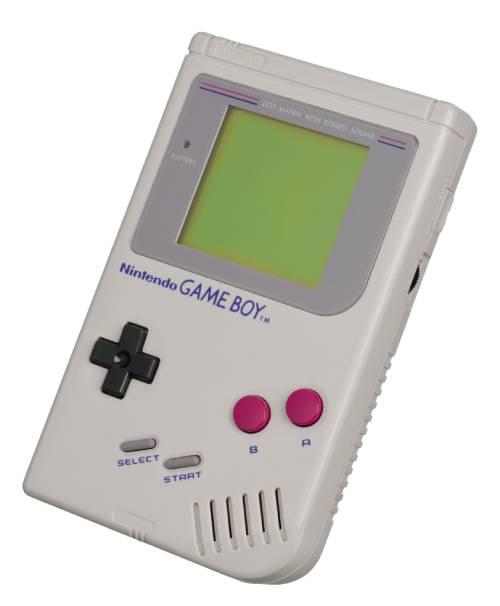
\includegraphics[width=0.15\textwidth]{include/images/gb.jpg}
\caption{Game Boy}
\label{figure:gb}
\end{figure}

Entre sus características técnicas, la Game Boy incluía un procesador Z80, una pantalla LCD monocromática con ajuste de contraste, un pad direccional de 8 direcciones, dos botones de acción (A y B) y dos botones de control (Start y Select).
\\\\
A pesar de recibir críticas por el tamaño de su pantalla y su limitada paleta de colores, la Game Boy logró un rotundo éxito comercial. Su éxito se atribuye principalmente a su bajo consumo energético, ya que funcionaba con cuatro pilas AA que ofrecían una gran autonomía en comparación con consolas rivales, como la Game Gear de SEGA. Además, la consola fue lanzada junto al exitoso juego Tetris, lo que contribuyó a su popularidad tanto entre niños como entre adultos.
\\\\
La longevidad de la Game Boy en el mercado se debe en gran parte al modelo de negocio que Nintendo continúa aplicando hoy en día, basado en la introducción de revisiones compatibles con versiones anteriores en lugar de lanzar consolas completamente nuevas. Entre estas revisiones destacan la Game Boy Pocket en 1996, así como la Game Boy Light y la Game Boy Color en 1998.

\begin{figure}[H]
\centering
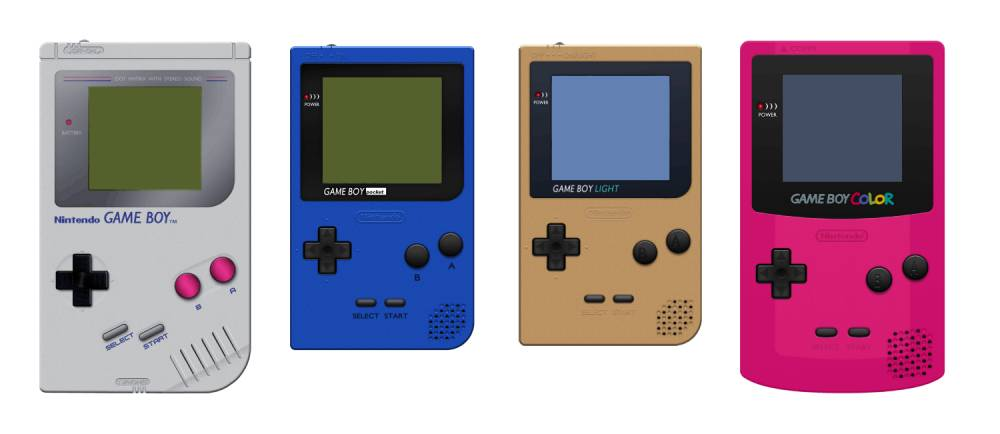
\includegraphics[width=0.7\textwidth]{include/images/gbs.jpg}
\caption{Versiones DMG, MGB, GBL y CGB de Game Boy}
\label{figure:v_gameboy}
\end{figure}

\subsection{Especificaciones Técnicas}

Cuando pensamos en programar un emulador que simule una máquina en concreto lo primero que debemos hacer es conocer exáctamente \textbf{cómo es por dentro y cómo funciona}. En la siguiente tabla quedan reflejadas todas las \textbf{características técnicas de la Game Boy}: \\

\begin{longtable}{|m{3cm}|m{2.5cm}|m{3cm}|m{2.5cm}|m{2.5cm}|}
\hline
\textbf{Características} & \textbf{Game Boy (DMG)} & \textbf{Game Boy Pocket (MGB)} & \textbf{Super Game Boy (SGB)} & \textbf{Game Boy Color (CGB)} \\
\hline
\endfirsthead
\multicolumn{5}{c}%
{\tablename\ \thetable\ -- \textit{Continúa de la página anterior}} \\
\hline
\textbf{Características} & \textbf{Game Boy (DMG)} & \textbf{Game Boy Pocket (MGB)} & \textbf{Super Game Boy (SGB)} & \textbf{Game Boy Color (CGB)} \\
\hline
\endhead
\hline \multicolumn{5}{|r|}{\textit{Continúa en la siguiente página}} \\
\endfoot
\hline
\endlastfoot

\textbf{CPU} & \multicolumn{4}{c|}{8-bit 8080-like Sharp CPU (speculated to be a SM83 core)}  \\
\hline
\textbf{Frecuencia CPU} & \multicolumn{2}{c|}{4.194304 MHz} & Depende de la revisión & Hasta 8.388608 MHz \\
\hline
\textbf{Work RAM} & \multicolumn{3}{c|}{8 KiB} & 32 KiB (4 + 7 × 4 KiB)  \\
\hline
\textbf{Video RAM} & \multicolumn{3}{c|}{8 KiB} & 16 KiB (2 × 8 KiB) \\
\hline
\textbf{Pantalla} & LCD 4.7 × 4.3 cm & LCD 4.8 × 4.4 cm & CRT TV & TFT 4.4 × 4 cm \\
\hline
\textbf{Resolución} & \multicolumn{2}{c|}{160 × 144} & 160 × 144 dentro de 256 × 224 border & 160 × 144 \\
\hline
\textbf{Sprites (OBJ)} & \multicolumn{4}{c|}{8×8 o 8×16; máximo 40 por pantalla, 10 por línea} \\
\hline
\textbf{Paletas} & \multicolumn{2}{c|}{BG: 1 × 4, OBJ: 2 × 3} & BG/OBJ: 1 + 4 × 3, border: 4 × 15 & BG: 8 × 4, OBJ: 8 × 33 \\
\hline
\textbf{Colores} & 4 tonos de verde & 4 tonos de gris & \multicolumn{2}{c|}{32768 colores (15-bit RGB)} \\
\hline
\textbf{Sincronización horizontal} & \multicolumn{2}{c|}{9.198 KHz} & Complicado\footnotemark[1] & 9.198 KHz \\
\hline
\textbf{Sincronización vertical} & \multicolumn{2}{c|}{59.73 Hz} & Complicado\footnotemark[1] & 59.73 Hz \\
\hline
\textbf{Sonido} & \multicolumn{2}{p{5cm}|}{4 canales con salida estéreo} & 4 canales GB + audio SNES & 4 canales con salida estéreo \\
\hline
\textbf{Energía} & DC 6V, 0.7 W & DC 3V, 0.7 W & Alimentado por SNES & DC 3V, 0.6 W \\
\hline

\caption{Especificaciones técnicas de la Game Boy.}
\label{table:1}
\end{longtable}

\footnotetext[1]{La SGB ejecuta dos consolas de forma simultánea: la Game Boy dentro del cartucho y la SNES. La SNES captura y muestra los gráficos de la Game Boy, pero las velocidades de fotogramas de ambas no se sincronizan completamente, lo que provoca duplicados y/o eliminados}

\subsection{Mapa de Memoria}

La Game Boy dispone de 64 Kb de memoria y utiliza direcciones de memoria de 16 bits, lo que le da la posibilidad de utilizar el rango de 0x0000 hasta 0xFFFF (65.535 bytes en total). Además, esta memoria se organiza en diferentes áreas para que el procesador pueda acceder a recursos clave como el código del juego, la memoria de video, la RAM y los registros de control. Cada una de estas áreas tiene una función específica, y algunas de ellas están sujetas a restricciones o condiciones de acceso durante la ejecución del sistema.

\begin{table}[h]
\centering
\begin{tabular}{|c|c|c|}
\hline
\textbf{Inicio} & \textbf{Fin} & \textbf{Descripción} \\ \hline
0000 & 3FFF & 16 KiB Banco ROM 00 \\ \hline
4000 & 7FFF & 16 KiB Banco ROM 01–NN \\ \hline
8000 & 9FFF & 8 KiB RAM de Vídeo (VRAM) \\ \hline
A000 & BFFF & 8 KiB RAM Externa \\ \hline
C000 & CFFF & 4 KiB Work RAM (WRAM) \\ \hline
D000 & DFFF & 4 KiB Work RAM (WRAM) \\ \hline
E000 & FDFF & Echo RAM (espejo de C000–DDFF) \\ \hline
FE00 & FE9F & Memoria de atributos de objetos (OAM) \\ \hline
FEA0 & FEFF & No usable \\ \hline
FF00 & FF7F & Registros de entrada/salida (I/O) \\ \hline
FF80 & FFFE & High RAM (HRAM) \\ \hline
FFFF & FFFF & Registro de habilitación de interrupciones (IE) \\ \hline
\end{tabular}
\caption{Mapa de memoria de Game Boy}
\end{table}

\subsubsection{ROM: [0x0000 - 0x7FFF]}
En las primeras direcciones del mapa de memoria (0x0000–0x7FFF) se encuentran los bancos de memoria ROM, que almacenan el código del juego cargado desde el cartucho. La sección entre 0x0000 y 0x3FFF es el banco fijo de 16 KiB que se carga automáticamente al encender la consola. Por último, la sección entre 0x4000 y 0x7FFF corresponde a bancos de ROM adicionales que pueden ser intercambiados (si el tipo de cartucho lo permite) para ofrecer acceso a más de 32 KiB de memoria.

\subsubsection{VRAM: [0x8000 - 0x9FFF]}
La VRAM es una memoria de 8 KiB que se utiliza para almacenar datos gráficos, como los sprites y tiles que se dibujan en pantalla. En los modelos CGB, esta sección de la memoria tiene dos bancos, con la posibilidad de intercambiarlos entre ellos y almacenar gráficos adicionales.

\subsubsection{RAM Externa: [0xA000 - 0xBFFF]}
Algunos cartuchos incluyen RAM adicional que se usa principalmente para guardar datos o estados del juego, como partidas guardadas. Esta RAM externa, que varía en tamaño según el cartucho, se puede acceder a través de esta región de memoria.

\subsubsection{Work RAM: [0xC000 - 0xDFFF]}
La WRAM es un área de memoria utilizada por el sistema para almacenar variables temporales, datos en proceso, y otra información necesaria para la ejecución de los programas. Está dividida en dos secciones de 4 KiB cada una. En los modelos CGB, la segunda parte (0xD000–0xDFFF) también puede ser conmutada entre diferentes bancos para aumentar la capacidad de almacenamiento.

\subsubsection{Echo RAM: [0xE000 - 0xFDFF]}
Esta es una copia exacta de la WRAM en las direcciones 0xC000–0xDDFF. Aunque se puede acceder a ella de la misma forma que la RAM original, Nintendo prohíbe su uso, ya que podría causar errores de sincronización o conflictos de acceso.

\subsubsection{OAM: [0xFE00 - 0xFE9F]}
La OAM es un pequeño bloque de memoria dedicado a almacenar información sobre los sprites que aparecen en pantalla, como su posición, prioridad y patrones de color. Puede contener hasta un total de 40 sprites, cada uno de 8x8 u 8x16 píxeles. Sin embargo, por limitaciones de hardware, solamente se pueden mostrar 10 sprites por scanline.

\subsubsection{No utilizable: [0xFEA0 - 0xFEFF]}
Esta pequeña área de memoria no se utiliza y está reservada. Cualquier intento de leer o escribir en esta región puede provocar comportamientos inesperados en el sistema.
\\\\
Si se intenta acceder a la región, devolverá un valor 0xFF cuando el OAM está bloqueado, y de lo contrario, dependerá de la revisión del hardware:

\begin{itemize}
    \item En DMG, MGB, SGB y SGB2, las lecturas durante el bloqueo de OAM provocan corrupción de OAM. De otra forma devolverán 0x00.
    \item En la revisión E de CGB, y los modelos AGB, AGS y GBP, devuelve el nibble alto del byte de la dirección inferior dos veces; por ejemplo, 0xFFA0 devuelve 0xAA, 0xFFB1 devuelve 0xBB, y así sucesivamente.
    \item En el resto de revisiones de CGB (0-D), la región es una sección de RAM única, pero enmascarada con un valor específico.
\end{itemize}

\subsubsection{I/O: [0xFEA0 - 0xFEFF]}
Estos registros se utilizan para controlar diferentes aspectos del hardware de la Game Boy, como la pantalla, los botones de entrada, el sonido y otros componentes del sistema. Acceder a estos registros permite al software interactuar directamente con el hardware.

\subsubsection{HRAM: [0xFF80 - 0xFFFE]}
La HRAM es un pequeño bloque de memoria de alta velocidad que contiene datos críticos que el procesador necesita acceder de manera rápida y frecuente.

\subsubsection{IE: 0xFFFF}
Registro de habilitación de interrupciones (Interrupt Enable), que permite activar o desactivar interrupciones específicas del sistema, cruciales para el manejo de eventos como temporizadores o actualizaciones gráficas.

\section{CPU}

También conocida como la Unidad Central de Procesamiento, que constituye el núcleo principal del sistema. Es la encargada de ejecutar los opcodes, que definen el comportamiento del software en la consola original.

\subsection{Diferencias}

LA Game Boy cuenta con un procesador único conocido como Sharp LR35902 y, como viene indicado en su nombre, fue desarrollado por la empresa Sharp Corporation. Esta CPU era una mezcla entre la conocida Zilog Z80 y el Intel 8080, a la cual se añadieron y eliminaron distintas instrucciones. Una diferencia importante, es que la Sharp no tiene instrucciones propias de I/O, a diferencia de las otras dos. En este caso, se puede acceder a los puertos de entrada/salida mediante comandos simples de carga (LD).
\\\\
A continuación se muestra una tabla con las diferencias existentes en el abanico de instrucciones:

\begin{table}[H]
    \centering
    \begin{tabular}{|c|c|c|}
        \hline
        \textbf{Opcode} & \textbf{Z80} & \textbf{Sharp LR35902} \\
        \hline
        08 & EX AF,AF & LD (nn),SP \\ \hline
        10 & DJNZ PC+dd & STOP \\ \hline
        22 & LD (nn),HL & LDI (HL),A \\ \hline
        2A & LD HL,(nn) & LDI A,(HL) \\ \hline
        32 & LD (nn),A & LDD (HL),A \\ \hline
        3A & LD A,(nn) & LDD A,(HL) \\ \hline
        D3 & OUT (n),A & - \\ \hline
        D9 & EXX & RETI \\ \hline
        DB & IN A,(n) & - \\ \hline
        DD & \textless IX\textgreater prefix & - \\ \hline
        E0 & RET PO & LD (FF00+n),A \\ \hline
        E2 & JP PO,nn & LD (FF00+C),A \\ \hline
        E3 & EX (SP),HL & - \\ \hline
        E4 & CALL P0,nn & - \\ \hline
        E8 & RET PE & ADD SP,dd \\ \hline
        EA & JP PE,nn & LD (nn),A \\ \hline
        EB & EX DE,HL & - \\ \hline
        EC & CALL PE,nn & - \\ \hline
        ED & \textless prefix\textgreater & - \\ \hline
        F0 & RET P & LD A,(FF00+n) \\ \hline
        F2 & JP P,nn & LD A,(FF00+C) \\ \hline
        F4 & CALL P,nn & - \\ \hline
        F8 & RET M & LD HL,SP+dd \\ \hline
        FA & JP M,nn & LD A,(nn) \\ \hline
        FC & CALL M,nn & - \\ \hline
        FD & \textless IY\textgreater prefix & - \\ \hline
        CB 3X & SLL r/(HL) & SWAP r/(HL) \\
        \hline
    \end{tabular}
    \caption{Comparación de opcodes entre Z80 y Sharp LR35902}
\end{table}

Los opcodes que se indican con un "-" significan que han sido eliminados. Si intentáramos utilizar los originales, la Game Boy simplemente se congelaría y habría que reiniciar el sistema.

\subsection{Registros}

Un registro es una pequeña unidad de almacenamiento en un procesador utilizada para guardar temporalmente datos o instrucciones durante la ejecución de operaciones. Los registros que se emplean son: A, F, B, C, D, E, H y L, cada uno capaz de almacenar 1 byte de información. Estos registros también pueden agruparse en pares para manejar 2 bytes: AF, BC, DE y HL. Adicionalmente, los registros SP (Stack Pointer) y PC (Program Counter) desempeñan funciones específicas dentro de la CPU.
\\\\
El primer registro a destacar es el registro A, conocido como el Acumulador, donde se almacena la mayoría de los datos procesados por la CPU. Es un registro al que se le pueden asignar valores de forma directa, al igual que ocurre con los registros B, C, D, E, H y L.
\\\\
Los registros B y C son comúnmente utilizados como contadores, mientras que los registros D y E se suelen emplear en pares para almacenar direcciones de memoria, facilitando operaciones de copia de datos. Sin embargo, el uso de estos registros no está limitado a estos propósitos; su aplicación depende de las necesidades y la conveniencia del programador.
\\\\
El registro F o Flags es responsable de almacenar el estado actual del procesador, y es de solo lectura. Aunque no se puede modificar directamente, su combinación con el registro A es clave para realizar diversas operaciones. Su principal utilidad radica en la evaluación de los resultados de la instrucción anterior, siendo esencial para la toma de decisiones en la ejecución del programa.
\\\\
En la siguiente tabla podemos ver el desglose del valor atribuido a cada bit del registro F:

\begin{table}[H]
    \centering
    \begin{tabular}{|c|c|>{\centering\arraybackslash}p{9cm}|}
        \hline
        \textbf{Bit} & \textbf{Nombre} & \textbf{Definición} \\
        \hline
        7 & Z & Zero: indica si el resultado de la operación previa ha dado como resultado 0. \\
        \hline
        6 & N & Substraction: indica si la operación previa ha sido una resta. \\
        \hline
        5 & H & Semi-Carry: indica si se ha producido un acarreo desde el nibble bajo al alto en la operación de suma o resta anterior. \\
        \hline
        4 & C o CY & Carry: indica si se ha producido un acarreo en el bit más significativo, es decir, el resultado ha sido mayor de 0xFF. \\
        \hline
        3-0 & - & No se utilizan. \\
        \hline
    \end{tabular}
    \caption{Función de los bits del registro F o Flags}
\end{table}

Por su parte, los registros H y L se utilizan para el acceso indirecto a una dirección de memoria. Este acceso indirecto se refiere al valor de 16 bits contenido en la pareja de registros HL, y resulta especialmente útil para recorrer arrays o acceder secuencialmente a posiciones de memoria.
\\\\
El registro SP (Stack Pointer) señala la posición de memoria que se utiliza durante las llamadas a subrutinas. Al ejecutar una instrucción call, la pila aumenta, y al realizar un ret, la pila disminuye, permitiendo mantener el control del flujo de ejecución.
\\\\
Finalmente, el registro PC (Program Counter) indica la dirección de memoria donde se encuentra la próxima instrucción que será ejecutada por la CPU, siendo esencial para el flujo de control del programa.

\subsection{Opcodes}

Los opcodes (códigos de operación) son las instrucciones que un procesador entiende y ejecuta directamente. Representan la parte de una instrucción de máquina que especifica la operación a realizar, como cargar datos en un registro, realizar una operación matemática o mover datos entre la memoria y el procesador. Cada opcode tiene un formato específico y puede estar compuesto por varios bytes que definen tanto la operación como los operandos involucrados.

\subsubsection{Categorías}

En total, existen 510 instrucciones diferentes, las cuales pueden ser agrupadas en las siguientes categorías:
\begin{itemize}
  \item \textbf{Operaciones de carga (LD)}
  \begin{itemize}
  \item LD A, (HL): Carga el valor de la dirección de memoria en el registro A.
  \item LD (HL), B: Carga el valor del registro B en la memoria apuntada por HL.
  \end{itemize}
  \item \textbf{Operaciones aritméticas y lógicas}
  \begin{itemize}
  \item ADD A, B: Suma el contenido de B al registro A.
  \item AND A: Realiza una operación lógica AND en el registro A.
  \item SUB A, B: Resta el valor de B del registro A.
  \item XOR A: Realiza una operación XOR entre el registro A consigo mismo, lo que siempre da como resultado 0. Este comando se utiliza para limpiar o reiniciar el registro A.
  \item OR A: Realiza una operación OR del registro A consigo mismo, dejando el valor de A sin cambios. No afecta el valor, pero puede modificar los flags.
  \item CP A: Compara el valor del registro A con el valor de otro registro o inmediato, estableciendo los flags según el resultado de la comparación. La operación es similar a una resta (A - valor) y no modifica el contenido de A.
  \item CPL: Complementa el valor del registro A, invirtiendo todos sus bits. Esta operación afecta el flag de medio acarreo (H) y establece el flag de negativo (N).
  \item CCF: Cambia el estado del flag de acarreo (C). Si el flag de acarreo está establecido, se limpia; si está limpio, se establece. Esta operación no afecta a los demás flags.
  \item DAA: Ajusta el contenido del registro A para que represente un valor decimal válido, teniendo en cuenta el estado de los flags de acarreo (C) y medio acarreo (H). Esta operación es útil después de realizar operaciones aritméticas en el modo BCD.
  \item SCF: Establece el flag de acarreo (C) y limpia el flag de acarreo (H). Esta operación no afecta a los demás flags y es útil para preparar operaciones que requieren un estado de acarreo conocido.
  \end{itemize}
  \item \textbf{Operaciones de control de flujo}
  \begin{itemize}
  \item JP nn: Salta a la dirección de memoria nn.
  \item CALL nn: Llama a una subrutina en la dirección nn.
  \item RET: Retorna de una subrutina.
  \end{itemize}
  \item \textbf{Operaciones de rotación y desplazamiento}
  \begin{itemize}
  \item RL A: Rota los bits del registro A hacia la izquierda a través del carry.
  \item SLA B: Desplaza los bits de B hacia la izquierda.
  \item RR A: Rota los bits del registro A hacia la derecha a través del carry, trasladando el bit menos significativo al carry y el carry al bit más significativo.
  \item RLC A: Rota los bits del registro A hacia la izquierda, desplazando el bit más significativo al carry y reiniciando el bit más significativo con el valor original del carry.
  \item RRC A: Rota los bits del registro A hacia la derecha, moviendo el bit menos significativo al carry y llenando el bit más significativo con el valor del carry.
  \item SRA B: Desplaza los bits de B hacia la derecha, manteniendo el bit más significativo (signo) constante y colocando el bit menos significativo en el carry.
  \item SWAP B: Intercambia los cuatro bits más significativos con los cuatro menos significativos del registro B.
  \item SRL B: Desplaza los bits de B hacia la derecha, moviendo el bit menos significativo al carry y rellenando el bit más significativo con 0.
  \end{itemize}
  \item \textbf{Operaciones de manipulación de bits}
  \begin{itemize}
  \item BIT 0, A: Prueba si el bit 0 de A está establecido.
  \item SET 1, (HL): Establece el bit 1 en la dirección de memoria HL.
  \item RES 0, A: Reinicia (pone a 0) el LSB del registro A, dejando los demás bits sin cambios.
  \end{itemize}
  \item \textbf{Operaciones especiales de sistema}
  \begin{itemize}
  \item NOP: No realiza ninguna operación.
  \item DI: Deshabilita interrupciones.
  \item EI: Habilita interrupciones.
  \end{itemize}
  \item \textbf{Operaciones con pila}
  \begin{itemize}
  \item PUSH BC: Empuja el contenido del registro BC en la pila.
  \item POP AF: Restaura el contenido de AF desde la pila.
  \end{itemize}
  \item \textbf{Operaciones I/O}
  \begin{itemize}
  \item LD (FF00+n), A: Carga el valor de A en la dirección de I/O FF00+n.
  \item LD A, (FF00+C): Carga el valor de la dirección FF00+C en A.
  \end{itemize}
\end{itemize}

\subsubsection{Listado}
Para poder empezar a implementar todos los opcodes, debemos hacer uso de la documentación (oficial o no) que nos indique qué Byte hace referencia a qué opcode. Las siguientes tablas suelen ser de gran ayuda para verlo de forma clara y concisa:

\begin{figure}[H]
\centering
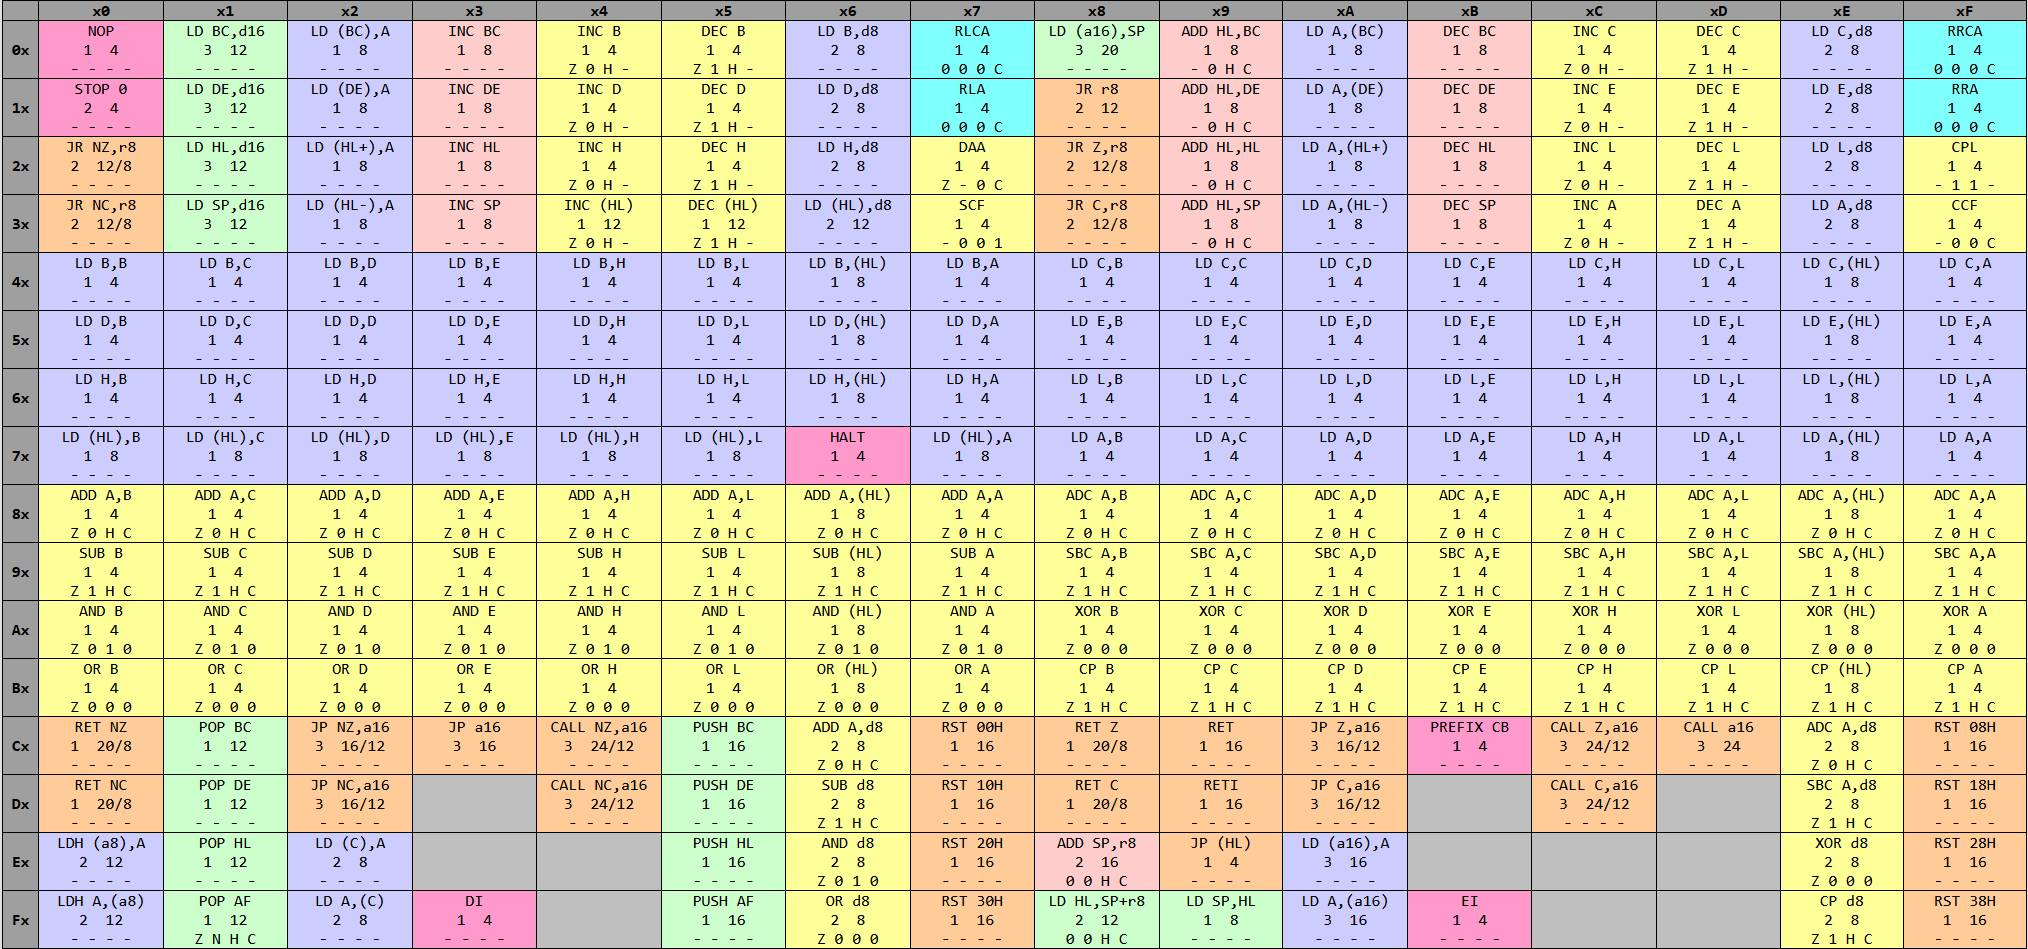
\includegraphics[width=1\textwidth]{include/images/opcodes_1.jpg}
\caption{Set de Instrucciones}
\label{figure:opcodes_1}
\end{figure}

\begin{figure}[H]
\centering
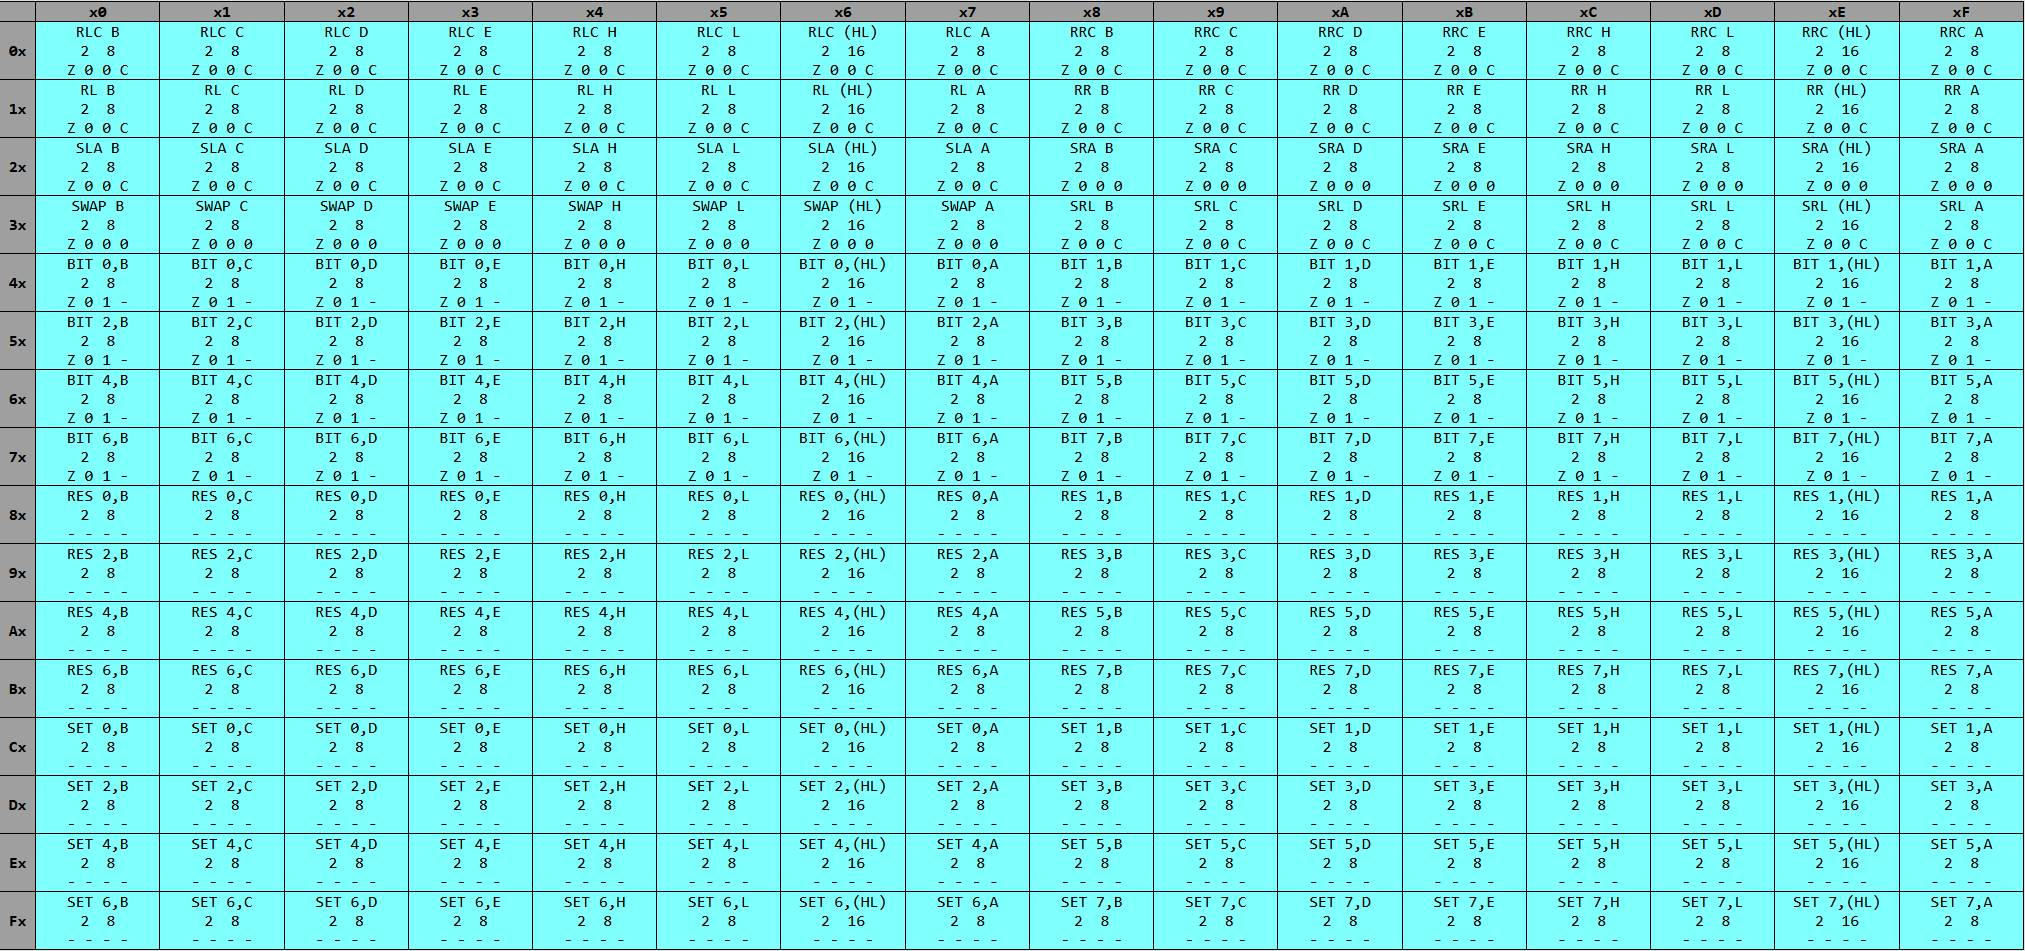
\includegraphics[width=1\textwidth]{include/images/opcodes_2.jpg}
\caption{Set de Instrucciones Extendidas}
\label{figure:opcodes_2}
\end{figure}

Con estas tablas obtenemos las siguientes características de cada instrucción:
\begin{itemize}
    \item \textbf{Byte} asignado.
    \item \textbf{Ciclos} de reloj.
    \item \textbf{Flags} a ignorar, actualizar o resetear.
    \item \textbf{Categoría}, agrupados por colores.
    \item \textbf{Longitud}, es decir, los bytes que la instrucción va a ocupar en memoria.
\end{itemize}

\subsection{Ciclos}

Los ciclos de CPU son unidades de tiempo en las que se realizan instrucciones. Son utilizadas para saber con exactitud cuánto tiempo dura la ejecución de una instrucción concreta en el hardware original. Hay dos conceptos distintos en este contexto: ciclos de máquina y ciclos de reloj.
\\\\
Cada componente, como la CPU, la memoria, el PPU y el APU, opera en función de los ciclos de reloj. La coordinación precisa entre estos módulos asegura que las instrucciones se ejecuten en el momento adecuado y que los datos se transfieran de manera eficiente.
\\\\
Por ejemplo, el procesador necesita esperar que el PPU complete la renderización de un cuadro antes de actualizar la pantalla, lo que implica un control cuidadoso del tiempo. Si un módulo se desincroniza, puede resultar en fallos gráficos, sonido entrecortado o un rendimiento general deficiente. Por lo tanto, la medición de ciclos de reloj permite establecer un ritmo de operación coherente, asegurando que todos los componentes funcionen armónicamente, lo que es fundamental para la experiencia de juego fluida y efectiva que caracteriza a la Game Boy.
\\\\
Para la Game Boy, 1 ciclo de máquina equivale a 4 ciclos de reloj.

\subsubsection{Ciclos de Máquina}
Los ciclos de máquina se refieren a la cantidad de ciclos de CPU necesarios para ejecutar una instrucción específica. Cada instrucción puede requerir un número diferente de ciclos de máquina, dependiendo de su complejidad.

\subsubsection{Ciclos de Reloj}
Los ciclos de reloj, por otro lado, son las unidades de tiempo que marcan el ritmo del funcionamiento del procesador. Cada ciclo de reloj representa un pulso generado por un oscilador interno en el procesador, que sincroniza las operaciones del mismo. La frecuencia del reloj, medida en hertzios (Hz), determina cuántos ciclos de reloj se producen por segundo.

\section{ROM}
\subsection{Secuencia de Arranque}

Existe una secuencia de arranque, conocido como \textbf{Boot ROM}, guardado dentro de la propia CPU. Esta secuencia de arranque comienza su ejecución en la dirección de memoria 0x000, y no en la oficial de 0x100. Este programa es responsable de la animación de arranque que se reproduce antes de que el control sea transferido a la ROM del cartucho, además de inicializar distintos registros y direcciones de memoria.
\\\\
Existen en total 9 programas de boot (conocidos hasta la fecha):
\begin{table}[h!]
\centering
\begin{tabular}{|l|c|}
\hline
\textbf{Nombre} & \textbf{Tamaño (bytes)} \\ \hline
DMG0 & 256 \\ \hline
DMG  & 256 \\ \hline
MGB  & 256 \\ \hline
SGB  & 256 \\ \hline
SGB2 & 256 \\ \hline
CGB0 & 256 + 1792 \\ \hline
CGB  & 256 + 1792 \\ \hline
AGB0 & 256 + 1792 \\ \hline
AGB  & 256 + 1792 \\ \hline
\end{tabular}
\caption{Resumen de las variaciones de las secuencias de arranque}
\end{table}

\subsubsection{DMG / MGB}
Lo primero que hacen es leer el logo desde el cartucho, descomprimirlo en VRAM y comenzar a desplazarlo lentamente hacia abajo. Dado que las lecturas de un cartucho ausente generalmente devuelven 0xFF, esto explica por qué, al encender la consola sin un cartucho, aparece un cuadro negro desplazándose. Además, conexiones defectuosas o sucias pueden hacer que los datos leídos se corrompan, lo que resulta en un logo desordenado.
\\\\
Una vez que el logo ha terminado de desplazarse, la boot ROM reproduce el famoso sonido \textit{"ba-ding!”} y vuelve a leer el logo, esta vez comparándolo con una copia almacenada en ROM. También calcula el checksum del encabezado y lo compara con el checksum almacenado en el encabezado. Si alguna de estas verificaciones falla, la boot ROM se bloquea y nunca se transfiere el control a la ROM del cartucho.
\\\\
Finalmente, la boot ROM escribe en el registro BANK en 0xFF50, lo que desasigna la boot ROM.
\\\\
Las diferencias con DMG0 (algunos primeros modelos de DMG), es que al fallar el checksum, la pantalla empieza a parpadear a la hora de bloquear la ROM, y que el logo de Nintendo no tiene el símbolo ®.

\subsubsection{CGB / AGB}
Estas secuencias de arranque son mucho más complejas, en especial por su comportamiento de retro-compatibilidad.
\\\\
La ROM de arranque es más grande. Aún debe ser mapeada comenzando en 0x0000, ya que es donde comienza la CPU, pero también debe acceder al encabezado del cartucho en 0x0100-0x014F. Por lo tanto, la ROM de arranque se divide en dos partes: una de 0x0000-0x00FF y otra de 0x0200-0x08FF.
\\\\
Primero, las ROMs de arranque descomponen el logo de Nintendo en VRAM, al igual que los modelos antiguos, y copian el logo a un búfer en HRAM al mismo tiempo.
\\\\
Luego, el logo se lee y descomprime nuevamente, pero sin redimensionamiento, lo que produce un logo mucho más pequeño colocado debajo del gran \textit{"GAME BOY"}. La ROM de arranque luego configura las paletas de compatibilidad, como se describe más adelante, y reproduce la animación del logo con el sonido de \textit{"ba-ding!"}.
\\\\
Durante la animación del logo, se permite al usuario elegir una paleta para anular la seleccionada para compatibilidad (con distintas secuencias de botones). Cada nueva elección evita que la animación termine durante 30 fotogramas, lo que retrasa el checksum y la transición final.
\\\\
Finalmente, la ROM de arranque desvanece todas las paletas de Background a blanco y establece el hardware en modo de compatibilidad (recordemos que existen juegos como Pokémon Oro/Plata que son de GBC pero se pueden jugar en DMG). En función del valor del byte de compatibilidad CGB, los valores a insertar en distintos registros de CGB variarán.

\subsection{Cabecera del Cartucho}

Todos los cartuchos de Game Boy contienen una cabecera ubicada en el rango de direcciones 0x100-0x14F. Esta cabecera contiene información esencial para el funcionamiento del juego y del sistema, permitiendo a los desarrolladores configurar diversos parámetros que describen las características del cartucho. Entre estos parámetros se incluyen el título del juego, el código de licencia, el tipo de cartucho (que define si utiliza RAM, batería, o expansión como MBC), y otros datos relevantes. A continuación, se detallan los registros presentes en este rango de direcciones:

\subsubsection{0x0100 - 0x0103: Punto de entrada}
Después de mostrar el logotipo de Nintendo, el PC salta a la dirección 0x0100, para a posterior saltar al inicio del programa del juego. La mayoría de los desarrolladores llenan esta área de 4 bytes con una instrucción NOP seguida de un JP 0x0150.

\subsubsection{0x0104 - 0x0133: Nintendo logo}
Esta área contiene una imagen en mapa de bits que se muestra cuando se enciende la consola. Debe coincidir con el siguiente volcado (en hexadecimal); de lo contrario, la ROM de arranque no permitirá que el juego se ejecute:

\begin{lstlisting}[language=Kotlin, caption={Nintendo Logo - Mapa de Bits}, label={code:nintendologobits}]
    CE ED 66 66 CC 0D 00 0B 03 73 00 83 00 0C 00 0D
    00 08 11 1F 88 89 00 0E DC CC 6E E6 DD DD D9 99
    BB BB 67 63 6E 0E EC CC DD DC 99 9F BB B9 33 3E
\end{lstlisting}

La forma en la que estos bytes se decodifican es la siguiente:
\begin{itemize}
    \item Los bytes en el rango 0x104-0x011B representan la mitad superior del logo, mientras que los del rango 0x11C-0x133 representan la mitad inferior.
    \item Por cada byte, cada nibble codifica 4 píxeles. Un pixel está encendido si su bit correspondiente tiene un valor de 1.
    \item Cada dos bytes componen un grupo, el cual representa una parte (inferior o superior) de una letra del logo.
\end{itemize}

\begin{figure}[H]
\centering
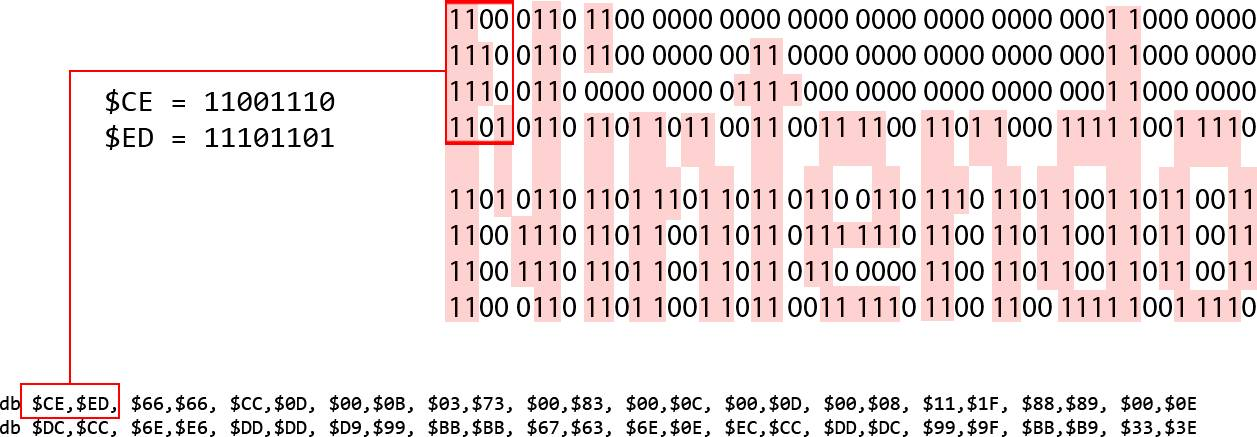
\includegraphics[width=1\textwidth]{include/images/dibujado_logo_n.jpg}
\caption{Decodificación del logo de Nintendo}
\label{figure:decodednlogo}
\end{figure}

El procedimiento de arranque de la Game Boy primero muestra el logo y luego verifica que coincida con el volcado anterior (conocido como \textit{checksum}). Si no coincide, la ROM de arranque se bloquea.
\\\\
Los modelos a partir del CGB solo verifican la mitad superior (los primeros 18 bytes).

\subsubsection{0x0134 - 0x0143: Título}
Esta región de bytes contienen el título del juego, con carácteres ASCII y completamente en mayúsculas. Si el título tiene menos de 16 carácteres, el resto de bytes deberán rellenarse con 0x00's. 
\\\\
En versiones posteriores de los cartuchos, partes de esta área tienen un significado diferente, lo que reduce el tamaño real a 15 u 11 carácteres (siempre empezando en la dirección 0x134).

\subsubsection{0x013F - 0x0142: Código de fabricante}

En los cartuchos más antiguos, estos bytes formaban parte del título. En los cartuchos más nuevos, contienen un código de fabricante de 4 caracteres (en mayúsculas ASCII). Se desconoce su propósito.

\subsubsection{0x0143: CGB Flag}
Este byte, al igual que con el código de fabricante, formaba parte del título. Los modelos CGB y posteriores lo interpretan para decidir si habilitan el modo Color ("Modo CGB") o si retroceden al modo de compatibilidad monocromático ("Modo no CGB").
\\\\
Los valores más típicos son: 
\begin{itemize}
    \item 0x00: No indicaría nada realmente, lo que implica que el juego solamente funciona en modelos DMG/MGB.
    \item 0x80: Indica que el juego admite mejoras propias del modelo CGB, pero es retro-compatible con modelos anteriores (DMG, MGB, etc...).
    \item 0xC0: El juego solamente funciona en CGB.
\end{itemize}

Valores que tengan activados los bits 7, 3 o 2, activarán un estado poco utilizado, conocido como "Modo PGB" (Pseudo Game Boy Mode). Es una especie de modo intermedio que brinda compatibilidad con juegos diseñados para el Game Boy Color cuando se ejecutan en un Game Boy original o en un Super Game Boy, pero con mejoras visuales muy limitadas en comparación con el modo CGB completo.
\\\\
Hay poca información al respecto de este modo y varias fuentes agradecen su estudio y documentación.

\subsubsection{0x0144 – 0x0145: Nuevo código de licencia}
Esta región contiene un código representado por dos carácteres ASCII, el cual indica el editor/desarrollador del juego. Solamente se utiliza en caso de que el antiguo código de licencia tenga un valor de 0x33 (suele ser el caso para los juegos publicados después de la salida de SGB).
\\\\
Los códigos son los siguientes:
\begin{longtable}{|c|l|}
\hline
\textbf{Código} & \textbf{Editor} \\ \hline
00              & Ninguno                        \\ \hline
01              & Nintendo Research \& Development 1 \\ \hline
08              & Capcom                         \\ \hline
13              & EA (Electronic Arts)           \\ \hline
18              & Hudson Soft                    \\ \hline
19              & B-AI                           \\ \hline
20              & KSS                            \\ \hline
22              & Oficina de Planificación WADA  \\ \hline
24              & PCM Complete                   \\ \hline
25              & San-X                          \\ \hline
28              & Kemco                          \\ \hline
29              & SETA Corporation               \\ \hline
30              & Viacom                         \\ \hline
31              & Nintendo                       \\ \hline
32              & Bandai                         \\ \hline
33              & Ocean Software/Acclaim Entertainment \\ \hline
34              & Konami                         \\ \hline
35              & HectorSoft                     \\ \hline
37              & Taito                          \\ \hline
38              & Hudson Soft                    \\ \hline
39              & Banpresto                      \\ \hline
41              & Ubi Soft                       \\ \hline
42              & Atlus                          \\ \hline
44              & Malibu Interactive             \\ \hline
46              & Angel                          \\ \hline
47              & Bullet-Proof Software          \\ \hline
49              & Irem                           \\ \hline
50              & Absolute                       \\ \hline
51              & Acclaim Entertainment          \\ \hline
52              & Activision                     \\ \hline
53              & Sammy USA Corporation          \\ \hline
54              & Konami                         \\ \hline
55              & Hi Tech Expressions            \\ \hline
56              & LJN                            \\ \hline
57              & Matchbox                       \\ \hline
58              & Mattel                         \\ \hline
59              & Milton Bradley Company         \\ \hline
60              & Titus Interactive              \\ \hline
61              & Virgin Games Ltd.              \\ \hline
64              & Lucasfilm Games                \\ \hline
67              & Ocean Software                 \\ \hline
69              & EA (Electronic Arts)           \\ \hline
70              & Infogrames                     \\ \hline
71              & Interplay Entertainment        \\ \hline
72              & Broderbund                     \\ \hline
73              & Sculptured Software            \\ \hline
75              & The Sales Curve Limited        \\ \hline
78              & THQ                            \\ \hline
79              & Accolade                       \\ \hline
80              & Misawa Entertainment           \\ \hline
83              & lozc                           \\ \hline
86              & Tokuma Shoten                  \\ \hline
87              & Tsukuda Original               \\ \hline
91              & Chunsoft Co.                   \\ \hline
92              & Video System                   \\ \hline
93              & Ocean Software/Acclaim Entertainment \\ \hline
95              & Varie                          \\ \hline
96              & Yonezawa/s’pal                 \\ \hline
97              & Kaneko                         \\ \hline
99              & Pack-In-Video                  \\ \hline
9H              & Bottom Up                      \\ \hline
A4              & Konami (Yu-Gi-Oh!)             \\ \hline
BL              & MTO                            \\ \hline
DK              & Kodansha                       \\ \hline
\caption{Código de licencia y su editor.} \\
\end{longtable}

\subsubsection{0x0146: SGB Flag}
Especifica si el juego es compatible con funciones del modelo SGB. El SGB ignorará cualquier transferencia de datos si el valor de este byte no es 0x03.

\subsubsection{0x0147: Tipo de cartucho}
Especifica qué tipo de hardware está presente en el cartucho (para ser más especifico, su \textit{mapper}).
\\\\
Los mappers son los siguientes:
\begin{longtable}{|c|l|}
\hline
\textbf{Código} & \textbf{Tipo} \\
\hline
0x00 & ROM ONLY \\ \hline
0x01 & MBC1 \\ \hline
0x02 & MBC1+RAM \\ \hline
0x03 & MBC1+RAM+BATTERY \\ \hline
0x05 & MBC2 \\ \hline
0x06 & MBC2+BATTERY \\ \hline
0x08 & ROM+RAM \\ \hline
0x09 & ROM+RAM+BATTERY \\ \hline
0x0B & MMM01 \\ \hline
0x0C & MMM01+RAM \\ \hline
0x0D & MMM01+RAM+BATTERY \\ \hline
0x0F & MBC3+TIMER+BATTERY \\ \hline
0x10 & MBC3+TIMER+RAM+BATTERY \\ \hline
0x11 & MBC3 \\ \hline
0x12 & MBC3+RAM \\ \hline
0x13 & MBC3+RAM+BATTERY \\ \hline
0x19 & MBC5 \\ \hline
0x1A & MBC5+RAM \\ \hline
0x1B & MBC5+RAM+BATTERY \\ \hline
0x1C & MBC5+RUMBLE \\ \hline
0x1D & MBC5+RUMBLE+RAM \\ \hline
0x1E & MBC5+RUMBLE+RAM+BATTERY \\ \hline
0x20 & MBC6 \\ \hline
0x22 & MBC7+SENSOR+RUMBLE+RAM+BATTERY \\ \hline
0xFC & POCKET CAMERA \\ \hline
0xFD & BANDAI TAMA5 \\ \hline
0xFE & HuC3 \\ \hline
0xFF & HuC1+RAM+BATTERY \\ \hline
\caption{Tipos de mapeadores (MBC) y sus códigos} \\
\end{longtable}

\subsubsection{0x0148: Tamaño de ROM}
Indica el tamaño de ROM en el cartucho. En la mayoría de casos, se calcula como $32 KiB * (1 << valor)$. Los valores conocidos son:

\begin{table}[h]
    \centering
    \begin{tabular}{|c|c|c|}
        \hline
        \textbf{Valor} & \textbf{Tamaño} & \textbf{Número de bancos} \\
        \hline
        0x00 & 32 KiB & 2 \\ \hline
        0x01 & 64 KiB & 4 \\ \hline
        0x02 & 128 KiB & 8 \\ \hline
        0x03 & 256 KiB & 16 \\ \hline
        0x04 & 512 KiB & 32 \\ \hline
        0x05 & 1 MiB & 64 \\ \hline
        0x06 & 2 MiB & 128 \\ \hline
        0x07 & 4 MiB & 256 \\ \hline
        0x08 & 8 MiB & 512 \\ \hline
    \end{tabular}
    \caption{Tamaño y número de bancos de ROM según el valor especificado.}
    \label{tab:rom_size_banks}
\end{table}

\subsubsection{0x0149: Tamaño de RAM}
Indica el tamaño de RAM (si lo hay). Si el tipo de cartucho no incluye "RAM" en su nombre, el valor de este registro debe ser 0x00. 
\\\\
Los posibles tamaños son los siguientes:

\begin{table}[H]
    \centering
    \begin{tabular}{|c|c|l|}
        \hline
        \textbf{Código} & \textbf{Tamaño de SRAM} & \textbf{Comentario} \\ \hline
        0x00 & 0 & Sin RAM \\ \hline
        0x01 & – & No utilizado \\ \hline
        0x02 & 8 KiB & 1 banco \\ \hline
        0x03 & 32 KiB & 4 bancos de 8 KiB cada uno \\ \hline
        0x04 & 128 KiB & 16 bancos de 8 KiB cada uno \\ \hline
        0x05 & 64 KiB & 8 bancos de 8 KiB cada uno \\ \hline
    \end{tabular}
    \caption{Tamaño de SRAM según el código del cartucho.}
    \label{tab:sram_size}
\end{table}

El valor 0x01 aparece en algunos documentos no oficiales con un tamaño de 2KiB. Sin embargo, jamás se llegó a utilizar un chip de RAM con este tamaño. Algunas ROMs de dominio público utilizan este valor, aunque en su código no hacen uso de ningún tipo de RAM de cartucho.

\subsubsection{0x014A: Destino}
Especifica si el juego está destinado a ser vendido en Japón o en cualquier otro lugar del mundo. Existen dos posibles valores:

\begin{itemize}
    \item 0x00: Japón. Se puede vender en el extranjero.
    \item 0x01: Solamente en el extranjero.
\end{itemize}

\subsubsection{0x014B: Antiguo código de licencia}
Utilizado en cartuchos anteriores al lanzamiento del SGB. Al igual que el nuevo (0x0144-0x0145), especifica el editor/publisher. Si el valor es 0x33, se deberán utilizar los nuevos códigos.
\\\\
A continuación la lista de códigos y sus editores:
\begin{longtable}{|c|l|}
\hline
\textbf{Código} & \textbf{Editor} \\ \hline
00 & Ninguno \\\hline
01 & Nintendo \\\hline
08 & Capcom \\\hline
09 & HOT-B \\\hline
0A & Jaleco \\\hline
0B & Coconuts Japan \\\hline
0C & Elite Systems \\\hline
13 & EA (Electronic Arts) \\\hline
18 & Hudson Soft \\\hline
19 & ITC Entertainment \\\hline
1A & Yanoman \\\hline
1D & Japan Clary \\\hline
1F & Virgin Games Ltd.3 \\\hline
24 & PCM Complete \\\hline
25 & San-X \\\hline
28 & Kemco \\\hline
29 & SETA Corporation \\\hline
30 & Infogrames5 \\\hline
31 & Nintendo \\\hline
32 & Bandai \\\hline
33 & Se debe usar el nuevo código de licencia. \\\hline
34 & Konami \\\hline
35 & HectorSoft \\\hline
38 & Capcom \\\hline
39 & Banpresto \\\hline
3C & Entertainment Interactive (stub) \\\hline
3E & Gremlin \\\hline
41 & Ubi Soft1 \\\hline
42 & Atlus \\\hline
44 & Malibu Interactive \\\hline
46 & Angel \\\hline
47 & Spectrum HoloByte \\\hline
49 & Irem \\\hline
4A & Virgin Games Ltd.3 \\\hline
4D & Malibu Interactive \\\hline
4F & U.S. Gold \\\hline
50 & Absolute \\\hline
51 & Acclaim Entertainment \\\hline
52 & Activision \\\hline
53 & Sammy USA Corporation \\\hline
54 & GameTek \\\hline
55 & Park Place13 \\\hline
56 & LJN \\\hline
57 & Matchbox \\\hline
59 & Milton Bradley Company \\\hline
5A & Mindscape \\\hline
5B & Romstar \\\hline
5C & Naxat Soft14 \\\hline
5D & Tradewest \\\hline
60 & Titus Interactive \\\hline
61 & Virgin Games Ltd.3 \\\hline
67 & Ocean Software \\\hline
69 & EA (Electronic Arts) \\\hline
6E & Elite Systems \\\hline
6F & Electro Brain \\\hline
70 & Infogrames5 \\\hline
71 & Interplay Entertainment \\\hline
72 & Broderbund \\\hline
73 & Sculptured Software6 \\\hline
75 & The Sales Curve Limited7 \\\hline
78 & THQ \\\hline
79 & Accolade15 \\\hline
7A & Triffix Entertainment \\\hline
7C & MicroProse \\\hline
7F & Kemco \\\hline
80 & Misawa Entertainment \\\hline
83 & LOZC G. \\\hline
86 & Tokuma Shoten \\\hline
8B & Bullet-Proof Software2 \\\hline
8C & Vic Tokai Corp.16 \\\hline
8E & Ape Inc.17 \\\hline
8F & I’Max18 \\\hline
91 & Chunsoft Co.8 \\\hline
92 & Video System \\\hline
93 & Tsubaraya Productions \\\hline
95 & Varie \\\hline
96 & Yonezawa19/S’Pal \\\hline
97 & Kemco \\\hline
99 & Arc \\\hline
9A & Nihon Bussan \\\hline
9B & Tecmo \\\hline
9C & Imagineer \\\hline
9D & Banpresto \\\hline
9F & Nova \\\hline
A1 & Hori Electric \\\hline
A2 & Bandai \\\hline
A4 & Konami \\\hline
A6 & Kawada \\\hline
A7 & Takara \\\hline
A9 & Technos Japan \\\hline
AA & Broderbund \\\hline
AC & Toei Animation \\\hline
AD & Toho \\\hline
AF & Namco \\\hline
B0 & Acclaim Entertainment \\\hline
B1 & ASCII Corporation or Nexsoft \\\hline
B2 & Bandai \\\hline
B4 & Square Enix \\\hline
B6 & HAL Laboratory \\\hline
B7 & SNK \\\hline
B9 & Pony Canyon \\\hline
BA & Culture Brain \\\hline
BB & Sunsoft \\\hline
BD & Sony Imagesoft \\\hline
BF & Sammy Corporation \\\hline
C0 & Taito \\\hline
C2 & Kemco \\\hline
C3 & Square \\\hline
C4 & Tokuma Shoten \\\hline
C5 & Data East \\\hline
C6 & Tonkin House \\\hline
C8 & Koei \\\hline
C9 & UFL \\\hline
CA & Ultra Games \\\hline
CB & VAP, Inc. \\\hline
CC & Use Corporation \\\hline
CD & Meldac \\\hline
CE & Pony Canyon \\\hline
CF & Angel \\\hline
D0 & Taito \\\hline
D1 & SOFEL (Software Engineering Lab) \\\hline
D2 & Quest \\\hline
D3 & Sigma Enterprises \\\hline
D4 & ASK Kodansha Co. \\\hline
D6 & Naxat Soft14 \\\hline
D7 & Copya System \\\hline
D9 & Banpresto \\\hline
DA & Tomy \\\hline
DB & LJN \\\hline
DD & Nippon Computer Systems \\\hline
DE & Human Ent. \\\hline
DF & Altron \\\hline
E0 & Jaleco \\\hline
E1 & Towa Chiki \\\hline
E2 & Yutaka \\\hline
E3 & Varie \\\hline
E5 & Epoch \\\hline
E7 & Athena \\\hline
E8 & Asmik Ace Entertainment \\\hline
E9 & Natsume \\\hline
EA & King Records \\\hline
EB & Atlus \\\hline
EC & Epic/Sony Records \\\hline
EE & IGS \\\hline
F0 & A Wave \\\hline
F3 & Extreme Entertainment \\\hline
FF & LJN \\\hline
\caption{Antiguos códigos de licencia y su editor.}
\end{longtable}

\subsubsection{0x014C: Número de versión de ROM}
Este byte especifica el número de versión del juego. Generalmente es 0x00. Puede ser útil para los desarrolladores y emuladores, por ejemplo, para aplicar parches o actualizaciones específicas que se hayan diseñado para esa versión (importante en juegos que recibieron revisiones).

\subsubsection{0x014D: Checksum}
Este byte contiene una suma de verificación de 8 bits calculada a partir de los bytes de cabecera del cartucho 0x0134–0x014C. Si el byte en este registro no coincide con los 8 bits inferiores de la suma de verificación, la ROM de arranque se bloqueará y el programa en el cartucho no se ejecutará.

\subsubsection{0x014E - 0x014F: Checksum global}
Estos bytes contienen una suma de verificación de 16 bits que se calcula simplemente como la suma de todos los bytes de la ROM del cartucho (excepto estos dos bytes).\\\\
Solamente se ha llegado a utilizar en Pokémon Stadium (N64) para detectar errores del Transfer Pak con los Pokémon Verde/Rojo/Azul/Amarillo (DMG) y Plata/Oro/Cristal (CGB).

\section{MBCs}

Los MBCs se utilizan para expandir la memoria limitada de la Game Boy, tanto en términos de ROM como de RAM. Estos controladores son chips que se encuentran en el cartucho del juego, no en la consola misma. El MBC1 es el chip más antiguo, lanzado en 1989 junto a la propia consola. En contraste, el MBC7 es el más reciente, con un lanzamiento estimado en 1997 junto a la Game Boy Color.
\\
Cada juego especifica qué tipo de controlador utiliza mediante el registro 0x0147, como se ha visto en el apartado anterior.

\begin{figure}[H]
    \centering
    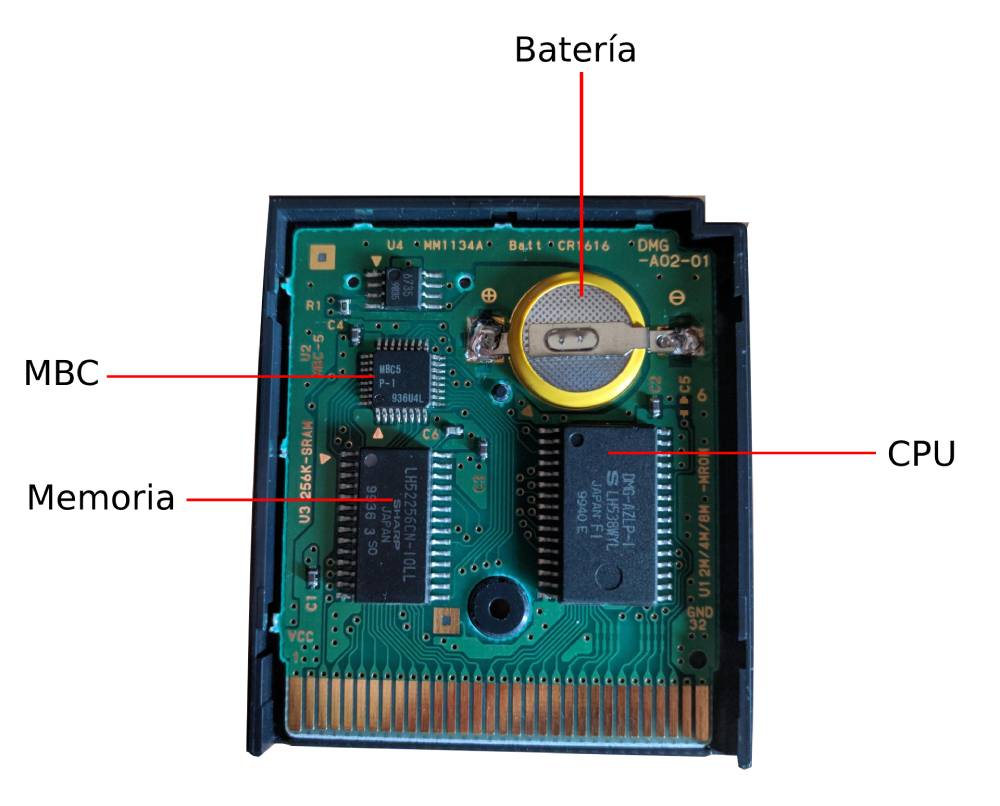
\includegraphics[width=0.7\textwidth]{include/images/cart.jpg}
    \caption{Cartucho de Game Boy MBC5}
    \label{figure:cart_gameboy}
\end{figure}

\subsection{No MBC: 0x00} Los juegos pequeños, que tienen un tamaño de ROM de hasta 32 KiB, no necesitan un utilizar bancos de memoria. En su lugar, la ROM se coloca directamente en la memoria en el rango de direcciones 0x0000-0x7FFF. Además, si se requiere RAM adicional (hasta 8 KiB), se puede conectar en el rango 0xA000-0xBFFF utilizando un circuito lógico.

\subsection{MBC1: 0x01-0x03} Es el modelo de chip más antiguo. Pese a ello, trabaja de forma muy similar a los más recientes, lo que facilitó la actualización de los juegos o la posibilidad de hacerlos retro-compatibles.
\\\\
En la configuración predeterminada (valor 0x00) el MBC1 soporta hasta 512KiB de ROM y un total de 32KiB de RAM mediante el uso de bancos. Esta configuración puede cambiar, por ejemplo para utilizar la parte de RAM como ROM, aumentando esta última hasta 2MiBs. Es importante tener en cuenta que la memoria en el rango de direcciones 0x0000–0x7FFF se usa tanto para leer desde la ROM como para escribir en los registros de control del MBC.

\subsubsection{Memoria}

\paragraph{Banco de ROM 0x00: 0x0000-0x3FFF}
Esta región usualmente contiene los primeros 16KiB de ROM del cartucho (suele ser fija, es decir, no cambia).

\paragraph{Bancos de ROM 0x01-0x7F: 0x4000-0x7FFF}
Esta región puede contener cualquiera de los bancos de 16KiB posibles. La elección del banco se realiza a través del registro 0x2000-0x3FFF.

\paragraph{Banco de RAM 0x00-0x03: 0xA000-0xBFFF}
Esta región se utiliza para leer o escribir en la RAM externa presente en algunos cartuchos (generalmente de tipo 0x02 o 0x03). El acceso a esta RAM solo es posible si está activada mediante la escritura en los registros de control del MBC; de lo contrario, las lecturas devolverán un valor indefinido (comúnmente 0xFF) y las escrituras serán ignoradas.
\\\\
Los tamaños disponibles de RAM son 8 KiB (que cubre toda la región mapeada) o 32 KiB, distribuidos en 4 bancos de 8 KiB cada uno. La segunda opción solo está disponible en cartuchos con ROM de hasta 512 KiB.
\\\\
La RAM externa suele estar alimentada por una batería, lo que permite el almacenamiento de datos incluso cuando la consola está apagada. Esta batería, normalmente una celda de botón soldada en la placa del cartucho, garantiza la persistencia de los datos. Además, dado que la velocidad de la RAM externa es comparable a la RAM interna de la Game Boy, algunos desarrolladores la utilizan como memoria de trabajo adicional (WRAM), aunque esto puede limitar el espacio disponible para el almacenamiento de datos.

\cleardoublepage

\chapter{Metodología y Planificación}
\label{planificacion}

Este capítulo presenta la \textbf{metodología seguida para el desarrollo del proyecto}, así como la \textbf{planificación temporal y técnica}. En primer lugar, se expone el enfoque metodológico adoptado, justificando su idoneidad según el tipo de proyecto y sus objetivos. A continuación, se detallan las distintas etapas en las que se ha estructurado el desarrollo, desde la fase inicial de planificación hasta los resultados y conclusiones.
\\\\
También se hace referencia al concepto de \textbf{Mínimo Producto Viable}, fundamental para \textbf{establecer} una \textbf{primera versión funcional} del emulador que pueda ejecutarse y evaluarse con éxito. Por último, se describen las \textbf{herramientas empleadas} a lo largo del proyecto para el desarrollo de la aplicación.

\section{Metodología Aplicada}
La \textbf{metodología} adoptada para la planificación del proyecto es \textbf{ágil}, un enfoque que, si bien es comúnmente utilizado en proyectos colaborativos, resulta igualmente \textbf{eficaz en proyectos individuales}. La clave de esta metodología radica en la \textbf{gestión eficiente del tiempo}, permitiendo que cada tarea sea ejecutada dentro de un plazo bien definido, con el objetivo de maximizar los resultados y cumplir con los plazos establecidos.

\section{Etapas del Proyecto}
El proyecto está \textbf{dividido en distintas etapas} o iteraciones, cada una de las cuales ofrece la oportunidad de aprender y aplicar nuevos conocimientos relacionados con la emulación y el desarrollo. \textbf{Al final de cada iteración}, se lleva a cabo una \textbf{revisión} exhaustiva del progreso, lo que permite \textbf{identificar áreas de mejora o posibles errores}, minimizando así el tiempo perdido en futuras fases del desarrollo.
\\\\
Durante el proceso de desarrollo, las \textbf{tareas y objetivos} están en \textbf{constante evolución}, dado que se parte de una base de conocimientos limitada que se incrementa a medida que avanza el proyecto. Este enfoque implica que, en muchas ocasiones, lo que en un inicio parecía correctamente implementado debe ser revisado o incluso reestructurado, conforme se adquiere una comprensión más profunda de los desafíos técnicos involucrados.
\\\\
En la \textbf{siguiente tabla} se puede ver la \textbf{planificación estimada} con la que se pretende presentar y defender el proyecto a inicios de Junio de 2024 (C3). \textbf{No se tienen en cuenta posibles retrasos} por enfermedades, viajes u otros.

\begin{table}[H]
    \centering
    \begin{tabular}{|l|l|l|}
    \hline
    \textbf{Apartado} & \textbf{Tiempo estimado} & \textbf{Fecha límite} \\ \hline
    Agradecimientos, Objetivos y Justificación & 1 semana & 25 Agosto \\ \hline
    Planificación y Metodología & 2 semanas & 8 Septiembre \\ \hline
    Diseño & 4 semanas & 6 Octubre \\ \hline
    Aprendizaje & 1 semana & 13 Octubre \\ \hline
    Marco teórico & 3 semanas & 3 Noviembre \\ \hline
    Desarrollo & 5 semanas & 8 Diciembre \\ \hline
    Pruebas y validación & 2 semanas & 22 Diciembre \\ \hline
    Resultados & 1 semana & 29 Diciembre \\ \hline
    Conclusiones y trabajo futuro & 1 semana & 5 Enero \\ \hline
    Bibliografía y Referencias & 1 semana & 12 Enero \\ \hline
    \end{tabular}
    \caption{Planificación de contenidos y fechas límite}
\end{table}

Entrando en detalle en algunas etapas del proeycto:

\begin{itemize}
	\item \textbf{Diseño:} Antes de iniciar el desarrollo del emulador, es fundamental \textbf{tener claros los objetivos y el alcance del proyecto}. Se realizará un \textbf{análisis preliminar} de diversos emuladores existentes, lo cual permitirá obtener una visión más sólida y concreta de las \textbf{funcionalidades y desafíos} que se enfrentarán durante la implementación.

	\item \textbf{Aprendizaje:} En esta fase inicial, el enfoque será \textbf{comprender} en profundidad las \textbf{especificaciones técnicas} de la consola Game Boy, desde su CPU y PPU hasta la gestión de ciclos y sus interacciones con los componentes de hardware. Se realizarán \textbf{pruebas exploratorias}, cuyo propósito será construir una base sólida para el desarrollo posterior del emulador.
	
	\item \textbf{Desarrollo:} Esta es la \textbf{etapa central y más intensiva} del proyecto. Durante el desarrollo del emulador, se \textbf{implementarán las funcionalidades principales} como la emulación de la CPU, la gestión de gráficos, la sincronización de ciclos, y la integración con las interfaces gráficas en Android. Al mismo tiempo, se \textbf{generará la documentación técnica} detallada para acompañar el progreso y justificar las decisiones tomadas durante la implementación.
	
	\item \textbf{Revisión y Maquetación:} La fase final se centrará en la \textbf{revisión exhaustiva} tanto del emulador como de la documentación. Se \textbf{corregirán posibles errores} detectados, se \textbf{optimizará el rendimiento} del emulador, y se \textbf{pulirá la maquetación de la memoria}, asegurando que todo el trabajo cumpla con los estándares de calidad requeridos.
	
\end{itemize}
	
\section{Mínimo Producto Viable}

Lo normal en todo proyecto es que \textbf{ocurran imprevistos} que hagan al programador \textbf{perder más tiempo} en una tarea o incluso \textbf{paralizar por completo el proyecto}. Además, esto se junta con el hecho de que aquí no hay nadie que pueda ocupar nuestro puesto mientras ese problema se soluciona. Por esta razón, es importante tener en mente un \textbf{producto mínimo viable}, con el cual obtener un producto usable de en el tiempo disponible.

\section{Herramientas utilizadas}

El desarrollo de la aplicación se apoyará del uso de las siguientes tecnologías:

\begin{itemize}
    \item \textbf{Android Studio:} Se utilizará como editor de código principal, permitiendo la creación, prueba y depuración de la aplicación mediante emuladores de dispositivos Android.
    \item \textbf{Visual Studio Code:} Herramienta clave para la redacción y visualización de documentos en LaTeX, además de proporcionar un entorno gráfico para gestionar el control de versiones mediante Git.
    \item \textbf{Photoshop:} Herramienta principal de diseño utilizada para la creación de la interfaz gráfica de la aplicación.
    \item \textbf{Procreate:} Aplicación de diseño gráfico que se empleará para la creación de ilustraciones y recursos visuales específicos de la interfaz, complementando a Photoshop en tareas artísticas y detalladas.
\end{itemize}

\begin{figure}[H]
    \centering
    
\includegraphics[width=0.7\textwidth]{include/images/herramientas.png}
    \caption{Herramientas utilizadas en el proyecto}
    \label{figure:tools}
\end{figure}
	
\cleardoublepage
\chapter{Revisión del Mercado de Aplicaciones}
\label{chap:mercado}

Antes de abordar el desarrollo del emulador, resulta fundamental analizar el panorama actual de aplicaciones similares disponibles en el mercado. Este capítulo tiene como objetivo estudiar y comparar distintas soluciones existentes que permiten emular juegos de Game Boy en dispositivos Android, identificando sus características, puntos fuertes y limitaciones.
\\\\
La revisión se centra en emuladores reconocidos como My OldBoy! y GBCC, prestando especial atención a aspectos como el rendimiento, la interfaz de usuario, las opciones de configuración y el sistema de monetización.
\\\\
Este análisis no solo proporciona una visión general del estado de la tecnología en este ámbito, sino que también permite identificar oportunidades de mejora y justificar las decisiones de diseño adoptadas en el presente proyecto.

\section{Referencias}
En esta sección se encuentran aquellas aplicaciones que, tras una revisión de los mismos, se cree que han sido de utilidad por su parecido a la hora de desarrollar este proyecto:

\subsubsection{My OldBoy!}

\textbf{My OldBoy!} es un emulador de Game Boy y Game Boy Color diseñado específicamente para dispositivos Android, que destaca por su precisión en la emulación de casi todos los aspectos del hardware original. Además de simular las consolas, soporta características especiales como el uso del cable link, la vibración y el sensor de inclinación.
\\\\
El emulador es altamente valorado por su interfaz intuitiva y las múltiples opciones de personalización, que incluyen la posibilidad de añadir colores a juegos monocromáticos y modificar la disposición y el tamaño de los controles en pantalla. Entre las ventajas que ofrece, están la alta compatibilidad con juegos y la capacidad de ajustar la velocidad del juego, tanto para avanzar rápidamente como para ralentizarlo en momentos difíciles.
\\\\
Sin embargo, tiene algunas limitaciones. Por ejemplo, puede generar archivos de guardado duplicados, carece de un sistema de autoguardado periódico y no ha recibido actualizaciones recientes para las versiones más nuevas de Android, lo que puede afectar su compatibilidad en dispositivos más modernos.

\clearpage

\begin{figure}[h]
    \centering
    
\includegraphics[width=0.25\textwidth]{include/images/myoldboy.png}
    \caption{My OldBoy! - Logotipo.}
    \label{figure:oldboylogo}
\end{figure}

La pantalla principal de la aplicación presenta un explorador de archivos que muestra, en formato de lista, los documentos almacenados en la carpeta especificada de la memoria interna del dispositivo. Los archivos se organizan automáticamente por orden alfabético, ofreciendo una visualización clara y estructurada para facilitar su navegación y selección. Dispone de dos botones, uno para recargar la carpeta actual y otro para acceder a los ajustes de sistema. 
\\\\
En los ajustes, podremos modificar distintos aspectos agrupados en las categorías de video, audio, datos de entrada, disposición, varios y avanzado. En vídeo, por ejemplo, podremos modificar el tamaño de la pantalla de juego, la orientación predeterminada de la aplicación, o la paleta de colores.

\begin{figure}[h]
    \centering
    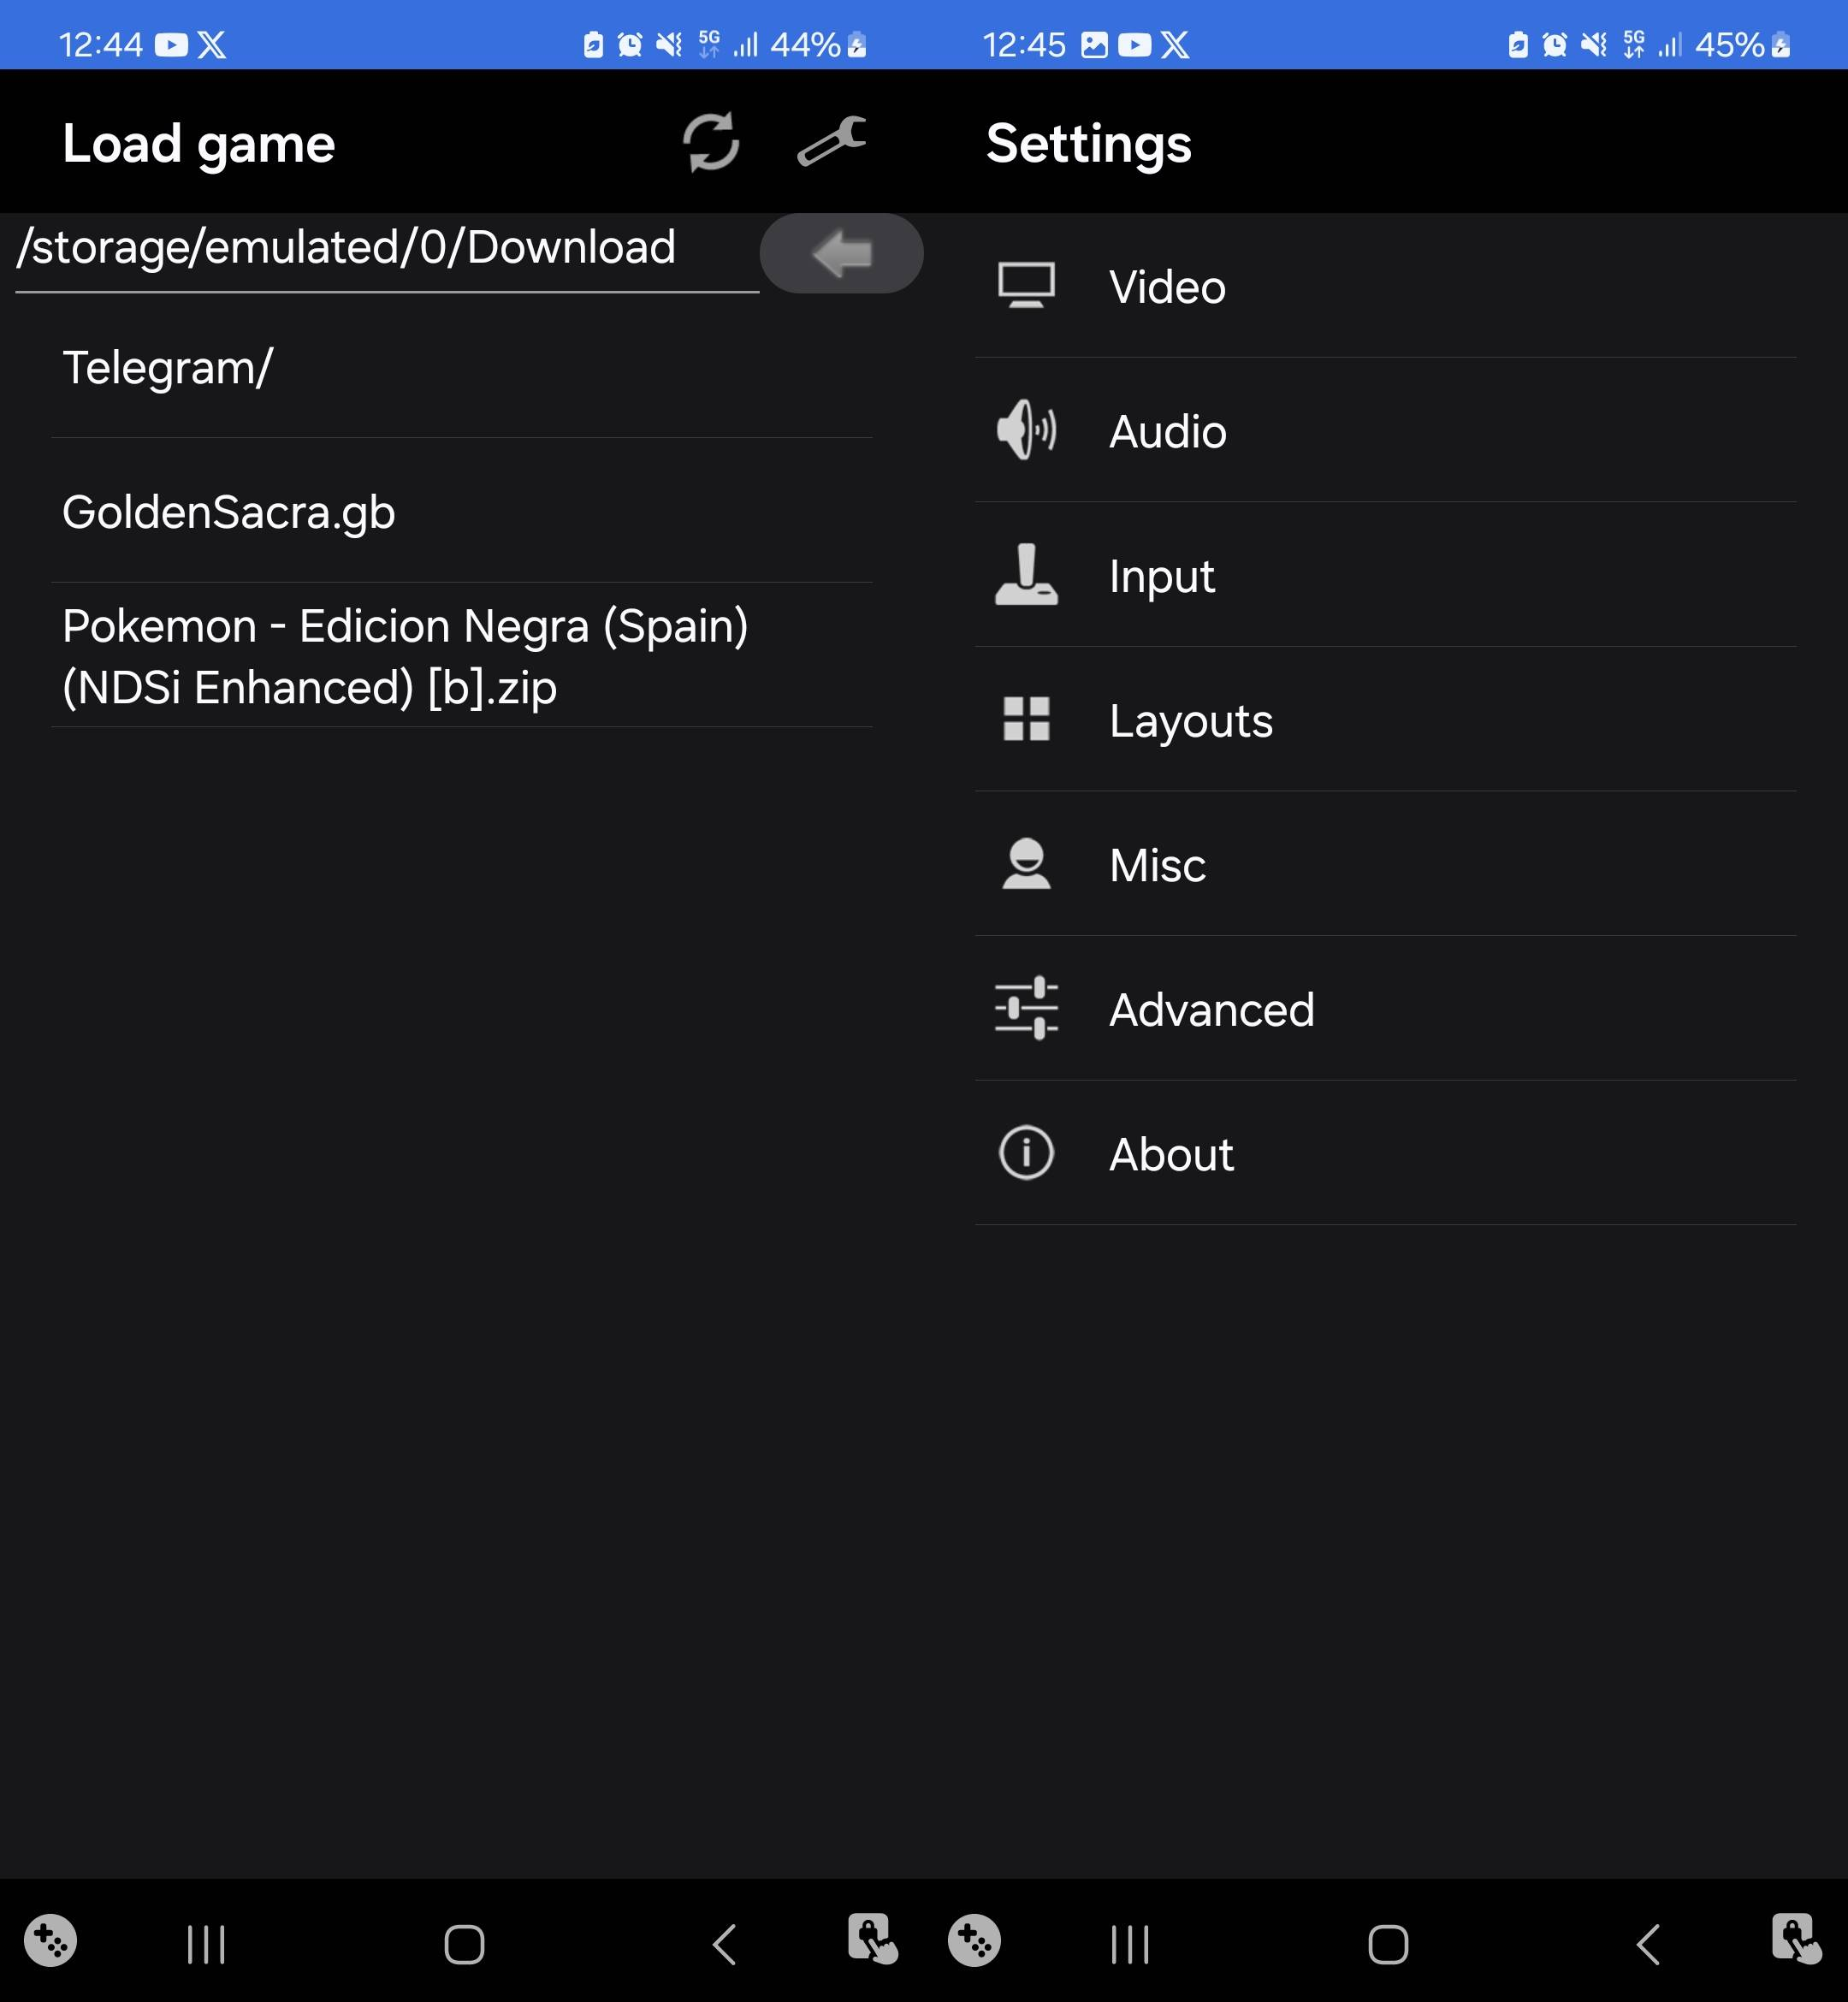
\includegraphics[width=0.55\textwidth]{include/images/myoldboy2.jpg}
    \caption{My OldBoy! - Menú de inicio y pantalla de ajustes.}
    \label{figure:oldboy2}
\end{figure}

\clearpage

La pantalla de juego presenta un diseño más simplificado en comparación con otros emuladores destacados. Su principal ventaja radica en la facilidad para ajustar la posición y tamaño de los botones, permitiendo al usuario personalizar su experiencia de juego. Sin embargo, algunos usuarios consideran que, dado que se trata de una aplicación de pago, el aspecto gráfico podría beneficiarse de mejoras adicionales para estar a la altura de sus competidores.

\begin{figure}[h]
    \centering
    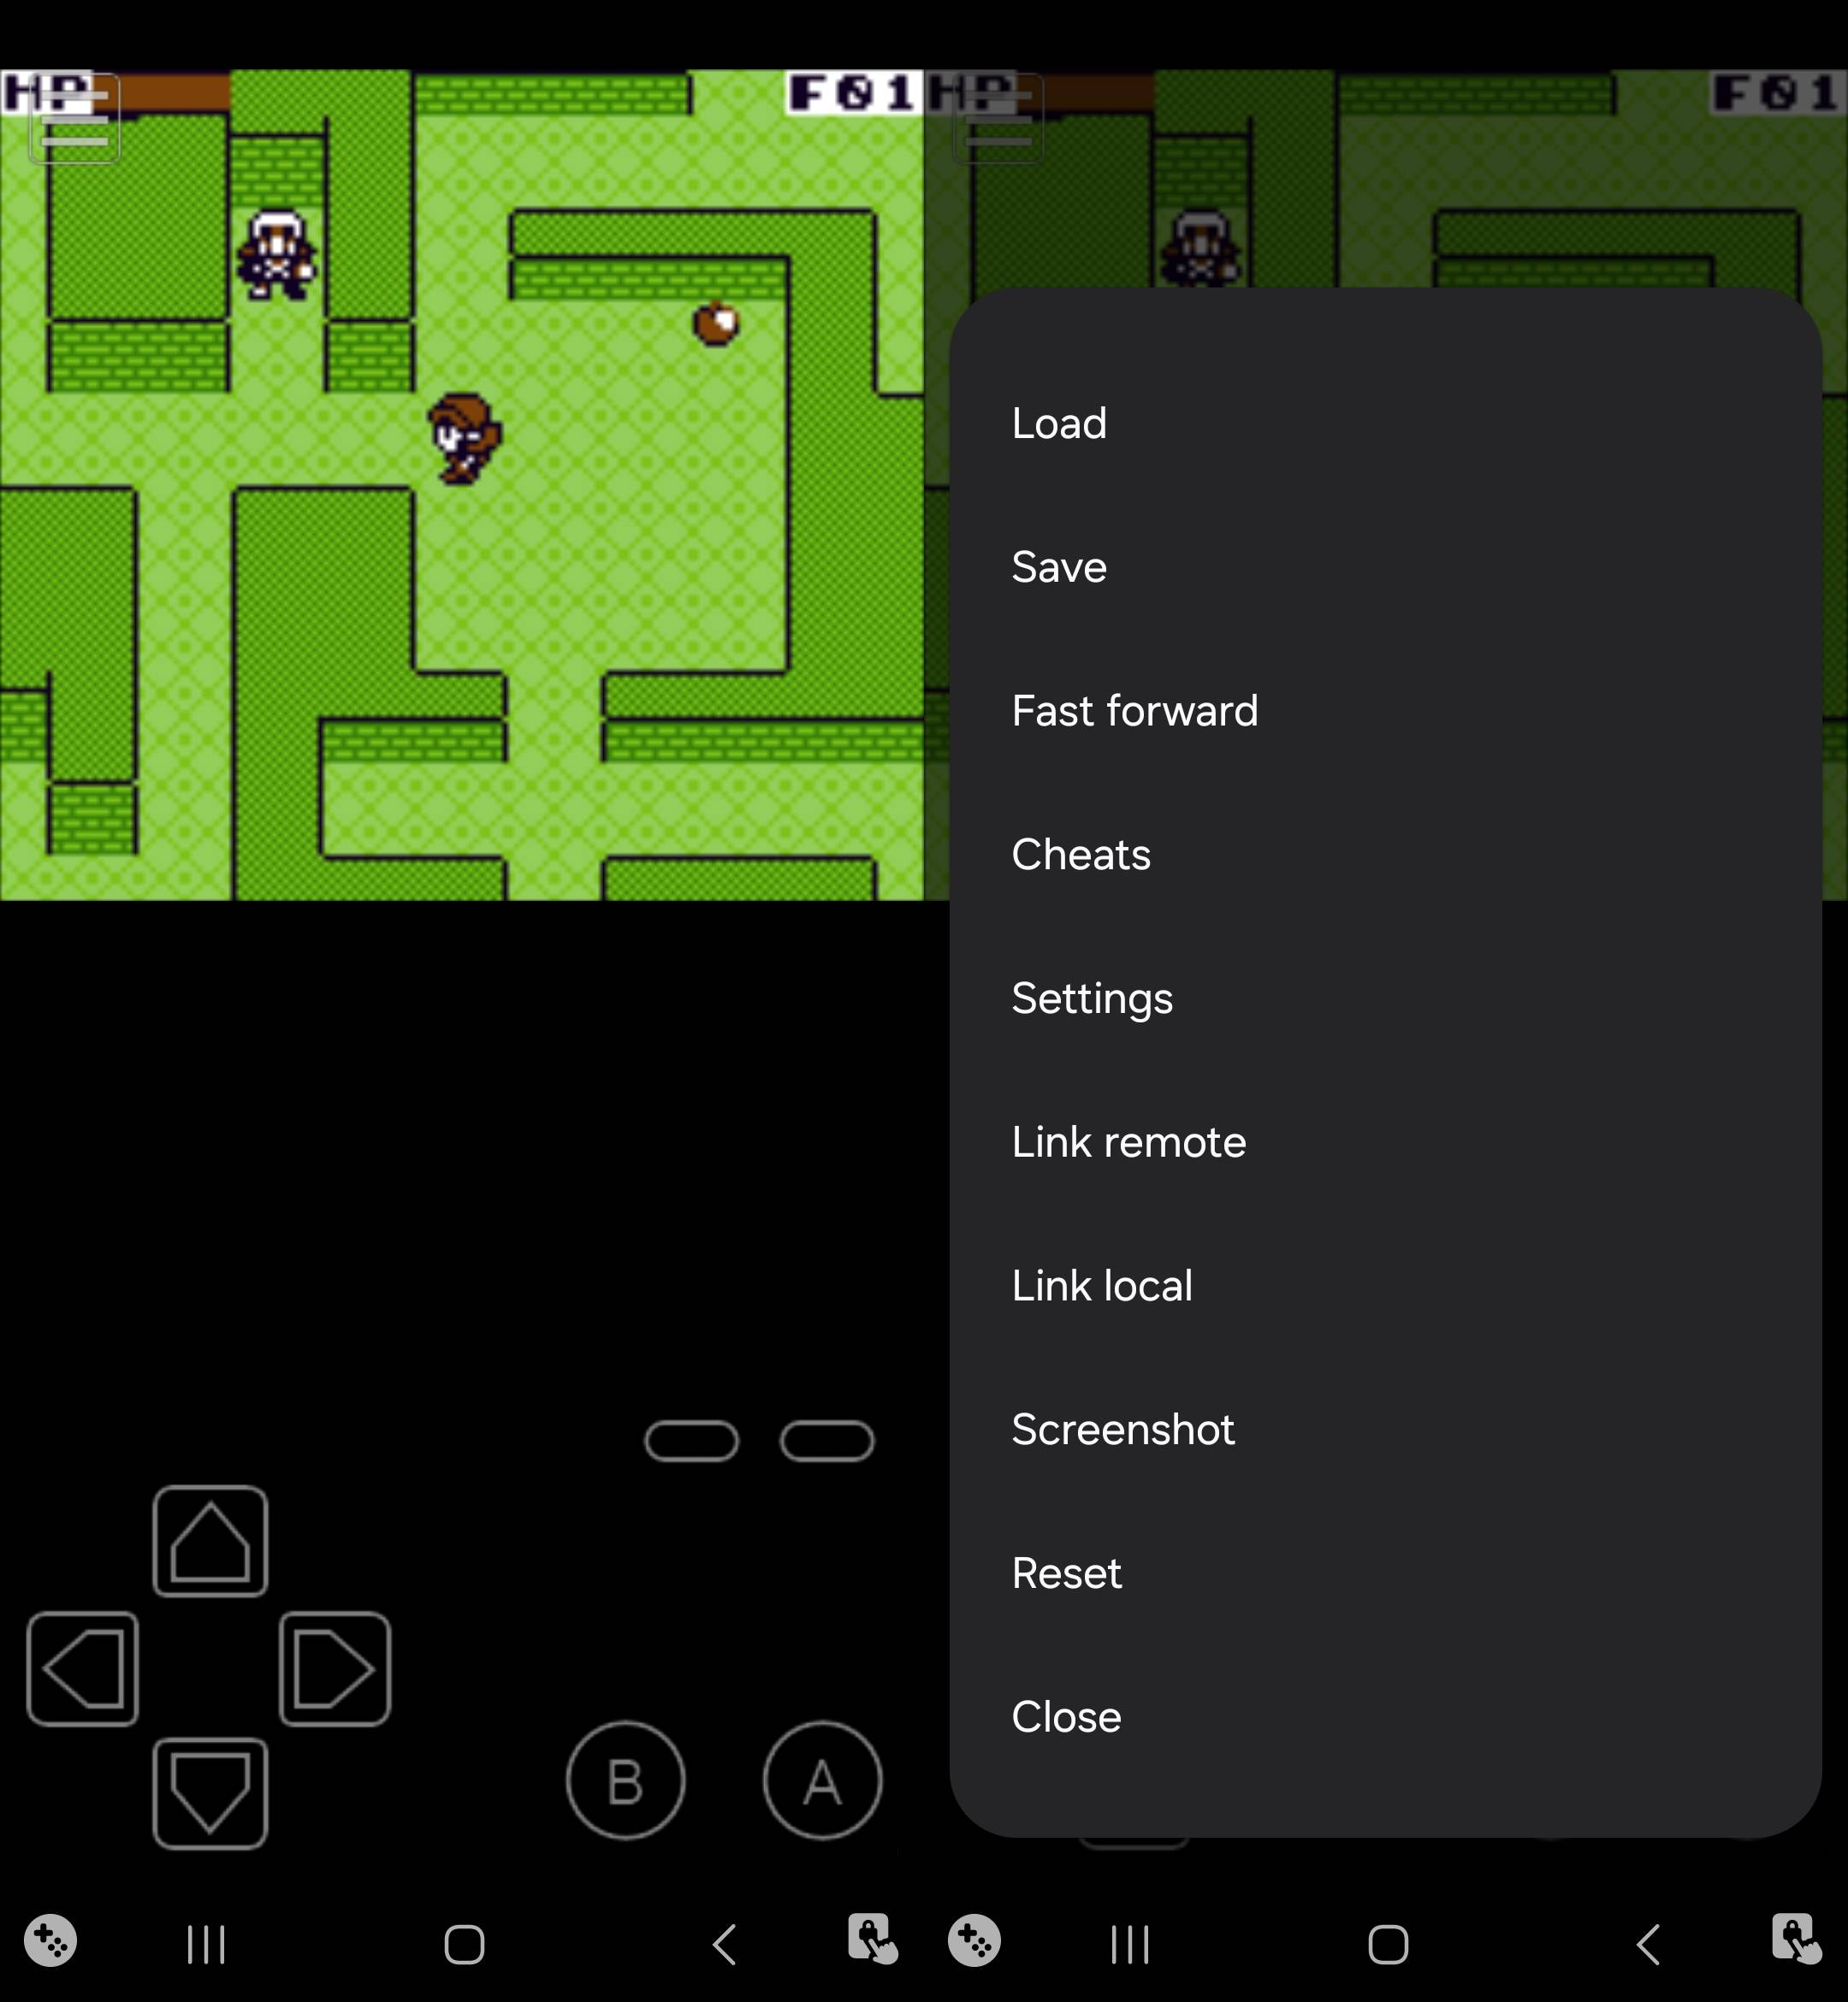
\includegraphics[width=0.65\textwidth]{include/images/myoldboy3.jpg}
    \caption{My OldBoy! - Pantalla y opciones de juego.}
    \label{figure:oldboy3}
\end{figure}
\begin{figure}[H]
    \centering
    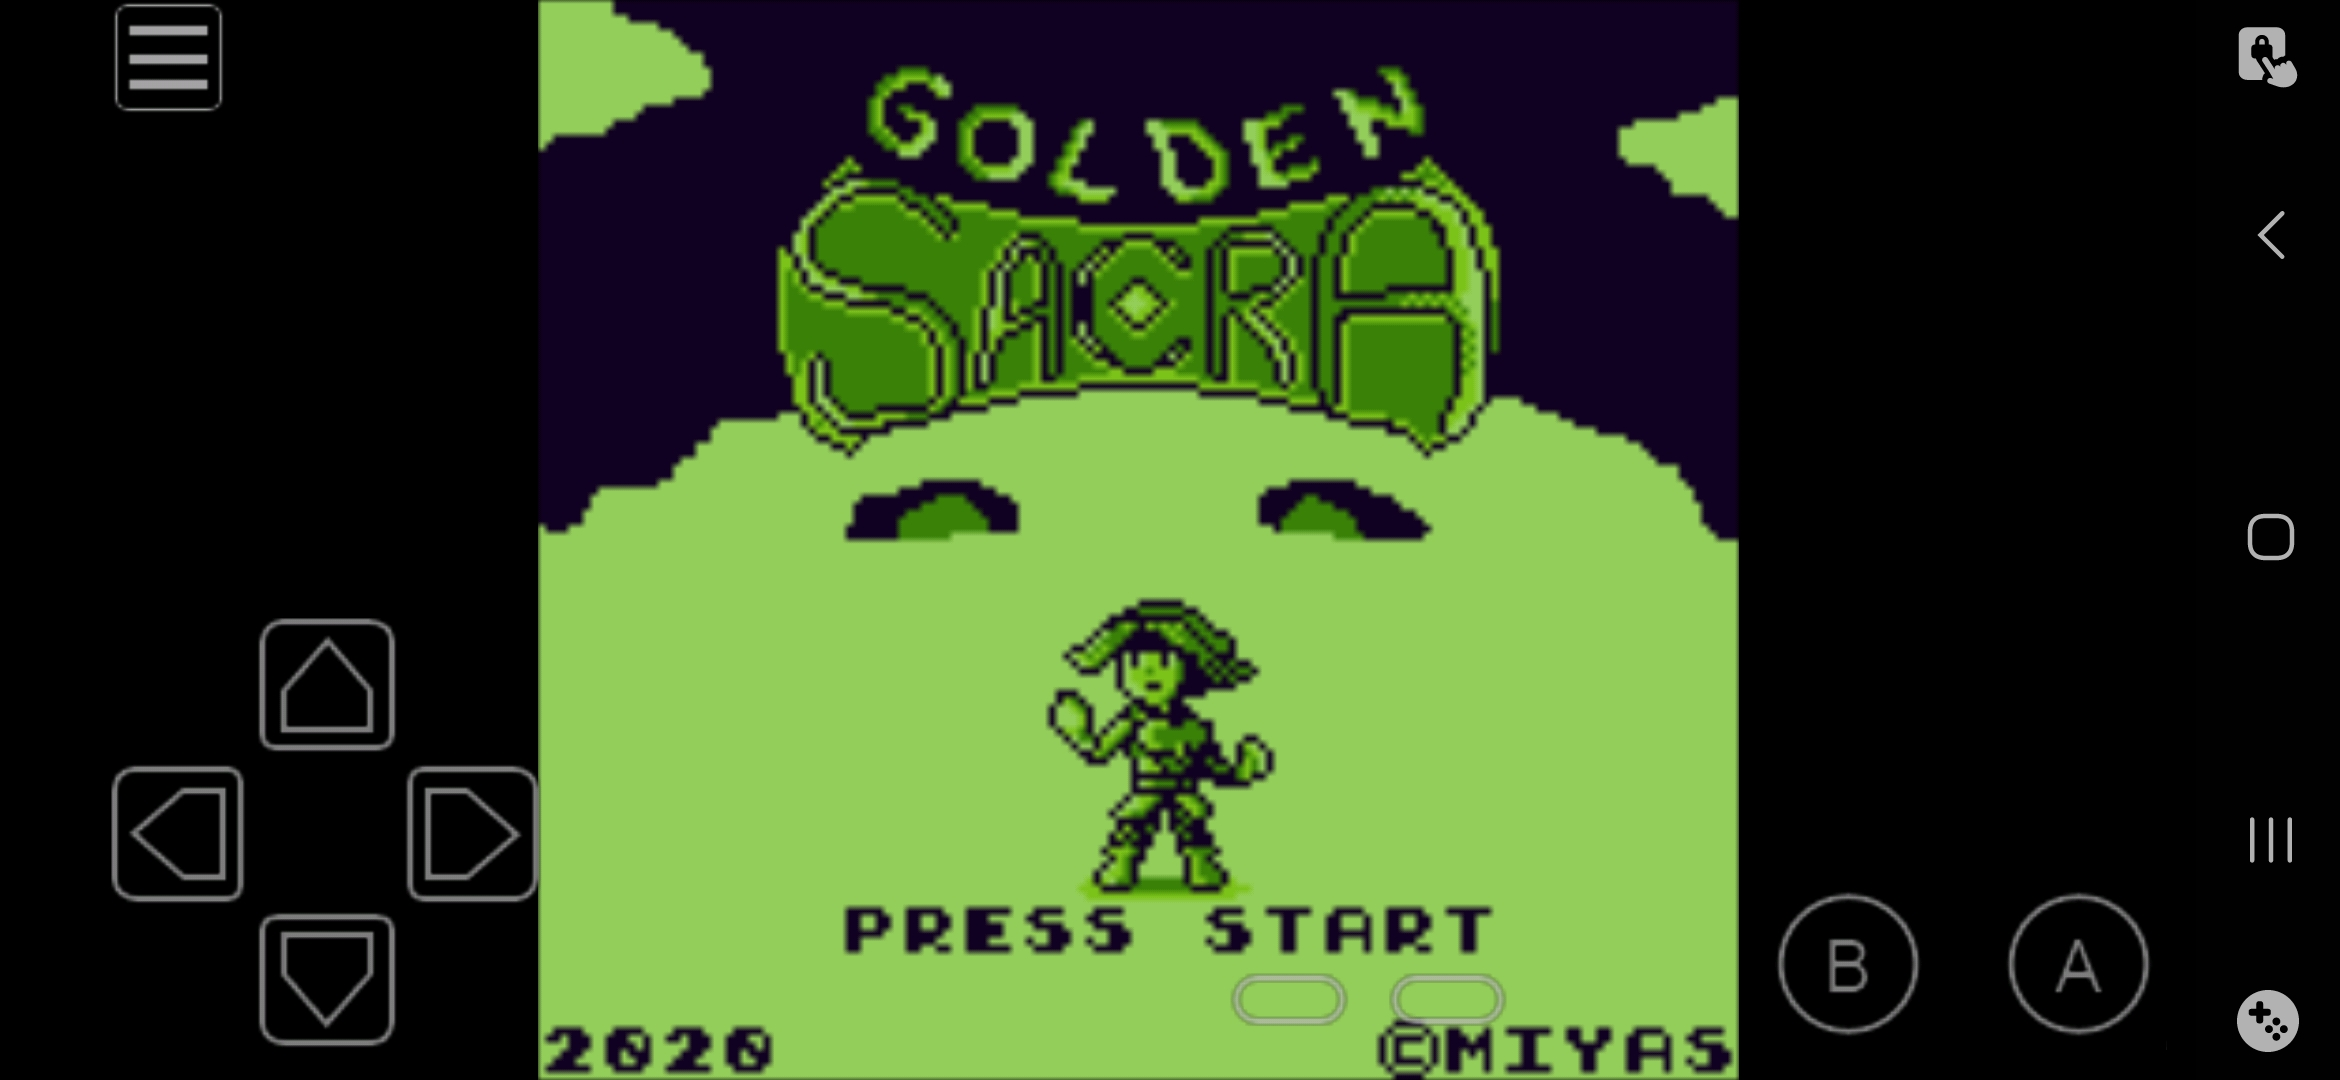
\includegraphics[width=0.65\textwidth]{include/images/myoldboyportrait.jpg}
    \caption{My OldBoy! - Pantalla de juego en orientación horizontal.}
    \label{figure:oldboy4}
\end{figure}

\clearpage

\subsubsection{GBCC}
GBCC es un emulador multiplataforma de Game Boy y Game Boy Color desarrollado en lenguaje C. Está disponible en Linux, Windows, Android y macOS.
\\\\
Entre sus funcionalidades se incluyen soporte para GUIs basadas en SDL y GTK, paletas personalizadas para juegos DMG, estados de guardado automáticos, y una función de turbo ajustable. También soporta shaders como Dot-Matrix y Subpixel, los cuales permiten una reproducción precisa de los colores en CGB. Además, ofrece integración con hardware como el Rumble Pak, acelerómetros y la Game Boy Printer, aunque algunos periféricos como el IR Port y el Pocket Sonar no están implementados.
\\\\
También soporta diversos controladores de memoria: MBC1, MBC2, MBC3 y MBC5, pero aún carece de soporte para MBC6 y MBC7, entre otros. Además, el emulador tiene la capacidad de simular el cable link, aunque es una conexión \textit{fake} consigo mismo.
\\\\
El proyecto se destaca por su compatibilidad con shaders y la posibilidad de visualizar los datos de VRAM en una ventana separada, lo cual es útil para desarrolladores y aficionados que quieran inspeccionar los gráficos en detalle.

\begin{figure}[h]
    \centering
    
\includegraphics[width=0.6\textwidth]{include/images/gbcclogo.png}
    \caption{GBCC - Logotipo.}
    \label{figure:gbcclogo}
\end{figure}

La pantalla de juego se caracteriza por su diseño minimalista y adaptable. Dependiendo de si se carga una ROM de Game Boy (DMG) o de Game Boy Color (CGB), la interfaz ajusta su apariencia para emular de manera más fiel las características visuales de la consola correspondiente. El diseño de los controles también se adapta dinámicamente a las dimensiones del dispositivo: en modo vertical, la separación entre los botones y la escala de la pantalla gráfica varían según el ancho y el alto disponibles. En el modo horizontal, el diseño se ajusta automáticamente, manteniendo la proporción y los colores, sin perder la coherencia visual. Además, se pueden observar características adicionales como el botón de turbo y la aplicación de shaders como el Dot-Matrix para mejorar la experiencia visual.
\\\\
Por último, GBCC permite personalizar el fondo de pantalla que simula la consola original, brindando la opción de cambiar el color según las preferencias del usuario, lo que añade un toque personal a la experiencia de emulación. Esta característica es muy apreciada por quienes buscan una mayor personalización en la interfaz.

\begin{figure}[h]
    \centering
    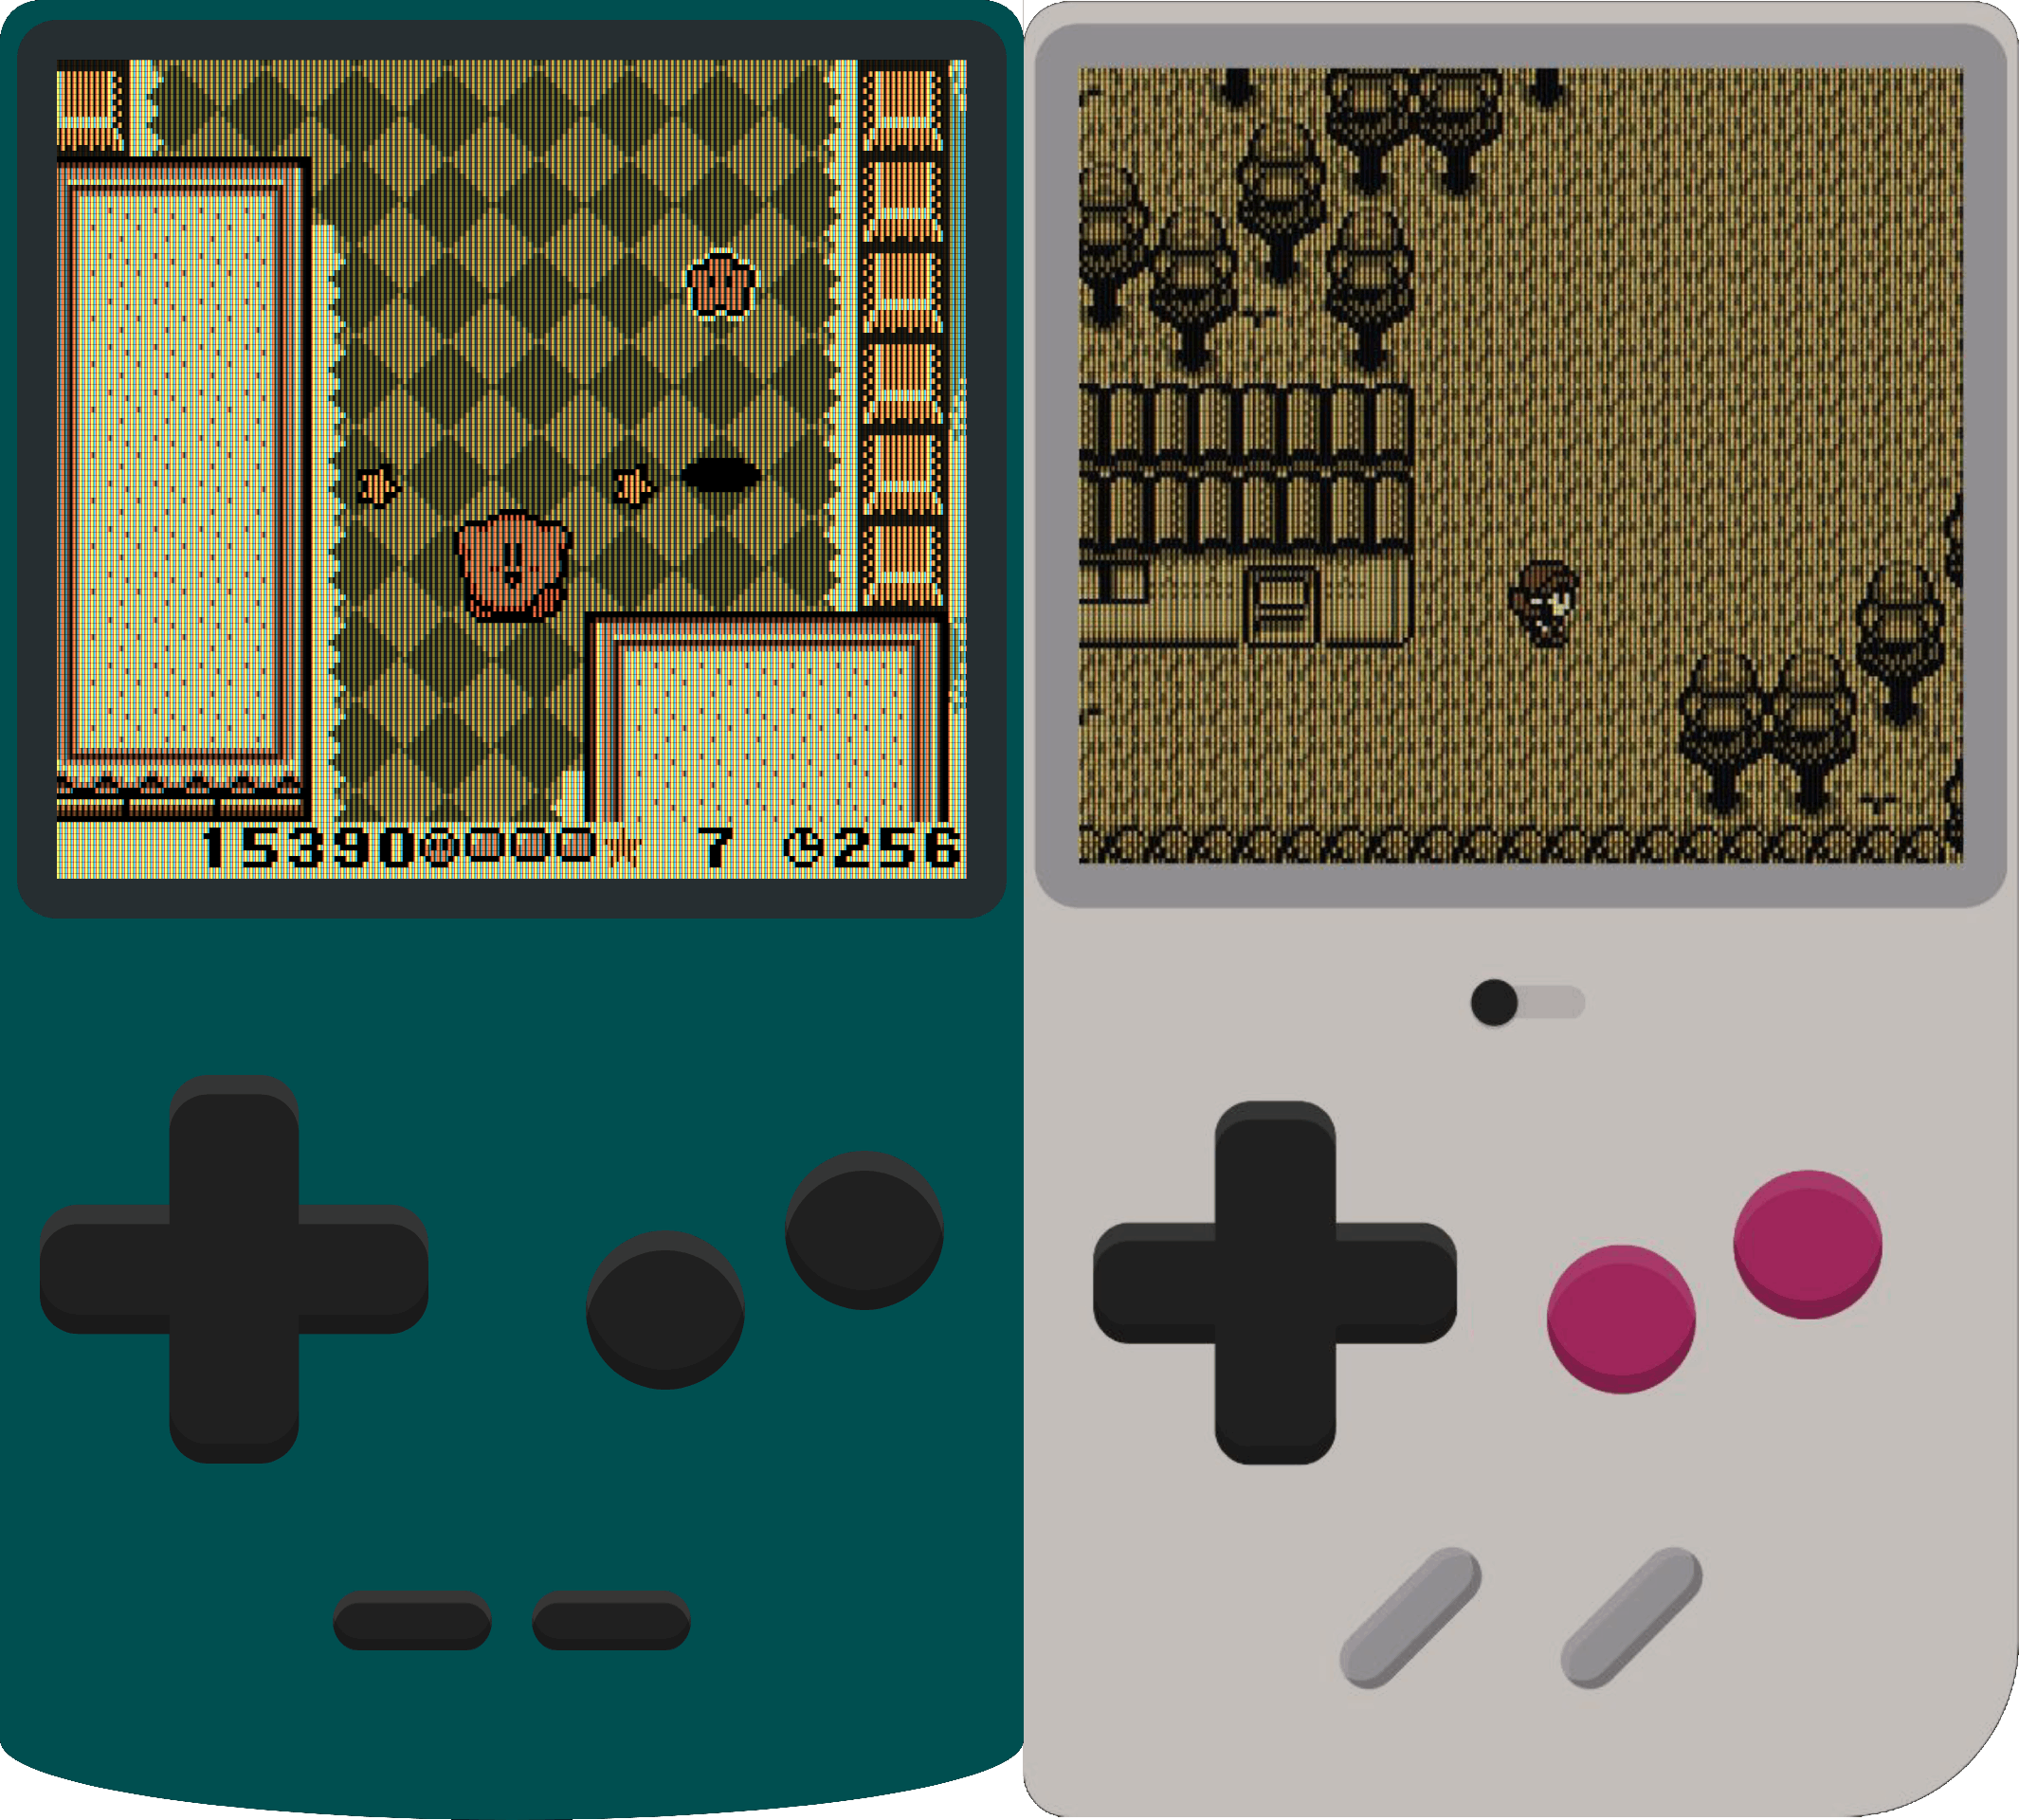
\includegraphics[width=0.6\textwidth]{include/images/gbccgame.png}
    \caption{GBCC - Pantalla de juego.}
    \label{figure:gbccgame}
\end{figure}

\begin{figure}[h]
    \centering
    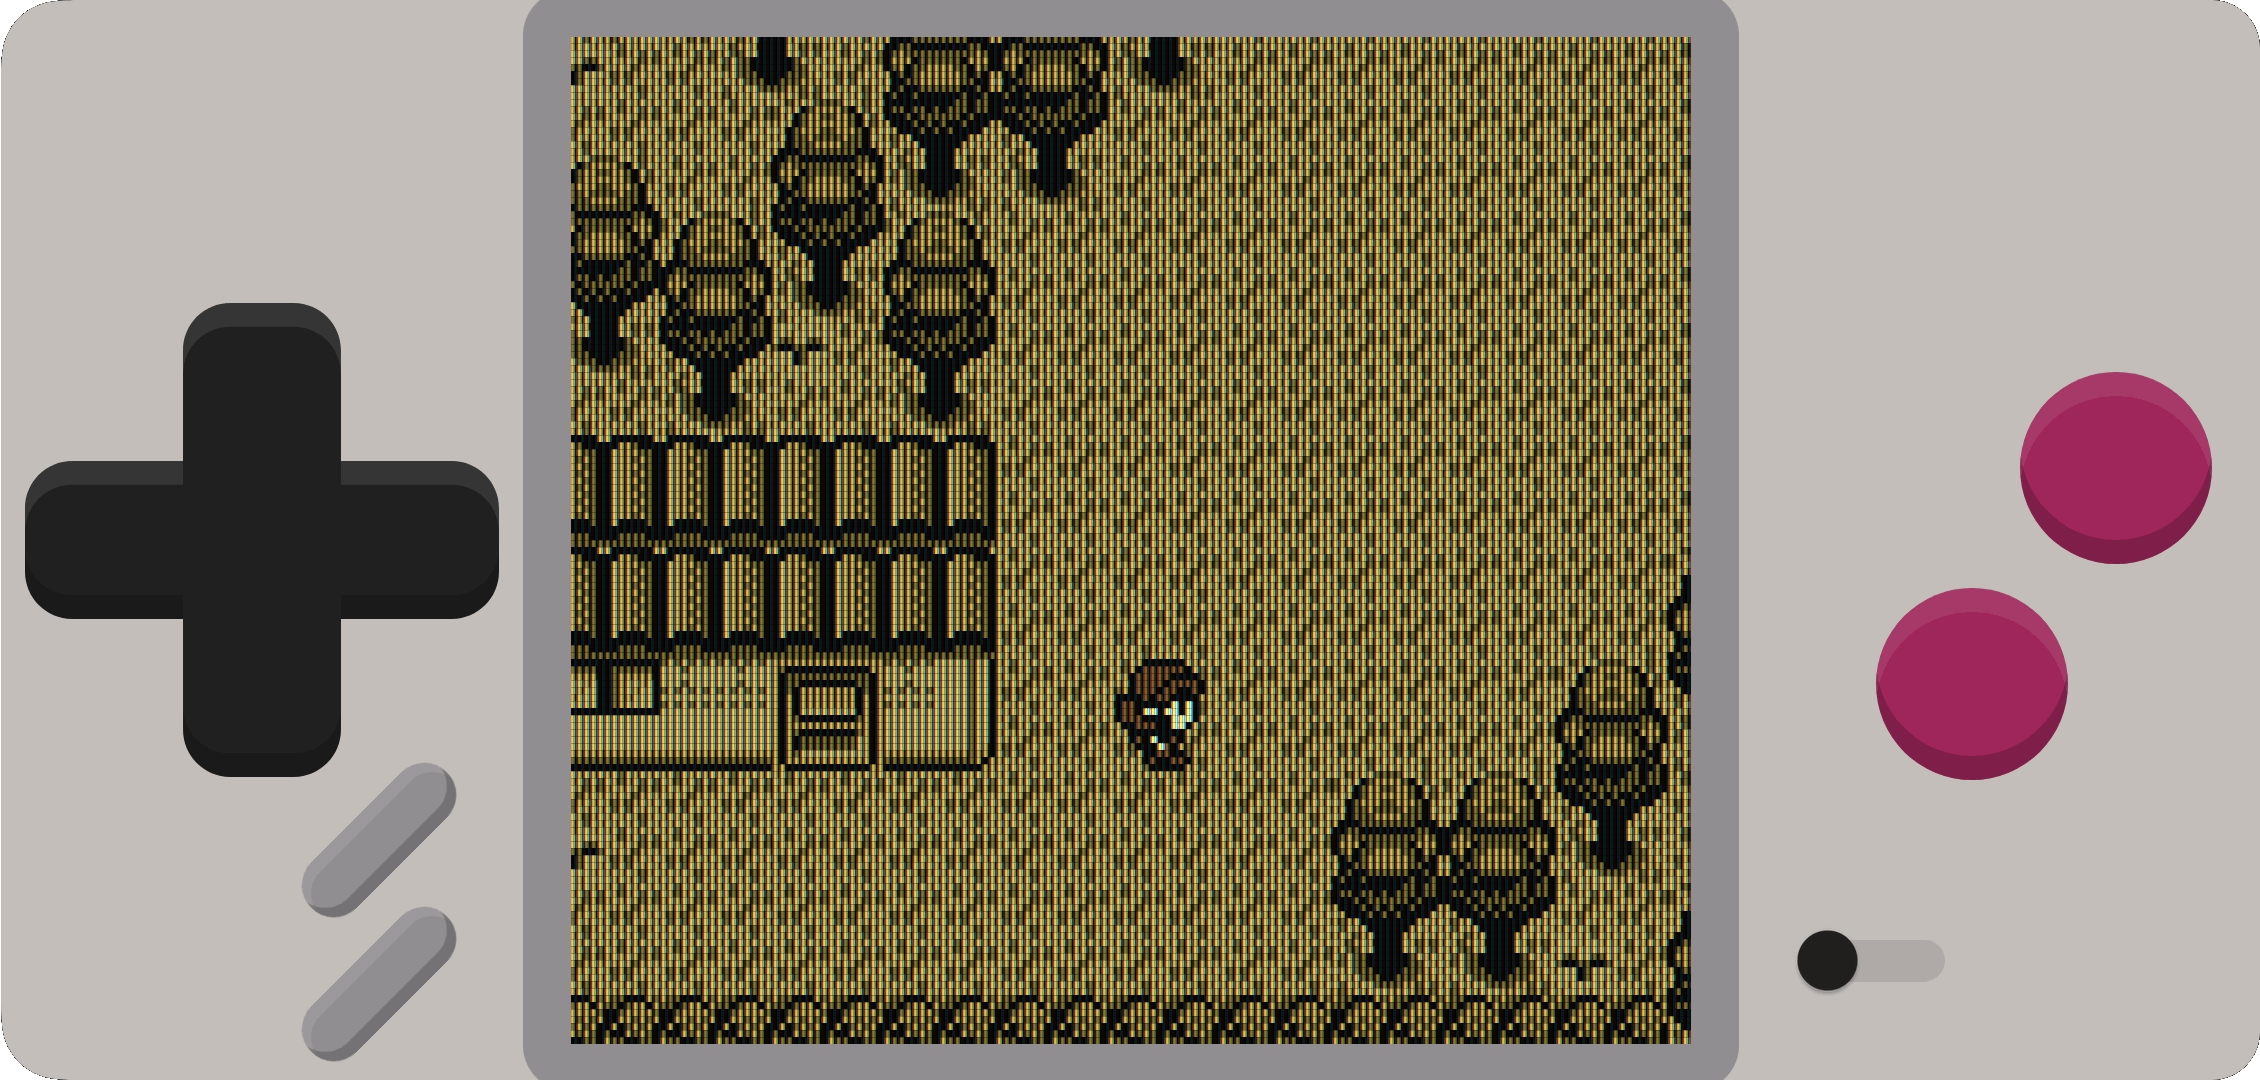
\includegraphics[width=0.6\textwidth]{include/images/gbccgameportrait.png}
    \caption{GBCC - Pantalla de juego en orientación horizontal.}
    \label{figure:gbccgameportrait}
\end{figure}

\clearpage

\subsubsection{iGBA}

El emulador iGBA fue una aplicación diseñada para dispositivos iOS, disponible brevemente en la App Store antes de ser retirada en abril de 2024. Permitía a los usuarios emular juegos de Game Boy, Game Boy Color y Game Boy Advance en sus iPhones, ofreciendo características como guardado de estado, avance rápido y soporte para ROMs legalmente adquiridas.
\\\\
Entre sus características principales destacaban la capacidad de guardar estados de juego, permitiendo a los usuarios guardar y retomar partidas en cualquier momento, además de la función de avance rápido (igual que GBCC), que permitía saltar rápidamente escenas o partes lentas del juego. Sin embargo, un detalle a mejorar era que esta velocidad del avance era excesivamente rápida y no permitía ajustes más finos.

\begin{figure}[h]
    \centering
    
\includegraphics[width=0.3\textwidth]{include/images/igbalogo.png}
    \caption{iGBA - Logotipo.}
    \label{figure:igbalogo}
\end{figure}

La interfaz era sencilla, con un diseño limpio que simulaba los botones de las consolas originales. Sin embargo, generó controversia por dos razones: incluir anuncios que interrumpían la experiencia de juego y ser una copia no autorizada de GBA4iOS, un emulador desarrollado por \textit{Riley Testut}. Este conflicto con el código de GBA4iOS, junto con la preocupación por la privacidad y la recopilación de datos de los usuarios, llevó a críticas dentro de la comunidad de emuladores​.
\\\\
Los controles virtuales incluían botones de hombro para los juegos de Game Boy Advance, aunque algunos usuarios mencionaron que estos botones eran algo pequeños. Además, ofrecía un menú de opciones en la esquina inferior izquierda con funciones como guardado rápido, carga de estados, códigos de trucos y avance rápido.
\\\\
A pesar de sus problemas, algunos usuarios apreciaron lo fácil que era configurarlo y su capacidad para emular juegos retro sin retrasos significativos.

\begin{figure}[h]
    \centering
    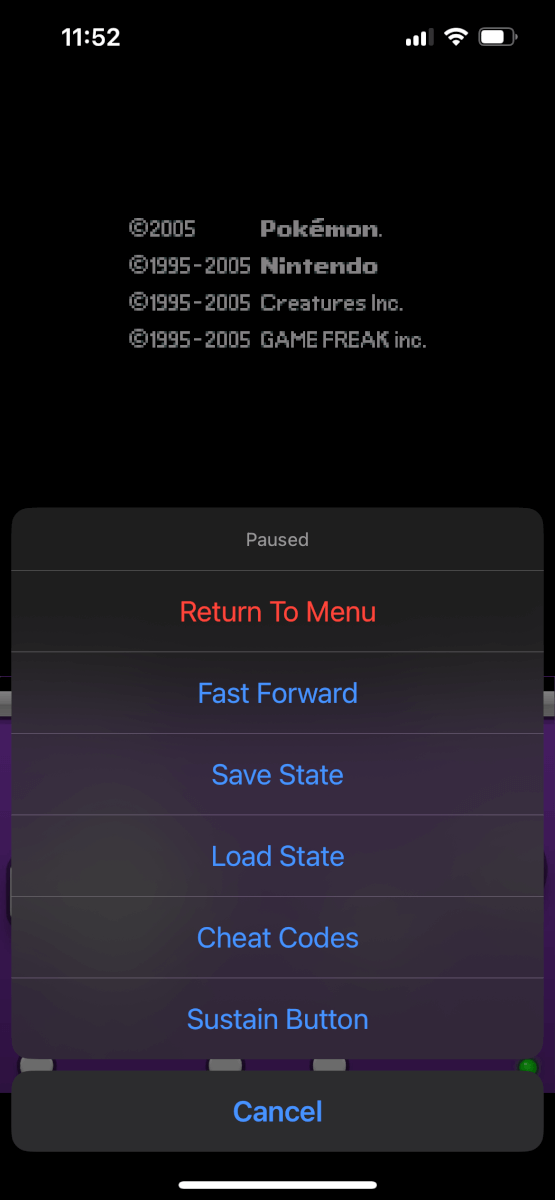
\includegraphics[width=0.25\textwidth]{include/images/igbasettings.PNG}
    \caption{iGBA - Ajustes de juego.}
    \label{figure:igbasettings}
\end{figure}

\begin{figure}[h]
    \centering
    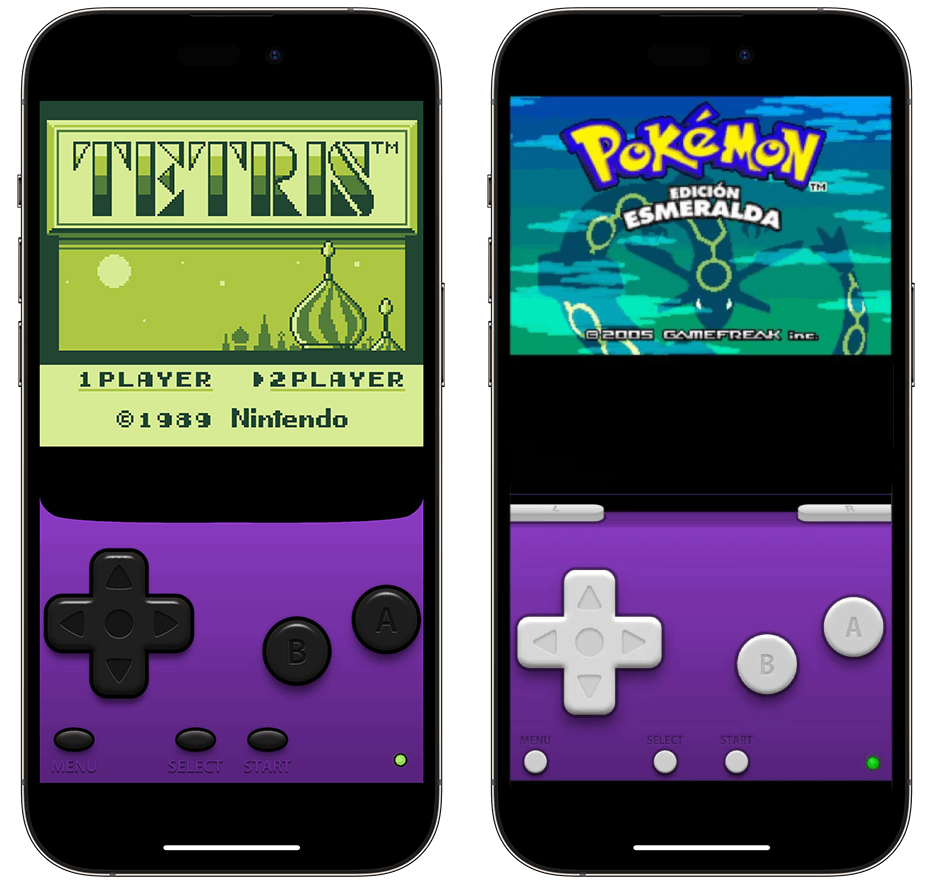
\includegraphics[width=0.65\textwidth]{include/images/iGBAgame.png}
    \caption{iGBA - Pantalla de juego.}
    \label{figure:igbagame}
\end{figure}


\cleardoublepage

\chapter{Análisis y Diseño}
\label{design}

Este capítulo recoge el proceso de análisis y diseño previo al desarrollo del emulador, donde se definen los requisitos que debe cumplir la aplicación y se plantean las primeras decisiones estructurales y visuales del proyecto.
\\\\
En primer lugar, se detallan los requisitos funcionales y no funcionales, los cuales especifican tanto las funcionalidades que debe ofrecer la aplicación como las restricciones de calidad, rendimiento o usabilidad que debe respetar. A continuación, se presentan los casos de uso, acompañados de su correspondiente diagrama, para ilustrar de manera clara la interacción entre el usuario y el sistema.
\\\\
Finalmente, se incluyen una serie de mockups que representan visualmente la interfaz de usuario en sus distintas pantallas, ayudando a anticipar la experiencia del usuario final y facilitando una primera validación del diseño.

\section{Requerimientos}

A continuación se detallan los requerimientos funcionales y no funcionales que rigen el diseño y la implementación del proyecto. Estos requerimientos han sido definidos a partir del análisis de las necesidades del usuario final y de las restricciones técnicas:

\subsection{Requerimientos Funcionales}

Estos requerimientos son las capacidades específicas que la aplicación debe cumplir para garantizar que su funcionamiento sea acorde a los objetivos establecidos:

\begin{itemize}
    \item \textbf{Carga de ROMs}: El usuario debe poder seleccionar y cargar archivos .gb o .gbc desde su dispositivo.
    \item \textbf{Emulación}: Debe replicar fielmente el comportamiento del hardware original.
    \item \textbf{Interfaz táctil}: Proveer botones virtuales que simulen los originales.
    \item \textbf{Audio}: Emular el sonido original de la consola.
    \item \textbf{Gestión de estado}: Guardar y cargar partidas.
    \item \textbf{Compatibilidad}: Dar soporte para ROMs de DMG y CGB.
    \item \textbf{Configuraciones}: Permitir al usuario ajustar las características del emulador, como la velocidad y los controles.
\end{itemize}

\subsection{Requerimientos No Funcionales}

Estos requerimientos se enfocan en aspectos de calidad de la aplicación, como el rendimiento o la usabilidad, con el objetivo de asegurar una experiencia fluida y eficiente.

\begin{itemize}
    \item \textbf{Rendimiento}: La emulación debe ir a la frecuencia original de la consola en la mayoría de los dispositivos Android.
    \item \textbf{Compatibilidad}: Funcionar en dispositivos Android 8.0 o superior.
    \item \textbf{Eficiencia}: Consumo de batería optimizado durante la ejecución.
    \item \textbf{Usabilidad}: La interfaz debe ser intuitiva y accesible para el usuario.
    \item \textbf{Mantenimiento}: Código modular, que sea fácil de escalar y el cual disponga de una buena documentación para facilitar futuras mejoras.
\end{itemize}

\section{Casos de Uso}

Los casos de uso permiten identificar y documentar cómo los usuarios interactuarán con el sistema, destacando las funcionalidades clave y sus flujos de ejecución.

\begin{figure}[H]
    \centering
    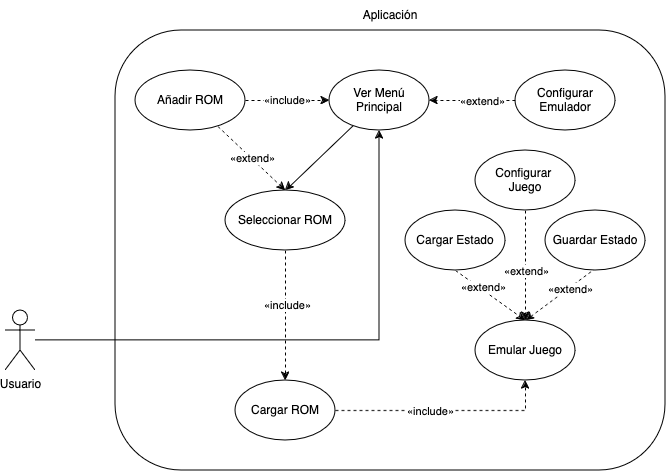
\includegraphics[width=0.7\textwidth]{include/images/casosuso.png}
    \caption{Diagrama de Casos de Uso}
    \label{figure:usecases}
\end{figure}

El usuario tiene acceso directo al menú principal al entrar en la aplicación. Desde ahí, el usuario puede realizar diferentes acciones como añadir o seleccionar una ROM o configurar de forma general el emulador. La selección de una ROM incluye los procesos de carga y emulación. Además, durante la emulación, el usuario puede cargar o guardar el estado y configurar el juego. Las relaciones entre los casos de uso se estructuran con inclusiones para acciones necesarias y extensiones para funcionalidades opcionales.

\section{Mockup}

La aplicación seguirá un diseño minimalista, tomando como referencia principal el emulador GBCC. En su versión inicial, el menú principal presentará una lista en formato de cuadrícula que mostrará todas las ROMs agregadas por el usuario. Cada uno de los elementos de la cuadrícula contará con una imagen predeterminada, representando la consola original, ya sea DMG o CGB, junto con el nombre de la ROM. Estas se ordenarán alfabéticamente para facilitar la navegación. Este enfoque busca mantener una interfaz limpia y funcional, con un acceso directo a los juegos.
\\\\
En la barra de navegación se mostrarán dos íconos. El primero, representado por un símbolo de suma ("+"), permitirá al usuario agregar nuevas ROMs a la aplicación. El segundo ícono, con la forma de un engranaje, brindará acceso a la configuración general del emulador, que incluirá opciones relacionadas con el video, audio, disposición de controles, entre otros. Estas configuraciones tendrán un impacto en todos los juegos de manera uniforme.
\\\\
La imagen de cada juego podrá ser personalizada por el usuario a través de un gesto táctil de "hold". Al realizar este gesto sobre una cuadrícula específica, el usuario tendrá la capacidad de acceder a los ajustes individuales del juego, donde podrá reemplazar la imagen predeterminada por una de su elección o modificar el nombre del juego.

\begin{figure}[h]
    \centering
    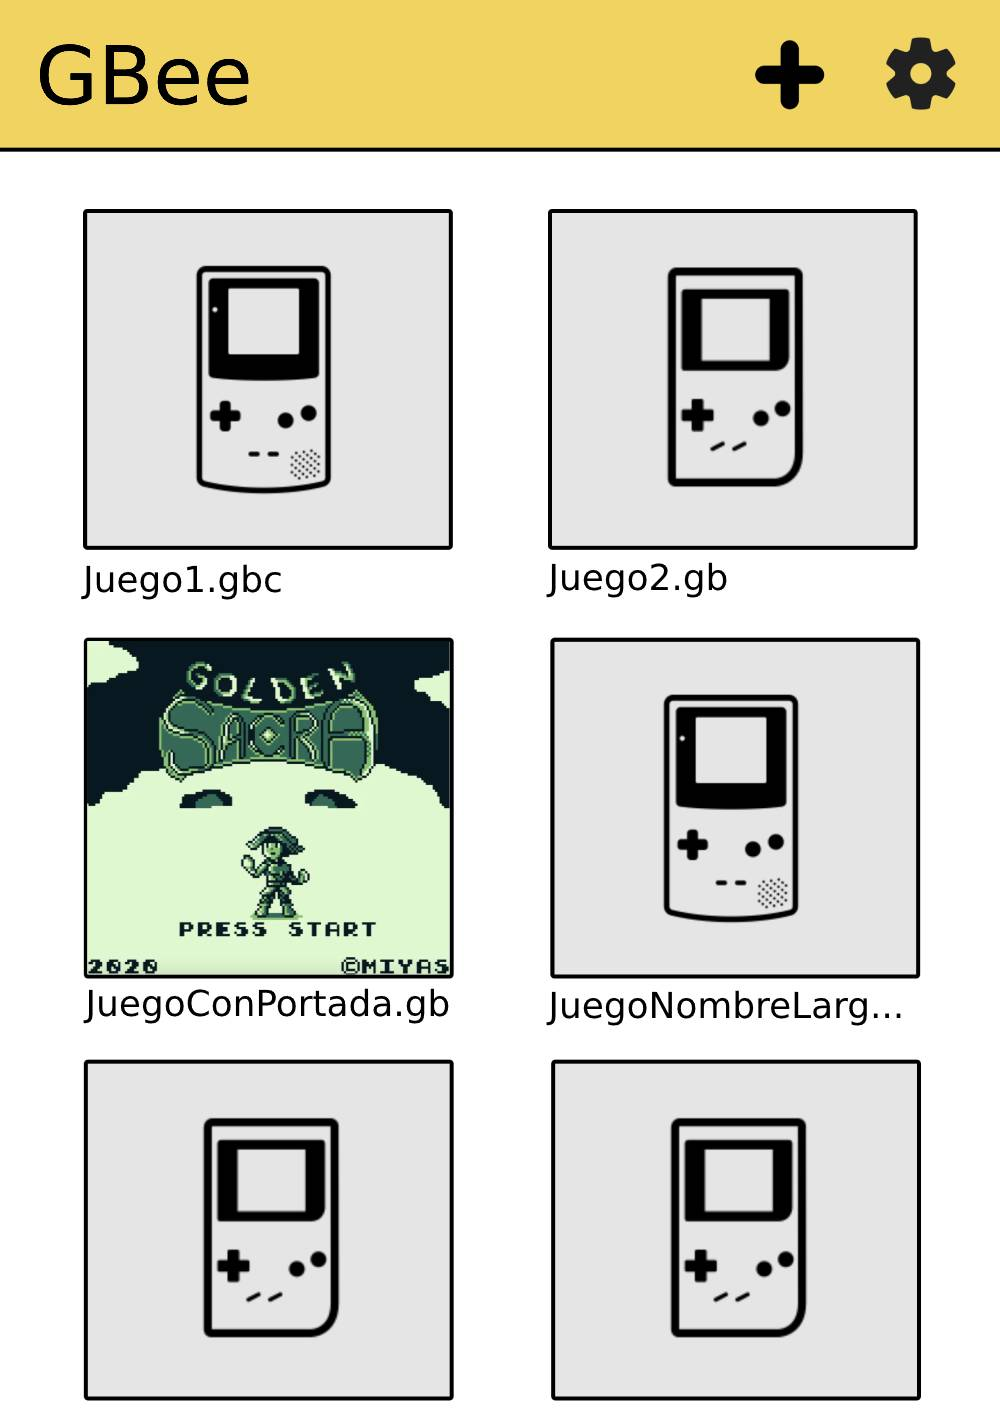
\includegraphics[width=0.4\textwidth]{include/images/mockup_menu.jpg}
    \caption{Menú de inicio.}
    \label{figure:mockupmenu}
\end{figure}

En cuanto a la pantalla de juego, se busca crear un diseño que evoque la estética de la consola original. Se incluirá un botón que brindará acceso a los ajustes del juego, el cual se ubicará, de manera provisional, en la parte superior izquierda de la pantalla. El layout será minimalista, permitiendo a los usuarios ajustar el tamaño, color y disposición de los botones según sus preferencias. La imagen de fondo tendrá un color amarillo por defecto, pero los usuarios también podrán personalizarla a su gusto. Además, se ofrecerá la opción de subir imágenes propias para reemplazar los botones o el fondo, lo que facilitará una experiencia de juego más personalizada y adaptada a los gustos individuales.
\\\\
Aunque no se representa en los mockups, se planea implementar un shader Dot-Matrix, similar al utilizado en GBCC. Esta función podrá desactivarse desde los ajustes generales de la aplicación.

\begin{figure}[h]
    \centering
    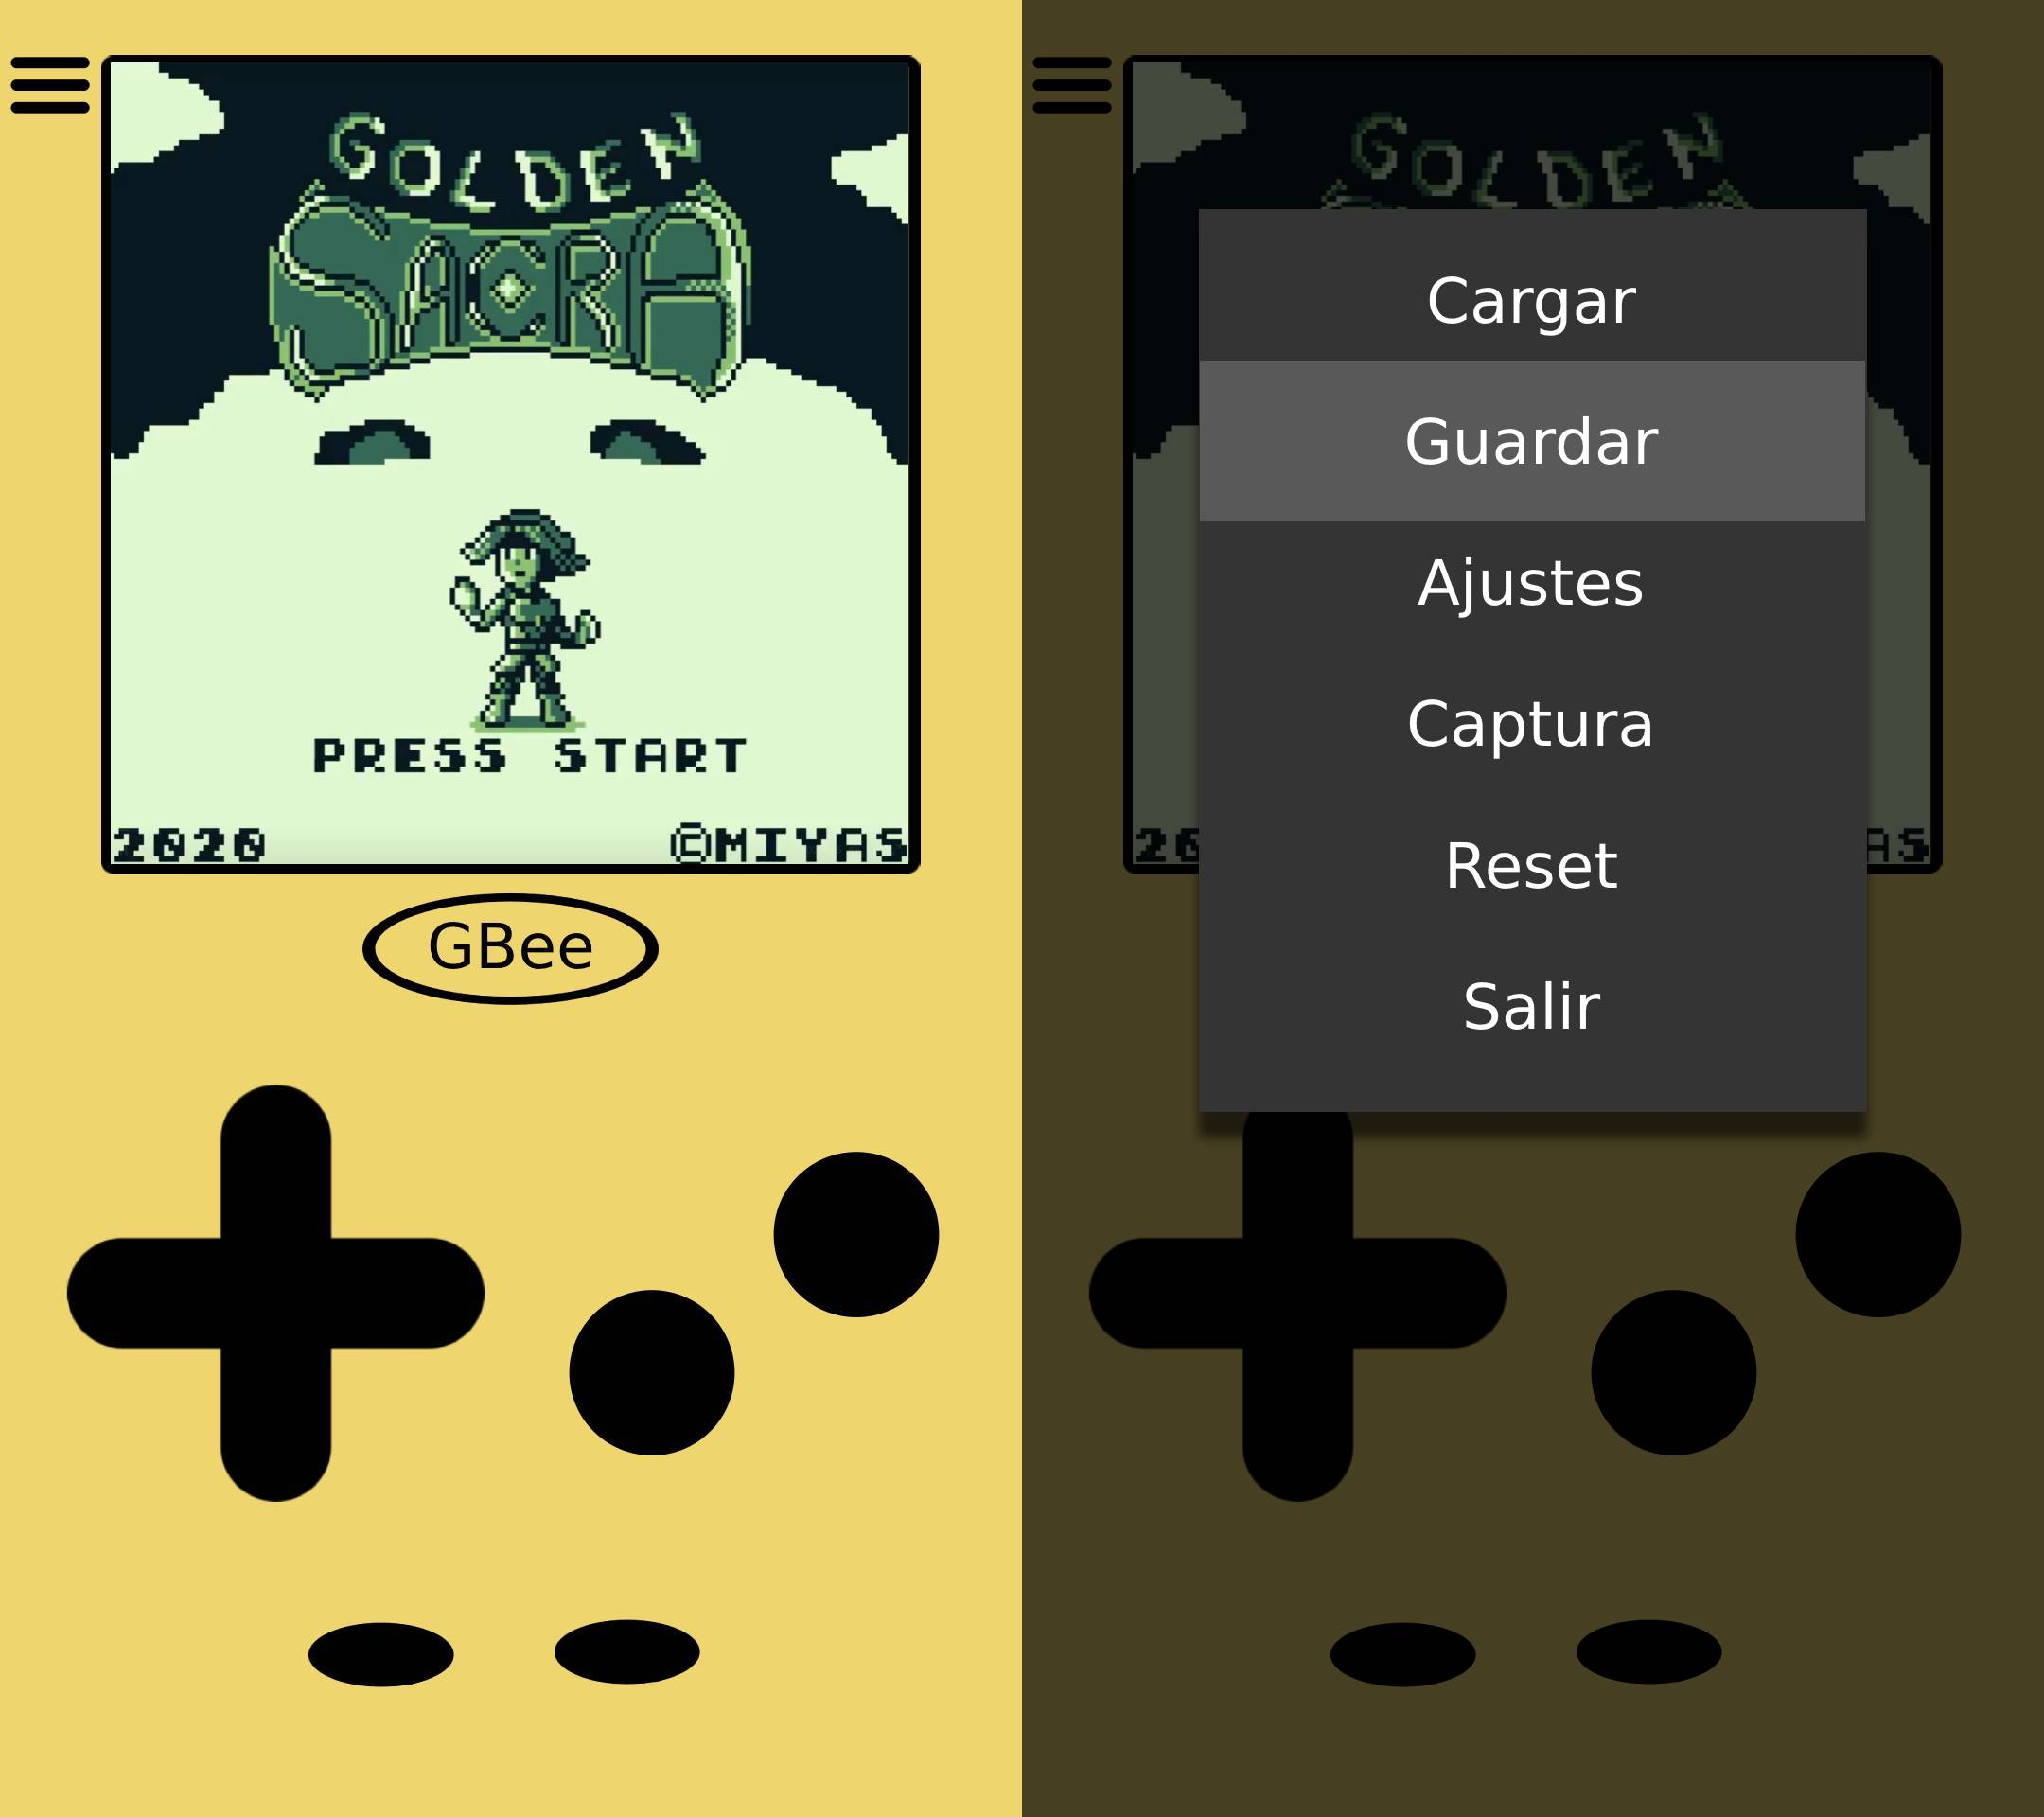
\includegraphics[width=0.6\textwidth]{include/images/mockgame.jpg}
    \caption{Pantalla de juego.}
    \label{figure:mockupgame}
\end{figure}

\cleardoublepage
\chapter{Desarrollo}
\label{develop}

El desarrollo del emulador se estructura en diversas fases que abordan los principales componentes de la consola, comenzando por la CPU, continuando con la gestión de gráficos (GPU/PPU) y memoria (RAM/ROM), y concluyendo con la implementación de las interfaces de entrada y salida (I/O). Cada uno de estos módulos es fundamental para asegurar una emulación fiel al hardware original, por lo que se prestará especial atención a la precisión y al rendimiento.
\\\\
La primera fase se centrará en la implementación de la CPU, que es responsable de ejecutar las instrucciones del juego. Cada paso del desarrollo irá acompañado de pruebas y validaciones para garantizar que el emulador reproduzca el comportamiento de la consola original de manera eficiente. Esto último se conseguirá mediante la implementación de pruebas unitarias que verifiquen el correcto comportamiento de los opcodes.

\section{Módulos / Estructura del Proyecto}

El emulador que se va a implementar constará de distintos módulos, cada uno con una función específica y clara, lo que facilitará tanto su comprensión como el desarrollo de cada uno de los aspectos del emulador. A continuación, se describen brevemente los módulos principales del proyecto:

\begin{itemize} 
    \item \textbf{Emulator}: Este módulo centraliza la gestión de los otros componentes, coordinando su interacción y asegurando que el ciclo de emulación se ejecute correctamente. Controla el flujo general del programa.
    \item \textbf{CPU}: Responsable de la ejecución de las instrucciones. Se encarga de la implementación del conjunto de instrucciones de la Game Boy y la simulación de los registros, el Program Counter (PC), el Stack Pointer (SP) y las operaciones con la ALU.
    \item \textbf{Memory}: Gestiona el acceso a la memoria principal del sistema. Proporciona una interfaz para leer y escribir datos en las distintas áreas de la memoria del emulador, incluyendo ROM, RAM y áreas de E/S.
    \item \textbf{ROM}: Módulo encargado de cargar y gestionar la memoria ROM, que contiene el código del juego o programa a emular. Lee los datos directamente desde el archivo del juego y los pone a disposición del emulador.
    \item \textbf{RAM}: Controla la memoria de acceso aleatorio del sistema, donde se almacenan temporalmente datos durante la ejecución del programa. Es volátil y se borra cada vez que se reinicia el sistema.
    \item \textbf{PPU (Pixel Processing Unit)}: Se encarga de la representación gráfica. Simula la unidad de procesamiento de píxeles de la consola, manejando la creación y renderización de sprites y fondos en pantalla.
    \item \textbf{Timer}: Simula los temporizadores de la consola, necesarios para sincronizar eventos y gestionar interrupciones relacionadas con el tiempo, como el reloj del sistema y los temporizadores de la CPU.
    \item \textbf{Interrupt}: Maneja las interrupciones generadas por los eventos del sistema, como teclas presionadas, cambios en el PPU o eventos de temporización. Se encarga de priorizarlas y derivarlas a las funciones correspondientes.
    \item \textbf{IO (Input/Output)}: Administra las interacciones de entrada y salida, como las pulsaciones de los botones del usuario y la comunicación con dispositivos externos.
    \item \textbf{DMA}: Permite la transferencia de datos entre la memoria de vídeo y la memoria principal sin la intervención del CPU. Facilita la copia eficiente de gráficos y sprites, optimizando el rendimiento al liberar al CPU para otras tareas durante las transferencias de datos.
    \item \textbf{FifoFetcher}: Gestiona la recuperación de datos de píxeles de la memoria de video, utilizando una estructura FIFO para almacenar temporalmente la información de tiles y atributos. Su función principal es asegurar una carga eficiente de píxeles para la representación gráfica en pantalla.
    \item \textbf{Audio}: Genera y manipula sonidos en la Game Boy, gestionando canales de audio como ondas de pulso y ruido. Controla la frecuencia, duración y mezcla de los sonidos.
\end{itemize}

\section{CPU}

El desarrollo comienza con la implementación de la Unidad Central de Procesamiento. Debido a su papel fundamental en la correcta reproducción del funcionamiento del sistema, esta etapa se centra en implementar todas las instrucciones para asegurar que el emulador pueda procesar cada byte de información con precisión.

\subsection{Registros}
Para definirlos en nuestro programa, utilizaremos el tipo Byte o UByte de Kotlin. En mi caso por desconocimiento del segundo tipo, comencé a programarlo con Byte. La diferencia entre ambos es que Byte utiliza el rango de [-128:128] y UByte el de [0:255] (igual que la GB). Podemos hacer uso de cualquiera de los dos mientras tengamos en mente que, si el primero lo convertimos a Integer, será un valor distinto al original. En cuanto a PC y SP, optaremos por utilizar Integers, ya que son valores de 2 bytes y siempre contienen una dirección de memoria.

\begin{lstlisting}[language=Kotlin, caption={Declaración de Registros}, label={code:kotlinregistros}]
    var A: Byte = 0
    var F: Byte = 0             // Contains the 4 flags (11110000 -> ZNHC0000)
    var B: Byte = 0
    var C: Byte = 0
    var D: Byte = 0
    var E: Byte = 0
    var H: Byte = 0
    var L: Byte = 0

    // 16 bits registers
    var SP: Int = 0xFFFE        // Stack Pointer
    var PC: Int = 0             // Program Counter
\end{lstlisting}

Para operar con ellos a nivel de byte, deberemos pasarlos a Integer, aplicarles una operación AND con el valor 0xFF (para eliminar el signo en caso de se utilice el tipo Byte originalmente), se ejecutarían las operaciones necesarias y al resultado se le aplicaría el mismo AND, para justo después volver a convertirlo a Byte:

\begin{lstlisting}[language=Kotlin, caption={Ejemplo de Opcode}, label={code:kotlinexample}]
    fun add_a_c(): Int{
        val intA = A.toInt() and 0xFF // Conversión de Byte a Integer sin signo -> A
        val intC = C.toInt() and 0xFF // Conversión de Byte a Integer sin signo -> C
        val result = intA + intC // Se suman ambos valores (ADD)
        A = (result and 0xFF).toByte() // Al resultado se le quita el signo por precaución y se convierte a Byte

        updateAddOperationFlags(intA, intC, result) // Se actualizan los Flags correspondientes

        return CYCLES_4 // Devolvemos los ciclos que la CPU debe tardar en ejecutar la instrucción
    }
\end{lstlisting}

Para la actualización de los flags, se implementarán funciones específicas que gestionarán su estado de manera adecuada. Adicionalmente, se declararán constantes que facilitarán la identificación del estado de cada flag en cualquier momento. Estas constantes corresponden a los bits asociados con un valor de 1 en formato hexadecimal (por ejemplo, 0x80 corresponde a 0b10000000).

\begin{lstlisting}[language=Kotlin, caption={Actualización de Flags}, label={code:kotlinflags}]

    // Flags --> Booleans
    const val FLAG_Z = 0x80           // Zero Flag
    const val FLAG_N = 0x40           // Subtract Flag
    const val FLAG_H = 0x20           // Half Carry Flag
    const val FLAG_C = 0x10           // Carry Flag

    [...]

    fun setFlag(flag: Int) {
        F = (F.toInt() or flag).toByte()
    }

    fun clearFlag(flag: Int) {
        F = (F.toInt() and flag.inv()).toByte()
    }

    fun updateFlag(flag: Int, condition: Boolean) {
        if (condition) {
            setFlag(flag)
        } else {
            clearFlag(flag)
        }
    }

    fun flagIsSet(flag: Int): Boolean{
        return (F.toInt() and flag) != 0
    }
\end{lstlisting}

\subsection{Opcodes}

Lo primero es identificar qué operación ejecutar dependiendo del byte que nos llegue. Podemos hacerlo de muchas maneras, en este caso lo vamos a manejar mediante un switch:

\begin{lstlisting}[language=Kotlin, caption={Identificación de Opcode}, label={code:kotlinwhen}]
    fun execute(opcode: Byte): Int {
        return when (opcode.toInt() and 0xFF) {
            0x00 -> nop()
            0x01 -> ld_bc_nn()              // LD BC, nn
            0x02 -> ld_bc_a()               // LD [BC], A
            0x03 -> inc_bc()                // INC BC
            0x04 -> inc_b()                 // INC B
            0x05 -> dec_b()                 // DEC B
            0x06 -> ld_b_n()                // LD B, n

            [...]

            0xFA -> ld_a_nn()               // LD A, [NN]
            0xFB -> ei()                    // EI
            0xFE -> cp_n()                  // CP N
            0xFF -> rst(0x0038)             // RST 38H
            else -> throw IllegalArgumentException("Instruction not supported: ${opcode.toInt() and 0xFF}")
        }
    }       
\end{lstlisting}

Para las \textbf{instrucciones extendidas}, se implementará otro switch que, de la misma forma, hará también distinción por Byte, pero al que solamente se llegará en caso de que en este primero encontremos el \textbf{Byte 0xCB}.
\\\\
En caso de que el input que nos llegue por parámetro no represente ninguna instrucción conocida, el emulador lanzará una excepción y finalizará la ejecución.
\\\\
Por cada instrucción, como ya hemos visto, deberemos tener en cuenta las características mencionadas previamente. Vamos a mostrar ejemplos de instrucciones ya implementadas por cada categoría:

\paragraph{Funciones comunes:}
Algunas funciones comunes que la gran mayoría de instrucciones van a utilizar.

\begin{lstlisting}[language=Kotlin, caption={Operaciones comunes}, label={code:kotlincommon}]
    fun fetch(): Byte {
        val byte = Memory.getByteOnAddress(PC)

        if(!cpu_halt_bug){
            PC = (PC + 1) and 0xFFFF
        }else{
            cpu_halt_bug = false
        }

        return byte
    }

    fun fetch16(): Int {
        val low = fetch().toInt() and 0xFF
        val high = fetch().toInt() and 0xFF
        return return get_16bit_address(high, low)
    }

    fun get_16bit_address(high: Byte, low: Byte): Int{
        return ((high.toInt() and 0xFF) shl 8) or (low.toInt() and 0xFF)
    }

    fun set_16bit_address_value(high: Byte, low: Byte, value: Byte){
        val address = get_16bit_address(high, low)
        Memory.writeByteOnAddress(address, value)
    }
\end{lstlisting}

La función \textit{fetch()} tiene como objetivo principal obtener el byte almacenado en la dirección de memoria señalada por el PC, e incrementarlo posteriormente (si no se produce el fallo de la CPU, que será explicado más adelante). 
\\\\
Por su parte, \textit{fetch16()} realiza dos llamadas consecutivas a \textit{fetch()} y combina los dos bytes obtenidos mediante la función \textit{get\_16bit\_address()}, que utiliza las operaciones SHL y OR. 
\\\\
Finalmente, la función \textit{set\_16bit\_address\_value()}, recibe una dirección como parámetro y delega al módulo de memoria la escritura del valor proporcionado, si es posible hacerlo.

\paragraph{Carga - LD:}\label{instrLd}

Añadimos de ejemplo cuatro funciones de las cuales podemos derivar el resto. En todos ellos se van a devolver los ciclos de reloj correspondientes.

\begin{lstlisting}[language=Kotlin, caption={Operaciones LD}, label={code:kotlinld}]
    fun ld_c_l(): Int{
        C = L
        return CYCLES_4
    }

    fun ld_c_hl(): Int{
        val hl = get_16bit_address(H, L)
        C = Memory.getByteOnAddress(hl)
        return CYCLES_8
    }

    fun ld_hl_b(): Int{
        set_16bit_address_value(H, L, B)
        return CYCLES_8
    }

    fun ld_hl_nn(): Int{
        val low = fetch().toInt() and 0xFF
        val high = fetch().toInt() and 0xFF
        H = high.toByte()
        L = low.toByte()

        return CYCLES_12
    }
\end{lstlisting}

En la primera función (LD C, L) simplemente se carga el contenido del registro L en C.
\\\\
En la siguiente (LD C, [HL]) lo que se debe hacer es obtener el byte almacenado en la dirección de memoria señalada por HL y cargarlo en C (para ello hacemos uso del módulo de memoria).
\\\\
La tercera función (LD [HL], B) es justo lo contrario a la segunda. En este caso lo que hacemos es guardar el byte del registro B en la dirección de memoria ya especificada en HL.
\\\\
Por último, en la cuarta función (LD [HL], NN), no nos viene especificado un registro, si no que debemos obtener los dos siguientes bytes del PC. Hay que recordar que los bytes se guardan en memoria en \textbf{Little Endian}, por lo que el primero que se obtiene es el Low. Asignamos al registro H el High y al registro L el Low, y al devolver los ciclos correspondientes quedaría implementada la instrucción.

\paragraph{Aritméticas y Lógicas:} En esta categoría entran todas las instrucciones de ADD, ADC, AND, SUB, SBC, DEC, INC, XOR, OR, CP, CPL, CCF, DAA y SCF. Vamos a ver algunos ejemplos de cada una de ellas:

\begin{lstlisting}[language=Kotlin, caption={Operaciones ADD y ADC}, label={code:kotlinaddc}]
    fun updateAddOperationFlags(val1: Int, val2: Int, result: Int){
        updateFlag(FLAG_Z, result == 0)
        clearFlag(FLAG_N)
        updateFlag(FLAG_H, (val1 and 0xF) + (val2 and 0xF) > 0xF)
        updateFlag(FLAG_C, result > 0xFF)
    }

    fun add_a_b(): Int{
        val intA = A.toInt() and 0xFF
        val intB = B.toInt() and 0xFF
        val result = intA + intB
        A = (result and 0xFF).toByte()

        updateAddOperationFlags(intA, intB, result)

        return CYCLES_4
    }

    fun adc_a_b(): Int{
        val carry = if (flagIsSet(FLAG_C)) 1 else 0
        val intA = A.toInt() and 0xFF
        val intB = B.toInt() and 0xFF
        val result = intA + (intB + carry)
        A = (result and 0xFF).toByte()

        updateAddOperationFlags(intA, intB + carry, result)

        return CYCLES_4
    }
\end{lstlisting}

Para la instrucción \textbf{ADD} (en este caso \textbf{ADD A, B}), la operación consiste en convertir ambos registros a enteros sin signo y sumar sus valores.
\\\\
La diferencia entre ADD y ADC reside en que en este último al resultado también se le suma el valor del carry y, por ende, se debe tener en cuenta en la actualización del flag Half-Carry.
\\\\
En los casos que impliquen el uso de direcciones de memoria (operaciones de 2 bytes), se puede emplear el código utilizado en las instrucciones de carga (LD) \ref{instrLd} como referencia.

\begin{lstlisting}[language=Kotlin, caption={Operaciones INC y DEC}, label={code:kotlinincdec}]
    fun inc_8bit_register(register: Byte): Byte{
        val toReturn = (register.toInt() + 1).toByte()
        updateFlag(FLAG_Z, toReturn.toInt() == 0x00)
        clearFlag(FLAG_N)
        updateFlag(FLAG_H, ((register.toInt() and 0xF) + 1) and 0x10 != 0x00)
        return toReturn
    }

    fun dec_8bit_register(register: Byte): Byte{
        val toReturn = (register.toInt() - 1).toByte()
        updateFlag(FLAG_Z, toReturn.toInt() == 0x00)
        setFlag(FLAG_N)
        updateFlag(FLAG_H, (register.toInt() and 0xF == 0x00))
        return toReturn
    }

    fun inc_bc(): Int{
        val oldValue = get_16bit_address(B, C)
        val newValue = (oldValue + 1) and 0xFFFF
        B = (newValue shr 8).toByte()
        C = newValue.toByte()
        return CYCLES_8
    }

    fun dec_b(): Int{
        B = dec_8bit_register(B)
        return CYCLES_4
    }

    fun inc_b(): Int{
        B = inc_8bit_register(B)
        return CYCLES_4
    }
\end{lstlisting}

Las instrucciones de INC y DEC son muy similares. INC suma 1 al valor y afecta los flags del procesador: el Zero (Z) se activa si el resultado es 0, el Half-carry (H) se activa si hay un acarreo entre los bits 3 y 4, y el Subtract (N) siempre se borra. Por su parte, DEC resta 1 al valor y afecta los mismos flags, pero siempre activa el Subtract (N) ya que es una operación de sustracción. Ambos opcodes no afectan el Carry flag (C) y se utilizan tanto para registros de 8 bits como para posiciones de memoria.

\begin{lstlisting}[language=Kotlin, caption={Operación XOR}, label={code:kotlinxor}]
    fun xor_b(): Int{
        A = (((A.toInt() and 0xFF) xor (register.toInt()) and 0xFF)).toByte()

        updateFlag(FLAG_Z, (A.toInt() and 0xFF) == 0)
        clearFlag(FLAG_N)
        clearFlag(FLAG_H)
        clearFlag(FLAG_C)
        
        return CYCLES_4
    }
\end{lstlisting}

La operación XOR se realizan siempre al registro A, utilizando su valor y el del registro indicado por el opcode (en este caso B). Tras la operación, verifica si el resultado es cero para activar el flag Z, y limpia los flags N, H y C, ya que no son relevantes.
\\\\
Las operaciones OR son idénticas en Kotlin, simplemente deberemos cambiar el operando 'xor' por 'or'.

\paragraph{Control de flujo:} Las instrucciones de control de flujo, como CALL, JP y RETI, permiten modificar la secuencia de ejecución del programa. Estas instrucciones desvían el flujo normal de instrucciones al saltar a direcciones específicas de memoria o retornar desde subrutinas o interrupciones. Tenemos instrucciones como CALL, JP o JR que son utilizadas para saltar a una nueva dirección, con CALL almacenando la dirección de retorno en la pila para permitir volver al punto de origen.
\\\\
Vamos a analizarlas de una en una:
\begin{lstlisting}[language=Kotlin, caption={Operación CALL}, label={code:kotlincall}]
    fun call_nz_nn(): Int{
        val address = fetch16()

        if (!flagIsSet(FLAG_Z)) {
            SP = (SP - 1) and 0xFFFF
            Memory.writeByteOnAddress(SP, (PC ushr 8).toByte()) // Alto
            SP = (SP - 1) and 0xFFFF
            Memory.writeByteOnAddress(SP, (PC and 0xFF).toByte()) // Bajo
    
            PC = address
            return CYCLES_24
        }

        return CYCLES_12
    }
\end{lstlisting}

La instrucción \textbf{CALL} salta a una subrutina especificada, guardando la dirección de retorno en la pila. El PC se actualiza con la dirección de destino, y tras ejecutar la subrutina, el programa puede volver al punto original usando la instrucción RET, restaurando la dirección desde la pila. Esta último instrucción no se implementa en el propio CALL, si no que debe ser gestionada a posterior por parte del desarrollador, utilizando el valor previo del PC (guardado en el SP antes de su actualización).
\\\\
Además, en el ejemplo expuesto, se nos indica que el CALL solamente se debe ejecutar si el Flag Z no está activo. En caso contrario, lo único que haría son 2 \textit{fetch()} seguidos y se hace uso de menos ciclos de reloj.

\begin{lstlisting}[language=Kotlin, caption={Operaciones JR y JP}, label={code:kotlinjpjr}]
    fun jr_n(): Int{
        val offset = fetch()
        PC += offset.toInt()
        return CYCLES_12
    }

    fun jp_nn(): Int{
        val address = fetch16()
        PC = address
        return CYCLES_16
    }
\end{lstlisting}

Las instrucciones \textbf{JR} y \textbf{JP} son similares a CALL, pero no almacenan el valor actual del PC en el stack. 
\\\\
La instrucción JP salta directamente a una dirección de memoria especificada, actualizando el PC, lo que permite saltos largos a cualquier posición en la memoria. 
\\\\
JR, en cambio, realiza un salto relativo, ajustando el PC en función de un desplazamiento positivo o negativo, permitiendo saltos más cortos dentro de un rango cercano. Dado que los \textbf{saltos relativos} pueden cubrir un \textbf{máximo de 0xFF bytes} hacia arriba o abajo, JR consume menos ciclos de reloj.

\begin{lstlisting}[language=Kotlin, caption={Operaciones RET y RETI}, label={code:kotlinreti}]
    fun executeRetOperation(){
        val low = Memory.getByteOnAddress(SP).toInt() and 0xFF
        SP = (SP + 1) and 0xFFFF
        val high = Memory.getByteOnAddress(SP).toInt() and 0xFF
        SP = (SP + 1) and 0xFFFF

        PC = (high shl 8) or low
    }

    fun ret(): Int{
        executeRetOperation()
        return CYCLES_16
    }

    fun reti(): Int{
        executeRetOperation()
        Interrupt.enableInterrupts(true)
        return CYCLES_16
    }
\end{lstlisting}

Las instrucciones \textbf{RET} y \textbf{RETI} se utilizan para retornar de una subrutina, recuperando la dirección de retorno almacenada en el stack. RET restaura el valor del registro PC desde el stack, permitiendo así continuar la ejecución desde donde se dejó al llamar a la subrutina. En contraste, RETI realiza la misma operación, pero se utiliza específicamente para el retorno de una interrupción, asegurando que se manejen correctamente las interrupciones pendientes antes de restaurar el flujo de ejecución.

\begin{lstlisting}[language=Kotlin, caption={Operación CP}, label={code:kotlincp}]
    fun cp_b(): Int{
        val intA = A.toInt() and 0xFF
        val intRegister = B.toInt() and 0xFF

        val result = (intA - intRegister) and 0xFF

        updateFlag(FLAG_Z, result == 0)
        setFlag(FLAG_N)
        updateFlag(FLAG_H, (intA and 0xF) < (intRegister and 0xF))
        updateFlag(FLAG_C, intA < intRegister)
        
        return CYCLES_4
    }
\end{lstlisting}

La función CP B (Compare B) se encarga de comparar el valor del registro A con el valor del registro B, estableciendo los flags correspondientes según el resultado de la comparación. Primero, convierte los registros A y B a enteros de 8 bits, luego calcula el resultado de la resta entre A y B, enmascarando el resultado para asegurarse de que se mantenga dentro del rango de 8 bits. A continuación, actualiza el flag Z si el resultado es igual a cero, establece el flag N para indicar que se realizó una comparación, y determina el estado del flag H al verificar si el nibble menos significativo de A es menor que el de B. Por último, establece el flag C si el valor de A es menor que el de B.

\begin{lstlisting}[language=Kotlin, caption={Operación CPL}, label={code:kotlincpl}]
    fun cpl(): Int{

        A = (A.toInt() xor 0xFF).toByte()

        setFlag(FLAG_N)
        setFlag(FLAG_H)

        return CYCLES_4
    }
\end{lstlisting}

La función CPL (Complementary) se encarga de complementar el valor del registro A, invirtiendo todos sus bits mediante una operación XOR con 0xFF. Esto transforma todos los bits de A en sus opuestos, cambiando ceros por unos y viceversa. Después de realizar la operación, la función establece el flag N para indicar que se ha realizado una operación que afecta al signo del número, y también establece el flag H para indicar que puede haber un acarreo en la operación.

\begin{lstlisting}[language=Kotlin, caption={Operación CCF}, label={code:kotlinccf}]
    fun ccf(): Int{

        val newCarry = ((F.toInt() and 0xFF) and FLAG_C) == 0
        updateFlag(FLAG_C, newCarry)
        setFlag(FLAG_N)
        setFlag(FLAG_H)

        return CYCLES_4
    }
\end{lstlisting}

La función CCF (Complement Carry Flag) se encarga de complementar el valor del flag C. Primero, verifica si el flag de acarreo está actualmente activado; si no lo está, lo activa, y si lo está, lo desactiva, utilizando el operador lógico AND para determinar su estado anterior. Además, establece los flags H y N como activos.

\begin{lstlisting}[language=Kotlin, caption={Operación DAA}, label={code:kotlindaa}]
    fun daa(): Int{

        var result = A.toInt() and 0xFF

        if (!flagIsSet(FLAG_N)) { // Addition

            if ((result and 0x0F) > 9 || flagIsSet(FLAG_H)) // Lower nibble
                result += 0x06

            if ((result and 0xF0) > 0x90 || flagIsSet(FLAG_C)) // Higher nibble
                result += 0x60

        }else{ // Substraction
            if (flagIsSet(FLAG_H)) // Lower nibble
                result -= 0x06

            if (flagIsSet(FLAG_C)) // Higher nibble
                result -= 0x60
        }

        updateFlag(FLAG_Z, (result and 0xFF) == 0x00)
        clearFlag(FLAG_H)
        updateFlag(FLAG_C, result > 0xFF)

        result = result and 0xFF
        A = result.toByte()

        return CYCLES_4
    }
\end{lstlisting}

La función DAA (Decimal Adjust for Addition) es una implementación que ajusta el valor del registro A para operaciones aritméticas en formato decimal después de una suma o resta. El método primero convierte el valor de A a un entero de 8 bits, luego verifica si la operación anterior fue una suma o una resta basándose en el estado del flag N.

\begin{lstlisting}[language=Kotlin, caption={Operación SCF}, label={code:kotlinscf}]
    fun scf(): Int{

        clearFlag(FLAG_N)
        clearFlag(FLAG_H)
        setFlag(FLAG_C)

        return CYCLES_4
    }
\end{lstlisting}

La función SCF (Set Carry Flag) establece el flag C a 1 y borra los flags N y H, lo que indica que el próximo cálculo tendrá en cuenta que se ha producido un acarreo.

\paragraph{Rotación y desplazamiento:} En esta categoría tenemos las instrucciones de RL, RR, RLC, RRC, SLA, SRA, SWAP y SRL. Vamos a ver algunos ejemplos de cada una de ellas:

\begin{lstlisting}[language=Kotlin, caption={Operaciones RL y RR}, label={code:kotlinrlrr}]
    fun rl_b(): Int{
        val bByte = B.toInt() and 0xFF
        val oldCarry = if (flagIsSet(FLAG_C)) 1 else 0
        val newCarry = (bByte ushr 7) and 0x1

        B = ((bByte shl 1) or oldCarry).toByte()

        updateFlag(FLAG_Z, B == 0.toByte())
        clearFlag(FLAG_N)
        clearFlag(FLAG_H)
        updateFlag(FLAG_C, newCarry == 1)

        return CYCLES_8
    }
    
    fun rr_b(): Int{
        val bByte = B.toInt() and 0xFF
        val oldCarry = if (flagIsSet(FLAG_C)) 1 else 0
        val newCarry = (bByte ushr 7) and 0x1

        B = ((bByte shr 1) or (oldCarry shl 7)).toByte()

        updateFlag(FLAG_Z, B == 0.toByte())
        clearFlag(FLAG_N)
        clearFlag(FLAG_H)
        updateFlag(FLAG_C, newCarry == 1)

        return CYCLES_8
    }
\end{lstlisting}

Las funciones RL B y RR B realizan rotaciones de bits en el registro B, pero difieren en la dirección y el manejo del carry. La función RL rota los bits hacia la izquierda; el MSB se desplaza a la izquierda y se introduce en el LSB, utilizando el valor del carry anterior para completar la rotación. En cambio, RR rota los bits hacia la derecha; el LSB se mueve al carry y el carry anterior se coloca en el MSB. Ambas funciones actualizan los indicadores de estado, como el flag Z si el resultado es cero, y el flag C según el bit que se desplaza.

\begin{lstlisting}[language=Kotlin, caption={Operaciones RLC y RRC}, label={code:kotlinrlcrrc}]
    fun rlc_b(): Int{
        val bByte = B.toInt() and 0xFF
        val carry = (bByte ushr 7) and 0x1
        B = ((bByte shl 1) or carry).toByte()

        updateFlag(FLAG_Z, B == 0.toByte())
        clearFlag(FLAG_N)
        clearFlag(FLAG_H)
        updateFlag(FLAG_C, carry == 1)

        return CYCLES_8
    }

    fun rrc_b(): Int{
        val bByte = B.toInt() and 0xFF
        val carry = bByte and 0x1
        B = ((bByte shr 1) or (carry shl 7)).toByte()

        updateFlag(FLAG_Z, B == 0.toByte())
        clearFlag(FLAG_N)
        clearFlag(FLAG_H)
        updateFlag(FLAG_C, carry == 1)

        return CYCLES_8
    }
\end{lstlisting}

La función RLC B realiza una rotación a la izquierda del registro B, desplazando el MSB hacia el LSB y estableciendo el nuevo valor del MSB en el carry. Actualiza todos los flags en función del resultado. En contraste, la función RRC B efectúa una rotación a la derecha, desplazando el LSB hacia el MSB y estableciendo su nuevo valor en el carry.

\begin{lstlisting}[language=Kotlin, caption={Operaciones SLA, SRA y SRL}, label={code:kotlinslasrasrl}]
    fun sla_b(): Int{
        val bByte = B.toInt() and 0xFF
        val newCarry = (bByte ushr 7) and 0x1
        B = ((bByte shl 1) and 0xFE).toByte()

        updateFlag(FLAG_Z, B == 0.toByte())
        clearFlag(FLAG_N)
        clearFlag(FLAG_H)
        updateFlag(FLAG_C, newCarry == 1)
        
        return CYCLES_8
    }

    fun sra_b(): Int{
        val bByte = B.toInt() and 0xFF
        val oldBit7 = bByte and 0x80
        val newCarry = bByte and 0x1

        B = ((bByte shr 1) or oldBit7).toByte()

        updateFlag(FLAG_Z, B == 0.toByte())
        clearFlag(FLAG_N)
        clearFlag(FLAG_H)
        updateFlag(FLAG_C, newCarry == 1)

        return CYCLES_8
    }

    fun srl_b(): Int{
        val bByte = B.toInt() and 0xFF
        val newCarry = bByte and 0x1
        B = ((bByte shr 1) and 0x7F).toByte()

        updateFlag(FLAG_Z, B == 0.toByte())
        clearFlag(FLAG_N)
        clearFlag(FLAG_H)
        updateFlag(FLAG_C, newCarry == 1)

        return CYCLES_8
    }
\end{lstlisting}

La función SLA B realiza un desplazamiento lógico a la izquierda del registro B, moviendo todos los bits una posición a la izquierda y estableciendo el LSB en 0, mientras que el nuevo carry se toma del antiguo MSB. En contraste, SRA B realiza un desplazamiento aritmético a la derecha, manteniendo el bit más significativo y moviendo el resto de los bits hacia la derecha, con el nuevo carry tomado del antiguo LSB. Por otro lado, SRL B también realiza un desplazamiento lógico a la derecha, pero establece el MSB en 0 y mueve los bits a la derecha, con el nuevo carry tomado del antiguo LSB.

\begin{lstlisting}[language=Kotlin, caption={Operación SWAP}, label={code:kotlinswap}]
    fun swap_b(): Int{
        val bByte = B.toInt() and 0xFF
        val low = (bByte and 0x0F) shl 4
        val high = (bByte and 0xF0) shr 4
        B = (low or high).toByte()

        updateFlag(FLAG_Z, B == 0.toByte())
        clearFlag(FLAG_N)
        clearFlag(FLAG_H)
        clearFlag(FLAG_C)

        return CYCLES_8
    }
\end{lstlisting}

La función SWAP B intercambia los nibbles (4 bits) del registro B, moviendo los 4 bits menos significativos a la posición de los 4 bits más significativos y viceversa. Actualiza el flag Z si el nuevo valor es cero, y limpia los flags N, H y C.

\paragraph{Manipulación de bits:} Encontramos las instrucciones BIT, RES y SET.

\begin{lstlisting}[language=Kotlin, caption={Operación BIT}, label={code:kotlinbit}]
    fun updateBitOperationFlags(result: Boolean){
        updateFlag(FLAG_Z, result)
        clearFlag(FLAG_N)
        setFlag(FLAG_H)
    }

    fun bit_operation(register: Int, bitNumber: Int): Int{

        require(bitNumber in 0..7) { "Bit must be between 0 and 7" }
        require(register in 1..8) { "Register must be between 1 and 8" }

        var bitZero = false
        var cyclesToReturn = CYCLES_8
        val bit = 0x1 shl bitNumber

        when (register) {
            1 -> bitZero = ((B.toInt() and 0xFF) and bit) == 0
            2 -> bitZero = ((C.toInt() and 0xFF) and bit) == 0
            3 -> bitZero = ((D.toInt() and 0xFF) and bit) == 0
            4 -> bitZero = ((E.toInt() and 0xFF) and bit) == 0
            5 -> bitZero = ((H.toInt() and 0xFF) and bit) == 0
            6 -> bitZero = ((L.toInt() and 0xFF) and bit) == 0
            7 -> {
                val address = get_16bit_address(H, L)
                bitZero = ((Memory.getByteOnAddress(address).toInt() and 0xFF) and bit) == 0
                cyclesToReturn = CYCLES_16
            }
            8 -> bitZero = ((A.toInt() and 0xFF) and bit) == 0
        }

        updateBitOperationFlags(bitZero)
        return cyclesToReturn
    }
\end{lstlisting}

La operación BIT verifica el estado de un bit específico (de 0 a 7) en un registro determinado (de 1 a 8). Utiliza condiciones para identificar qué registro se está evaluando y calcula si el bit indicado está apagado (0) o encendido (1). Si el registro es 7, que representa una dirección de memoria, obtiene el byte correspondiente desde esa dirección, y el tiempo de ciclo se ajusta a 16. Posteriormente, actualiza el flag Z, limpia el flag N y establece el flag H. Al final, devuelve el tiempo de ciclo correspondiente, que es 8 para los registros de 1 a 6 y el 8, y 16 para el registro 7.

\begin{lstlisting}[language=Kotlin, caption={Operación RES}, label={code:kotlinres}]
    fun res_operation(register: Int, bitNumber: Int): Int{

        require(bitNumber in 0..7) { "Bit must be between 0 and 7" }
        require(register in 1..8) { "Register must be between 1 and 8" }

        var cyclesToReturn = CYCLES_8
        val bit = (0x1 shl bitNumber).inv()

        when (register) {
            1 -> B = ((B.toInt() and 0xFF) and bit).toByte()
            2 -> C = ((C.toInt() and 0xFF) and bit).toByte()
            3 -> D = ((D.toInt() and 0xFF) and bit).toByte()
            4 -> E = ((E.toInt() and 0xFF) and bit).toByte()
            5 -> H = ((H.toInt() and 0xFF) and bit).toByte()
            6 -> L = ((L.toInt() and 0xFF) and bit).toByte()
            7 -> {
                val address = get_16bit_address(H, L)
                val result = ((Memory.getByteOnAddress(address).toInt() and 0xFF) and bit).toByte()
                Memory.writeByteOnAddress(address, result)
                cyclesToReturn = CYCLES_16
            }
            8 -> A = ((A.toInt() and 0xFF) and bit).toByte()
        }

        return cyclesToReturn
    }
\end{lstlisting}

La operación RES se encarga de reiniciar (poner a 0) un bit específico (de 0 a 7) en un registro determinado (de 1 a 8). Utiliza condiciones para determinar cuál registro se está manipulando y genera una máscara de bit que apaga el bit correspondiente. Si el registro es 7, la función obtiene la dirección de memoria desde los registros H y L, lee el byte almacenado en esa dirección, reinicia el bit correspondiente y escribe el nuevo valor de vuelta en memoria. El tiempo de ciclo se gestiona de la misma manera que en la operación BIT.

\begin{lstlisting}[language=Kotlin, caption={Operación SET}, label={code:kotlinset}]
    fun set_operation(register: Int, bitNumber: Int): Int{

        require(bitNumber in 0..7) { "Bit must be between 0 and 7" }
        require(register in 1..8) { "Register must be between 1 and 8" }

        var cyclesToReturn = CYCLES_8
        val bit = 0x1 shl bitNumber

        when (register) {
            1 -> B = ((B.toInt() and 0xFF) or bit).toByte()
            2 -> C = ((C.toInt() and 0xFF) or bit).toByte()
            3 -> D = ((D.toInt() and 0xFF) or bit).toByte()
            4 -> E = ((E.toInt() and 0xFF) or bit).toByte()
            5 -> H = ((H.toInt() and 0xFF) or bit).toByte()
            6 -> L = ((L.toInt() and 0xFF) or bit).toByte()
            7 -> {
                val address = get_16bit_address(H, L)
                val result = ((Memory.getByteOnAddress(address).toInt() and 0xFF) or bit).toByte()
                Memory.writeByteOnAddress(address, result)
                cyclesToReturn = CYCLES_16
            }
            8 -> A = ((A.toInt() and 0xFF) or bit).toByte()
        }

        return cyclesToReturn
    }
\end{lstlisting}

La operación SET se encarga de establecer (poner a 1) un bit específico (de 0 a 7) en un registro determinado (de 1 a 8). Utiliza condiciones para identificar qué registro se está manipulando y genera una máscara de bit que activa el bit correspondiente. Si el registro es 7, la función obtiene la dirección de memoria a partir de los registros H y L, lee el byte almacenado en esa dirección, activa el bit correspondiente y escribe el nuevo valor de vuelta en la memoria. El tiempo de ciclo se gestiona de la misma manera que en la operación BIT.

\paragraph{Especiales de sistema:} Encontramos las instrucciones NOP, DI y EI:

\begin{lstlisting}[language=Kotlin, caption={Operación NOP}, label={code:kotlinnop}]
    fun nop(): Int{
        return CYCLES_4
    }
\end{lstlisting}

La operación NOP (No Operation) realiza una operación que no tiene efecto en el estado del procesador; es decir, no cambia los registros, la memoria o los flags. Su principal función es ocupar espacio en el ciclo de ejecución, permitiendo la sincronización en la ejecución de instrucciones o como un marcador para pausas en el código. A la hora de implementarlo, simplemente devolvemos los ciclos correspondientes.

\begin{lstlisting}[language=Kotlin, caption={Operaciones DI, EI}, label={code:kotlindiei}]
    private var pendingEI = false

    [...]

    fun ei(): Int{
        pendingEI = true
        return CYCLES_4
    }

    fun di(): Int{
        Interrupt.enableInterrupts(false)
        return CYCLES_4
    }
\end{lstlisting}

El opcode EI habilita las interrupciones en el procesador (se detallará más adelante). Es importante destacar que las interrupciones no se activan de manera inmediata; en su lugar, deben esperar hasta el siguiente ciclo de la CPU para entrar en efecto. Por esta razón, se utiliza una variable para almacenar el estado de las interrupciones.
\\\\
Por otro lado, DI deshabilita las interrupciones en el procesador, bloqueando la capacidad del sistema para responder a señales externas hasta que se vuelvan a habilitar mediante un EI. En este caso, los cambios si que tienen efecto inmediato.

\paragraph{Con pila:} Encontramos las instrucciones PUSH y POP:

\begin{lstlisting}[language=Kotlin, caption={Operaciones PUSH, POP}, label={code:kotlinpushpop}]
    fun push_bc(): Int{
        SP = (SP - 1) and 0xFFFF
        Memory.writeByteOnAddress(SP, B) // high
        SP = (SP - 1) and 0xFFFF
        Memory.writeByteOnAddress(SP, C) // low

        return CYCLES_16
    }

    fun pop_bc(): Int{

        C = Memory.getByteOnAddress(SP)
        SP = (SP + 1) and 0xFFFF
        B = Memory.getByteOnAddress(SP)
        SP = (SP + 1) and 0xFFFF

        return CYCLES_12
    }
\end{lstlisting}

La función PUSH BC almacena los valores de los registros B y C en la pila. Primero, decrece el puntero de la pila (SP) en 1 y escribe el contenido de B en la dirección de memoria apuntada, luego vuelve a decrecer la pila y escribe el contenido de C. Esta operación asegura que el registro C se almacene en la parte baja de la pila y B en la parte alta.

Por otro lado, la función POP BC recupera los valores de los registros B y C desde la pila. Comienza leyendo el byte almacenado en la dirección de memoria apuntada por SP y lo asigna al registro C, luego incrementa la pila para apuntar al siguiente byte. A continuación, lee el byte en la nueva dirección y lo asigna al registro B, y nuevamente incrementa SP.

\begin{lstlisting}[language=Kotlin, caption={Operaciones I/O}, label={code:kotlinio}]
    fun ldh_n_a(): Int{

        val byte = fetch().toInt() and 0xFF
        val address = (0xFF00 + byte) and 0xFFFF
        Memory.writeByteOnAddress(address, A)

        return CYCLES_12
    }

    fun ld_cn_a(): Int{
        val address = (0xFF00 + (C.toInt() and 0xFF)) and 0xFFFF
        Memory.writeByteOnAddress(address, A)
        return CYCLES_8
    }
\end{lstlisting}

La función LDH N, A carga el valor del registro A en una dirección de memoria específica determinada por un byte que se obtiene mediante la función fetch(). Este byte se suma a la dirección base 0xFF00 (dirección en la que empiezan los registros de I/O) para formar la dirección final donde se almacenará el valor de A.
\\\\
Por otro lado, la función LD CN, A almacena el valor del registro A en una dirección de memoria también basada en el registro C. Aquí, se suma el valor de C a la dirección base 0xFF00 para calcular la dirección final, donde se escribirá el valor de A.
\\\\
Ambas funciones son importantes para la manipulación de datos en la memoria del sistema.

\section{Memory}
El módulo de memoria actúa como un bus de datos que redirecciona las operaciones de lectura y escritura hacia otros módulos del emulador, como la CPU, la ROM y otros componentes. Además de su función de interconexión, este módulo contiene toda la memoria virtual principal de nuestro emulador, que abarca los 64 KB de espacio de memoria direccionable. Esto incluye tanto la memoria de trabajo, como la RAM, como la memoria de mapeo de la ROM, que se utiliza para cargar los juegos.
\\\\
Comenzaremos la implementación declarando algunas constantes y la variable correspondiente que reservará esos 64KB de memoria:

\begin{lstlisting}[language=Kotlin, caption={Declaraciones iniciales de Memoria}, label={code:kotlinmem}]
    const val ROM_START             = 0x0000
    const val ROM_SW_START          = 0x4000
    const val ROM_END               = 0x7FFF
    const val BOOT_END              = 0x00FF
    const val VRAM_START            = 0x8000
    const val VRAM_END              = 0x9FFF
    const val EXTERNAL_RAM_START    = 0xA000
    const val WRAM_START            = 0xC000
    const val FIXED_WRAM_END        = 0xCFFF
    const val SWITCHABLE_WRAM_START = 0xD000
    const val ECHO_RAM_START        = 0xE000
    const val OAM_START             = 0xFE00
    const val RESERVED_MEM_START    = 0xFEA0
    const val IO_START              = 0xFF00
    const val HRAM_START            = 0xFF80
    const val HRAM_END              = 0xFFFE
    
    const val MEMORY_SIZE   = 0x10000   // 64 KB
    const val BOOT_SIZE     = 0xFF

    [...]

    private val memory = ByteArray(MEMORY_SIZE)
\end{lstlisting}

\subsection{Lectura / Escritura}

Al realizar operaciones de lectura y escritura, no podemos simplemente asignar un valor directamente a la dirección proporcionada como parámetro. Existen áreas de memoria donde los desarrolladores tienen restricciones para escribir y otras a las que no se puede acceder en determinados momentos de la ejecución. Por esta razón, delegaremos las funciones de acceso a los módulos apropiados según la región de memoria correspondiente a la dirección que se pase como parámetro.
\\\\
Por ejemplo, si la dirección solicitada es menor de la dirección en la que empieza la VRAM (0x8000), querrá decir que se está intentando escribir en ROM (0x0000 - 0x7FFF).

\begin{lstlisting}[language=Kotlin, caption={Métodos de lectura y escritura en memoria}, label={code:kotlinmemrw}]
    fun writeByteOnAddress(address: Int, value: Byte){
        if(address < VRAM_START) {                  // ROM DATA
            ROM.writeToROM(address, value)
        }else if(address < EXTERNAL_RAM_START) {    // VRAM DATA
            PPU.writeToVRAM(address, value)
        }else if(address < WRAM_START) {            // EXTERNAL / CARTRIDGE RAM DATA
            ROM.writeToROM(address, value)
        }else if(address < ECHO_RAM_START){         // WRAM
            RAM.writeToWRAM(address, value)
        }else if(address < OAM_START) {             // ECHO RAM -- CANT BE USED !
            return
        }else if(address < RESERVED_MEM_START) {    // OAM DATA
            if(!DMA.transferring())
                PPU.writeToOAM(address, -1, value)
        }else if(address < IO_START) {              // RESERVED MEMORY - CANT BE USED !
            return
        }else if(address < HRAM_START) {            // IO DATA
            IO.writeToIO(address, value)
        }else if(address < IE){                     // HRAM DATA
            RAM.writeToHRAM(address, value)
        }else if(address == IE){                    // IE FLAG DATA
            write(address, value)
        }
    }

    fun getByteOnAddress(address: Int): Byte{
        if(address < VRAM_START) {                  // ROM DATA
            return ROM.readFromROM(address)
        }else if(address < EXTERNAL_RAM_START) {    // VRAM DATA
            return PPU.readFromVRAM(address)
        }else if(address < WRAM_START) {            // EXTERNAL / CARTRIDGE RAM DATA
            return ROM.readFromROM(address)
        }else if(address < ECHO_RAM_START){         // WRAM
            return RAM.readFromWRAM(address)
        }else if(address < OAM_START) {             // ECHO RAM -- CANT BE USED !
            return 0
        }else if(address < RESERVED_MEM_START) {    // OAM DATA
            if(DMA.transferring()) return 0xFF.toByte()
            return PPU.readFromOAM(address)
        }else if(address < IO_START) {              // RESERVED MEMORY - CANT BE USED !
            return 0
        }else if(address < HRAM_START) {            // IO DATA
            return IO.readFromIO(address)
        }else if(address < IE){                     // HRAM DATA
            return RAM.readFromHRAM(address)
        }else if(address == IE){                    // IE FLAG DATA
            return read(IE)
        }

        throw IllegalArgumentException("Not valid $address")
    }

    fun read(address: Int): Byte{
        return memory[address]
    }

    fun write(address: Int, value: Byte){
        memory[address] = value
    }
\end{lstlisting}

Las últimas dos funciones son las que leen o escriben directamente de nuestra memoria virtual, y serán utilizadas en última instancia por los módulos delegados una vez hayan verificado que se pueden ejecutar.

\subsection{Secuencia de Arranque}

La secuencia de arranque o boot lo vamos a guardar en este módulo, ya que van a ser datos fijos que deberemos copiar al inicio del programa en nuestra ROM. Existen varias versiones del boot ya desensambladas por internet, siguiendo paso a paso las instrucciones originales. Lo que nosotros vamos a hacer es guardarnos todos los bytes para ejecutarlos más en adelante:

\begin{lstlisting}[language=Kotlin, caption={Secuencia de arranque y logo de Nintendo}, label={code:kotlinboot}]
    private val nintendoLogo: ByteArray = byteArrayOf(
        0xCE.toByte(), 0xED.toByte(), 0x66.toByte(), 0x66.toByte(), 0xCC.toByte(), 0x0D.toByte(), 0x00.toByte(), 0x0B.toByte(),
        0x03.toByte(), 0x73.toByte(), 0x00.toByte(), 0x83.toByte(), 0x00.toByte(), 0x0C.toByte(), 0x00.toByte(), 0x0D.toByte(),
        0x00.toByte(), 0x08.toByte(), 0x11.toByte(), 0x1F.toByte(), 0x88.toByte(), 0x89.toByte(), 0x00.toByte(), 0x0E.toByte(),
        0xDC.toByte(), 0xCC.toByte(), 0x6E.toByte(), 0xE6.toByte(), 0xDD.toByte(), 0xDD.toByte(), 0xD9.toByte(), 0x99.toByte(),
        0xBB.toByte(), 0xBB.toByte(), 0x67.toByte(), 0x63.toByte(), 0x6E.toByte(), 0x0E.toByte(), 0xEC.toByte(), 0xCC.toByte(),
        0xDD.toByte(), 0xDC.toByte(), 0x99.toByte(), 0x9F.toByte(), 0xBB.toByte(), 0xB9.toByte(), 0x33.toByte(), 0x3E.toByte()
    )

    private val bootstrapRom = byteArrayOf(
        0x31.toByte(), 0xFE.toByte(), 0xFF.toByte(),    // LD SP, 0xFFFE
        0xAF.toByte(),                                  // XOR A
        0x21.toByte(), 0xFF.toByte(), 0x9F.toByte(),    // LD HL, 0x9FFF
        0x32.toByte(),                                  // LD (HL-), A
        0xCB.toByte(), 0x7C.toByte(),                   // BIT 7, H
        0x20.toByte(), 0xFB.toByte(),                   // JR NZ, PC + 0xFB
        0x21.toByte(), 0x26.toByte(), 0xFF.toByte(),    // LD HL, 0xFF26
        0x0E.toByte(), 0x11.toByte(),                   // LD C, 0x11
        0x3E.toByte(), 0x80.toByte(),                   // LD A, 0x80
        0x32.toByte(),                                  // LD [HL-], A
        0xE2.toByte(),                                  // LD (0xFF00+C), A
        0x0C.toByte(),                                  // INC C
        0x3E.toByte(), 0xF3.toByte(),                   // LD A, 0xF3
        0xE2.toByte(),                                  // LD (0xFF00+C), A
        0x32.toByte(),                                  // LD (HL-), A
        0x3E.toByte(), 0x77.toByte(),                   // LD A, 0x77
        0x77.toByte(),                                  // LD [HL], A
        0x3E.toByte(), 0xFC.toByte(),                   // LD A, 0xFC
        0xE0.toByte(), 0x47.toByte(),                   // LDH [0xFF00 + 0x47], A
        0x11.toByte(), 0x04.toByte(), 0x01.toByte(),    // LD DE, 0x0104
        0x21.toByte(), 0x10.toByte(), 0x80.toByte(),    // LD HL, 0x8010
        0x1A.toByte(),                                  // LD A, [DE]
        0xCD.toByte(), 0x95.toByte(), 0x00.toByte(),    // CALL 0x0095
        0xCD.toByte(), 0x96.toByte(), 0x00.toByte(),    // CALL 0x0096
        0x13.toByte(),                                  // INC DE
        0x7B.toByte(),                                  // LD A, E
        0xFE.toByte(), 0x34.toByte(),                   // CP 0x34
        0x20.toByte(), 0xF3.toByte(),                   // JR NZ, PC + 0xF3
        0x11.toByte(), 0xD8.toByte(), 0x00.toByte(),    // LD DE, 0x00D8
        0x06.toByte(), 0x08.toByte(),                   // LD B, 0x08
        0x1A.toByte(),                                  // LD A, [DE]
        0x13.toByte(),                                  // INC DE
        0x22.toByte(),                                  // LD [HL+], A
        0x23.toByte(),                                  // INC HL
        0x05.toByte(),                                  // DEC B
        0x20.toByte(), 0xF9.toByte(),                   // JR NZ, PC + 0xF9
        0x3E.toByte(), 0x19.toByte(),                   // LD A, 0x19
        0xEA.toByte(), 0x10.toByte(), 0x99.toByte(),    // LD [0x9910], A
        0x21.toByte(), 0x2F.toByte(), 0x99.toByte(),    // LD HL, 0x992F
        0x0E.toByte(), 0x0C.toByte(),                   // LD C, 0x0C
        0x3D.toByte(),                                  // DEC A
        0x28.toByte(), 0x08.toByte(),                   // JR Z, PC + 0x08
        0x32.toByte(),                                  // LD (HL-), A
        0x0D.toByte(),                                  // DEC C
        0x20.toByte(), 0xF9.toByte(),                   // JR NZ, PC + 0xF9
        0x2E.toByte(), 0x0F.toByte(),                   // LD L, 0x0F
        0x18.toByte(), 0xF3.toByte(),                   // JR PC + 0xF3
        0x67.toByte(),                                  // LD H, A
        0x3E.toByte(), 0x64.toByte(),                   // LD A, 0x64
        0x57.toByte(),                                  // LD D, A
        0xE0.toByte(), 0x42.toByte(),                   // LDH [0xFF00 + 0x42], A
        0x3E.toByte(), 0x91.toByte(),                   // LD A, 0x91
        0xE0.toByte(), 0x40.toByte(),                   // LDH [0xFF00 + 0x40], A
        0x04.toByte(),                                  // INC B
        0x1E.toByte(), 0x02.toByte(),                   // LD E, 0x02
        0x0E.toByte(), 0x0C.toByte(),                   // LD C, 0x0C
        0xF0.toByte(), 0x44.toByte(),                   // LDH A, [0xFF00 + 0x44]
        0xFE.toByte(), 0x90.toByte(),                   // CP 0x90
        0x20.toByte(), 0xFA.toByte(),                   // JR NZ, PC + 0xFA
        0x0D.toByte(),                                  // DEC C
        0x20.toByte(), 0xF7.toByte(),                   // JR NZ, PC + 0xF7
        0x1D.toByte(),                                  // DEC E
        0x20.toByte(), 0xF2.toByte(),                   // JR NZ, PC + 0xF2
        0x0E.toByte(), 0x13.toByte(),                   // LD C, 0x13
        0x24.toByte(),                                  // INC H
        0x7C.toByte(),                                  // LD A, H
        0x1E.toByte(), 0x83.toByte(),                   // LD E, 0x83
        0xFE.toByte(), 0x62.toByte(),                   // CP 0x62
        0x28.toByte(), 0x06.toByte(),                   // JR Z, PC + 0x06
        0x1E.toByte(), 0xC1.toByte(),                   // LD E, 0xC1
        0xFE.toByte(), 0x64.toByte(),                   // CP 0x64
        0x20.toByte(), 0x06.toByte(),                   // JR NZ, PC + 0x06
        0x7B.toByte(),                                  // LD A, E
        0xE2.toByte(),                                  // LD [0xFF00+C], A
        0x0C.toByte(),                                  // INC C
        0x3E.toByte(), 0x87.toByte(),                   // LD A, 0x87
        0xE2.toByte(),                                  // LD [0xFF00+C], A
        0xF0.toByte(), 0x42.toByte(),                   // LDH A, [0xFF00 + 0x42]
        0x90.toByte(),                                  // SUB B
        0xE0.toByte(), 0x42.toByte(),                   // LDH [0xFF00 + 0x42], A
        0x15.toByte(),                                  // DEC D
        0x20.toByte(), 0xD2.toByte(),                   // JR NZ, PC + 0xD2
        0x05.toByte(),                                  // DEC B
        0x20.toByte(), 0x4F.toByte(),                   // JR NZ, PC + 0x4F
        0x16.toByte(), 0x20.toByte(),                   // LD D, 0x20
        0x18.toByte(), 0xCB.toByte(),                   // JR PC + 0xCB
        0x4F.toByte(),                                  // LD C, A
        0x06.toByte(), 0x04.toByte(),                   // LD B, 0x04
        0xC5.toByte(),                                  // PUSH BC
        0xCB.toByte(), 0x11.toByte(),                   // RL C
        0x17.toByte(),                                  // RLA
        0xC1.toByte(),                                  // POP BC
        0xCB.toByte(), 0x11.toByte(),                   // RL C
        0x17.toByte(),                                  // RLA
        0x05.toByte(),                                  // DEC B
        0x20.toByte(), 0xF5.toByte(),                   // JR NZ, PC + 0xF5
        0x22.toByte(),                                  // LD [HL+], A
        0x23.toByte(),                                  // INC HL
        0x22.toByte(),                                  // LD [HL+], A
        0x23.toByte(),                                  // INC HL
        0xC9.toByte(),                                  // RET
        *nintendoLogo,
        0x3C.toByte(), 0x42.toByte(), 0xB9.toByte(), 0xA5.toByte(), 0xB9.toByte(), 0xA5.toByte(), 0x42.toByte(), 0x3C.toByte(),
        0x21.toByte(), 0x04.toByte(), 0x01.toByte(),
        0x11.toByte(), 0xA8.toByte(), 0x00.toByte(),
        0x1A.toByte(),                                  // LD A, [DE]
        0x13.toByte(),                                  // INC DE
        0xBE.toByte(),                                  // CP [HL]
        0x20.toByte(), 0xFE.toByte(),                   // JR NZ, PC + 0xFE
        0x23.toByte(),                                  // INC HL
        0x7D.toByte(),                                  // LD A, L
        0xFE.toByte(), 0x34.toByte(),                   // CP 0x34
        0x20.toByte(), 0xF5.toByte(),                   // JR NZ, PC + 0xF5
        0x06.toByte(), 0x19.toByte(),                   // LD B, 0x19
        0x78.toByte(),                                  // LD A, B
        0x86.toByte(),                                  // ADD A, [HL]
        0x23.toByte(),                                  // INC HL
        0x05.toByte(),                                  // DEC B
        0x20.toByte(), 0xFB.toByte(),                   // JR NZ, PC + 0xFB
        0x86.toByte(),                                  // ADD A, [HL]
        0x20.toByte(), 0xFE.toByte(),                   // JR NZ, 0xFE
        0x3E.toByte(), 0x01.toByte(),                   // LD A, 0x01
        0xE0.toByte(), 0x50.toByte())                   // LDH [0xFF00 + 0x50], A
\end{lstlisting}

Todas esas instrucciones se deberán insertar al inicio del programa a partir de la dirección 0x0000, terminando en 0x00FF (255 Bytes en total). Ello lo podemos hacer de forma muy sencilla con un bucle:

\begin{lstlisting}[language=Kotlin, caption={Copiado del Boot en memoria}, label={code:kotlinbootcopy}]
    fun insertBootstrapToMemory(){
        for (i in bootstrapRom.indices) {
            memory[ROM_START + i] = bootstrapRom[i]
        }
    }
\end{lstlisting}

Se deben implementar otros módulos antes de que la secuencia de Boot pueda funcionar, como las interrupciones y los modos de PPU (espera ciclos de VBlank).

\section{ROM}

Las principales funciones de nuestro módulo ROM serán:

\begin{itemize}
    \item Abrir y leer el contenido de un archivo GB o GBC.
    \item Obtener datos básicos como el título de juego, el tipo de cartucho, el tipo de consola, etc...
    \item Dependiendo del tipo de cartucho, gestionar de forma correcta la escritura a ROM o External RAM.
\end{itemize}

La escritura en la external RAM se implementa en el módulo de ROM porque muchas de las ROMs de los juegos de Game Boy utilizan cartuchos que incluyen su propia memoria RAM externa. Esta memoria se utiliza, entre otras cosas, para guardar el progreso del juego (mediante la funcionalidad de "batería" en los cartuchos).
\\\\
En este contexto, el módulo de ROM se encarga no solo de la lectura de los datos de la ROM, sino también de la gestión de la RAM externa. Esto se debe a que el cartucho puede incluir tanto la ROM del juego como una porción de RAM adicional para almacenar información temporal. Esta información temporal la deberemos guardar en un fichero temporal con la nomenclatura \textit{Titulo\_Del\_Juego.battery}.

\subsection{Lectura de ROM}

Para poder abrir un fichero en Android, lo primero que se debe preparar es un Activity para que el usuario sea capaz de seleccionar un fichero guardado en la memoria interna de su dispositivo.
\\\\
De momento crearemos en el MainActivity un botón que al pulsarlo y seleccionar un fichero, inmediatamente lo pasará como parámetro en el intent a otro Activity llamado EmuActivity:

\begin{lstlisting}[language=Kotlin, caption={Abrir archivos binarios en un Activity}, label={code:kotlinopenfile}]
    private lateinit var selectRomButton: Button
    private lateinit var binding: ActivityMainBinding

    private val openFileLauncher = registerForActivityResult(ActivityResultContracts.OpenDocument()) { uri ->
        uri?.let {

            val intent = Intent(this, EmuActivity::class.java).apply {
                putExtra(ROM_URI_EXTRA, it.toString())
            }
            startActivity(intent)
        }
    }

    override fun onCreate(savedInstanceState: Bundle?) {
        super.onCreate(savedInstanceState)

        binding = ActivityMainBinding.inflate(layoutInflater)
        setContentView(binding.root)

        selectRomButton = binding.selectRomButton

        selectRomButton.setOnClickListener {
            openFilePicker()
        }
    }

    private fun openFilePicker() {
        openFileLauncher.launch(arrayOf("application/octet-stream"))
    }
\end{lstlisting}

Con \textit{registerForActivityResult(ActivityResultContracts.OpenDocument())} se puede registrar el lanzador para abrir documentos. Si el URI que se devuelve no es nulo, se procederá a crear el Intent, añadiendo el URI como un EXTRA.
\\\\
El método \textit{onFilePicker()} se ejecuta al pulsar el botón añadido al layout e inicia el proceso de selección de documentos mediante \textit{openFileLauncher.launch(arrayOf("application/octet-stream"))}. El tipo \textit{application/octet-stream} indica que se deben aceptar archivos binarios genéricos.
\\\\
Para obtener el parámetro y sus bytes correspondientes en la actividad de destino, se ejecutará lo siguiente:

\begin{lstlisting}[language=Kotlin, caption={Obtener EXTRA de un Intent en Android}, label={code:kotlinextra}]
    val romUri: Uri? = intent.getStringExtra(ROM_URI_EXTRA)?.let { Uri.parse(it) }

    romUri?.let {
        val inputStream = contentResolver.openInputStream(it)
        val romBytes = inputStream?.readBytes()
        inputStream?.close()

        emulator.run(romBytes)
    }
\end{lstlisting}

Con \textit{intent.getStringExtra()} se puede obtener la URI del archivo que se ha proporcionado anteriormente en el Intent. Es necesario especificar la constante que identifica la clave bajo la cual se guardó el parámetro; en este caso, se utiliza \textit{ROM\_URI\_EXTRA}.

\begin{figure}[H]
\centering
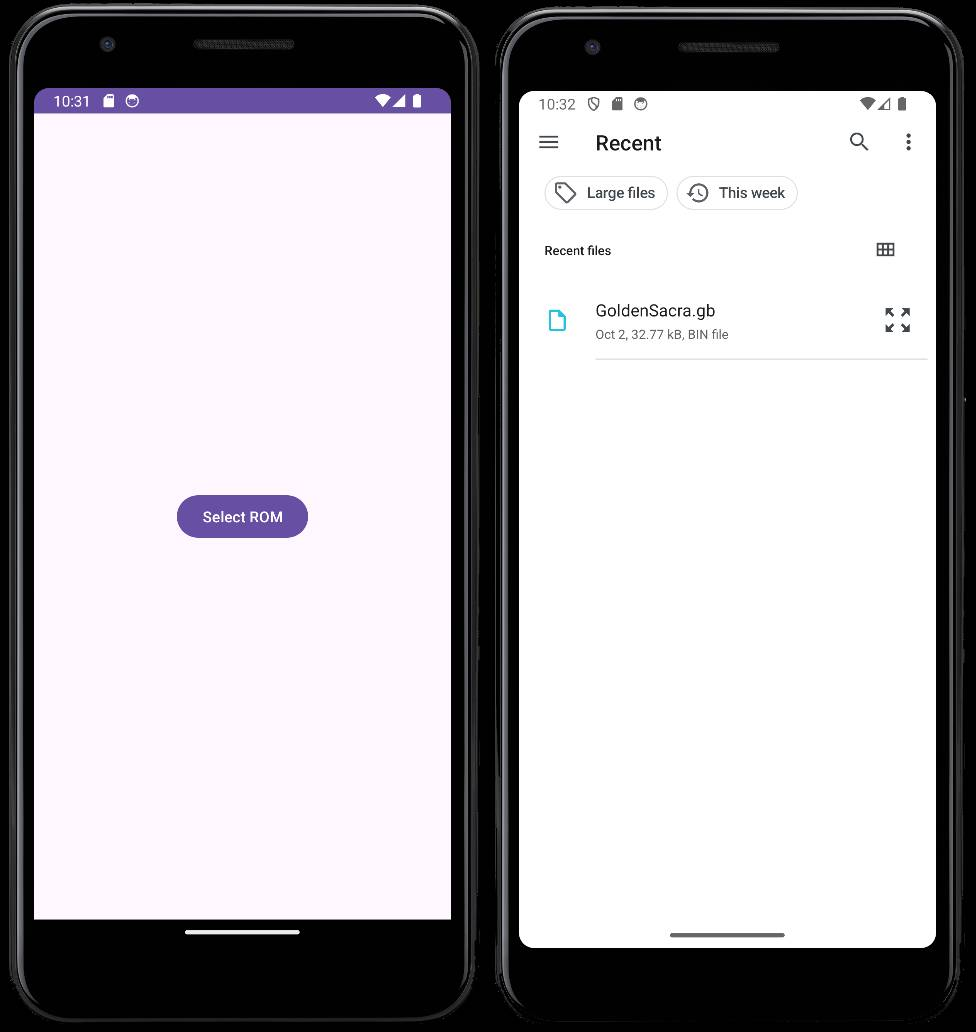
\includegraphics[width=0.4\textwidth]{include/images/openfile.jpg}
\caption{Selección de archivo desde la memoria SD del dispositivo.}
\label{figure:sdopen}
\end{figure}

A continuación, se procede a obtener los bytes del archivo y se envían al módulo de Emulator. En este momento, nos centraremos únicamente en la parte correspondiente a la ROM:

\begin{lstlisting}[language=Kotlin, caption={Carga de ROM y manejo de errores durante el proceso.}, label={code:kotlinloadrom}]
    fun load_rom(romBytes: ByteArray): Boolean{

        try {
            if(romBytes.isNotEmpty()){
                val cartSize = min(romBytes.size, ROM_END - ROM_START + 1)

                for (i in 0 until cartSize) {
                    Memory.write(ROM_START + i, romBytes[i])
                }

                return rom_init(romBytes)
            }
        }catch (ex: Exception){
            println("Error loading ROM: $ex")
        }

        return false
    }
\end{lstlisting}

En la función, se comprueba que los bytes pasados como parámetro no sean nulos. A continuación, se calcula el tamaño total de la ROM para asegurar que no exceda el tamaño máximo permitido (rango de 0x0000 a 0x7FFF). Se escriben todos los bytes en la memoria del emulador, y se invoca la función \textit{rom\_init()} para obtener datos como el título. Si alguna de las operaciones anteriores falla, se devuelve false y la ejecución se detiene.

\begin{lstlisting}[language=Kotlin, caption={Carga de ROM y manejo de errores durante el proceso.}, label={code:kotlinloadromread}]
    enum class CONSOLE_TYPE(val value : Int){
        DMG(0),
        DMG_CGB(0x80),
        CGB(0xC0),
        UNKNOWN(-1);

        companion object {
            fun fromValue(value: Int): CONSOLE_TYPE {
                return entries.find { it.value == value } ?: UNKNOWN
            }
        }
    }
    
    private var bootSection = ByteArray(0xFF)

    private var cartTitle : String      = "Unknown"
    private var licenseCode : String    = "None"
    private var cartType : Int          = -1
    private var romSize : Int           = -1
    private var ramSize : Int           = -1
    private var romVersion : Int        = -1
    private var console: CONSOLE_TYPE   = CONSOLE_TYPE.UNKNOWN

    [...]

    val newLicenseCodes: Map<String, String> = mapOf(
        "00" to "None",
        "01" to "Nintendo R&D1",
        "08" to "Capcom",
        "13" to "Electronic Arts",
        [...]
        "A4" to "Konami (Yu-Gi-Oh!)",
    )

    val oldLicenseCodes : Map<Int, String> = mapOf(
        0x00 to "None",
        0x01 to "Nintendo",
        0x08 to "Capcom",
        0x09 to "HOT-B",
        [...]
        0xFF to "LJN"
    )

    val cartTypes : Map<Int, String> = mapOf(
        0x00 to "ROM ONLY",
        0x01 to "MBC1",
        0x02 to "MBC1+RAM",
        0x03 to "MBC1+RAM+BATTERY",
        0x05 to "MBC2",
        [...]
        0xFF to "HuC1+RAM+BATTERY"
    )

    val ramSizes : Map<Int, Int> = mapOf(
        0x00 to 0, // KiB
        0x01 to 2,
        0x02 to 8,
        0x03 to 32,
        0x04 to 128,
        0x05 to 64
    )

    [...]

    fun convertBytesToString(bytes: ByteArray): String {
        val title = bytes.takeWhile { it != 0.toByte() && it.toInt() in 32..126 } // Filter only ASCII characters
        return String(title.toByteArray(), Charsets.US_ASCII)
    }

    fun rom_init(romBytes: ByteArray): Boolean{

        // Compare Cartridge Header with the Boot fixed one

        // Get header section from the romBytes
        val bootByteArray = Memory.getNintendoLogo()
        val cartByteArray = extractByteArray(romBytes, N_LOGO_START, N_LOGO_END, true) // Nintendo Logo on Cartridge goes from 0x104 to 0x133

        if(memcmp(Memory.getNintendoLogo(), cartByteArray, bootByteArray.size) != 0){
            return false
        }

        cartTitle   = convertBytesToString(extractByteArray(romBytes, TITLE_START, TITLE_END, true))

        licenseCode = if((extractByte(romBytes, OLD_LCNS_CODE).toInt() and 0xFF) == NEW_LICENSE_CODE){
            getNewLicenseNameFromIndex(convertBytesToString(extractByteArray(romBytes, LCNS_CODE_START, LCNS_CODE_END, true)))
        }else{
            getOldLicenseNameFromIndex(extractByte(romBytes, OLD_LCNS_CODE).toInt() and 0xFF)
        }

        cartType    = extractByte(romBytes, CART_TYPE).toInt() and 0xFF
        romSize     = 32 * (1 shl extractByte(romBytes, ROM_SIZE).toInt() and 0xFF) // Value in KiB
        ramSize     = extractByte(romBytes, RAM_SIZE).toInt() and 0xFF
        romVersion  = extractByte(romBytes, ROM_V_NUM).toInt() and 0xFF
        console     = CONSOLE_TYPE.fromValue(extractByte(romBytes, TITLE_END).toInt() and 0xFF)

        println("ROM Loaded Successfully!")

        bootSection = extractByteArray(romBytes, 0x00, 0xFF, true) // Save portion of code where the boot is going to load

        return true
    }
\end{lstlisting}

Desglosemos el código:

\begin{enumerate}
    \item Se compara el logotipo de Nintendo almacenado en el módulo de memoria con el presente en el cartucho. Si no coinciden, se procede a finalizar la ejecución del programa.
    \item Se obtienen los bytes correspondientes al título del juego y se convierten a una cadena de texto utilizando el conjunto de caracteres ASCII. Dado que la longitud del título depende de la versión del cartucho, se detendrá la lectura al encontrar el primer valor 0x00.
    \item Se extrae el código de licencia. Primero, se verifica si el valor antiguo contiene 0x33 para utilizar los nuevos códigos de licencia. De lo contrario, se empleará el listado antiguo. Ambos listados pueden definirse mediante un par de mapas (\textit{Maps}) para acceder rápidamente al valor correspondiente según el código obtenido.
    \item A continuación, se extraen de manera directa los valores correspondientes al tipo de cartucho, tamaño de la ROM/RAM, versión de la ROM y el tipo de mapper.
    \item Se realiza una copia de la región 0x0000-0x00FF del cartucho. La Game Boy "oculta" esta porción de código hasta que la secuencia de arranque ha finalizado.
\end{enumerate}

Aquí los resultados obtenidos con la carga de las ROMS \textit{Super Marioland}, \textit{Pokémon Azul} y \textit{Harry Potter y la Piedra Filosofal}:

\begin{lstlisting}[language=Consola, caption={Valores obtenidos tras la carga de ROM.}, label={code:romresults}]
--- Super Marioland
Cart Title: SUPER MARIOLAND
License: Nintendo
Cart Type: MBC1
ROM Size: 64
ROM Version Number: 0
RAM Size: 0
Console Type: DMG

--- Pokemon Azul
Cart Title: POKEMON BLUE
License: Nintendo R&D1
Cart Type: MBC5+RAM+BATTERY
ROM Size: 1024
ROM Version Number: 0
RAM Size: 3
Console Type: DMG

--- Harry Potter y la Piedra Filosofal
Cart Title: HARRYPOTTERBHVE
License: EA (Electronic Arts)
Cart Type: MBC5+RAM+BATTERY
ROM Size: 4096
ROM Version Number: 0
RAM Size: 2
Console Type: CGB
\end{lstlisting}

Además, se puede observar que la ROM se ha cargado correctamente en nuestra memoria virtual. En el caso de \textit{Harry Potter} y la piedra filosofal, los siguientes bytes son visibles en la región 0x0000-0x015F:

\begin{lstlisting}[language=Consola, caption={Visualización de la ROM cargada en la memoria virtual.}, label={code:rommemloaded}]
0000: E1 CD 9D 31 E9 87 87 87 85 6F 3E 00 8C 67 7E C9  | ...1.....o>..g~.
0010: 7A BC C0 7B BD C9 FF FF 3E 01 E0 A6 C9 FF FF FF  | z..{....>.......
0020: AF E0 A6 3E 02 E0 A8 C9 7C E0 51 7D E0 52 7A E0  | ...>....|.Q}.Rz.
0030: 53 7B E0 54 79 E0 55 C9 40 F5 D1 7B EA BA CD C9  | S{.Ty.U.@..{....
0040: C3 80 36 FF FF FF FF FF C3 CE C0 C3 AC 23 FF FF  | ..6..........#..
0050: FB C3 AC 39 FF FF FF FF C3 A3 38 FF FF FF FF FF  | ...9......8.....
0060: D9 D7 38 04 D5 54 5D E1 CB 2A CB 1B CB 2A CB 1B  | ..8..T]..*...*..
0070: CB 2A CB 1B 19 19 19 C9 CB 7C C8 F5 7D 2F C6 01  | .*.......|..}/..
0080: 6F 7C 2F CE 00 67 F1 C9 F5 79 2F C6 01 4F 78 2F  | o|/..g...y/..Ox/
0090: CE 00 47 F1 C9 CB 7A C8 F5 7B 2F C6 01 5F 7A 2F  | ..G...z..{/.._z/
00A0: CE 00 57 F1 C9 C5 06 08 AF 87 CB 15 30 04 84 30  | ..W.........0..0
00B0: 01 2C 05 20 F4 65 6F C1 C9 AF B5 20 03 65 37 C9  | .,. .eo.... .e7.
00C0: C5 D5 06 08 4D 2E 00 CB 14 CB 15 5D 7D 91 6F 3F  | ....M......]}.o?
00D0: 38 01 6B 05 20 F1 CB 14 B7 D1 C1 C9 C5 4D 44 3E  | 8.k. ........MD>
00E0: 0F 21 00 00 CB 23 CB 12 30 01 09 29 3D 20 F5 CB  | .!...#..0..)= ..
00F0: 7A 28 01 09 C1 C9 19 3E 02 EA 00 20 5E 23 56 C9  | z(.....>... ^#V.
0100: 00 C3 50 01 CE ED 66 66 CC 0D 00 0B 03 73 00 83  | ..P...ff.....s..
0110: 00 0C 00 0D 00 08 11 1F 88 89 00 0E DC CC 6E E6  | ..............n.
0120: DD DD D9 99 BB BB 67 63 6E 0E EC CC DD DC 99 9F  | ......gcn.......
0130: BB B9 33 3E 48 41 52 52 59 50 4F 54 54 45 52 42  | ..3>HARRYPOTTERB
0140: 48 56 45 C0 36 39 00 1B 07 02 01 33 00 D7 B4 78  | HVE.69.....3...x
0150: A7 FE 11 3E 00 20 01 3C E0 EF 31 FF CF F0 EF B7  | ...>. .<..1.....
\end{lstlisting}

\subsection{Lectura/Escritura en ROM}\label{rom:read_write}

\paragraph{Implementación de las Acciones de Lectura y Escritura en ROM}
Para implementar las operaciones, es necesario tener en cuenta cómo cada \hyperref[history_mbcs]{MBC} gestiona de manera específica las diferentes regiones de memoria y los registros asociados. Cada MBC presenta un mecanismo particular para el acceso y la selección de bancos de ROM y RAM, lo que afecta directamente la forma en que el emulador debe interactuar con ellos.
\\\\
Con el objetivo de lograr un emulador completo, es imprescindible implementar todos los tipos de controladores, desde el MBC1 hasta el MBC7, así como otros controladores especiales. No obstante, en este apartado se detallará exclusivamente la implementación del MBC1, que abarca una amplia gama de títulos, incluyendo juegos como \textit{Tetris DX} y \textit{Mario \& Yoshi}.
\\\\
La estructura propuesta, de forma que se faciliten la integración de los distintos tipos de MBC, es la siguiente:
\begin{itemize}
    \item Se generará una interfaz llamada MBCInterface, el cual tendrá dos funciones a implementar de lectura y escritura.
    \item Una clase abstracta MBC la cual implementa la interfaz y que contendrá datos como el modo de banca, el banco actual de ROM o los bancos de RAM.
    \item El módulo de ROM contendrá una variable de clase de tipo MBCInterface que por defecto será nulo y que obtendrá valor en la lectura inicial de ROM.
    \item El tipo NoMBC implementará directamente el MBCInterface, mientras que MBC1 heredará de la clase abstracta MBC.
    \item A la hora de escribir o leer en ROM, simplemente se trasladará la responsabilidad de la tarea a la variable guardada.
\end{itemize}

\begin{lstlisting}[language=Kotlin, caption={Inicialización del MBC.}, label={code:initmbc}]
    private var mbcInterface: MBCInterface?     = null
    [...]
    private fun initMBC(romBytes: ByteArray){
        mbcInterface = when(getCartTypeIndex()){
            0 -> NoMBC(romBytes)
            1 -> MBC1(romBytes)
            [...] // Resto de controladores
            else -> null
        }
    }   
\end{lstlisting}

Como ya ha sido explicado, dependiendo de las regiones de memoria en las que se intente escribir, se deben actualizar unos registros específicos.

\begin{lstlisting}[language=Kotlin, caption={Lectura en regiones ROM.}, label={code:romreadkotlin}]
    override fun read(address: Int): Byte {
        when (address) {
            in ROM_START..< ROM_SW_START -> { // READ FROM ROM FIXED BANK
                return when(bankingMode){
                    BankingMode.MODE_0 -> Memory.read(address)
                    BankingMode.MODE_1 -> romData?.get(getROM0BankAddr(address)) ?: 0xFF.toByte()
                }
            }
            in ROM_SW_START..ROM_END -> return romData?.get(getROMSwBankAddr(address)) ?: 0xFF.toByte() // READ FROM SWITCHABLE ROM BANK
            in EXTERNAL_RAM_START..< WRAM_START -> { // READ FROM EXTERNAL RAM
                return if(ramEnabled) {
                    ramBanks!![currentRamBank][address - EXTERNAL_RAM_START]
                } else 0xFF.toByte()
            }
        }

        return 0xFF.toByte()
    }
\end{lstlisting}

Desglosemos el código:

\begin{itemize}
    \item Si la dirección de memoria a leer se encuentra en el rango \texttt{0x0000-0x3FFF} (ROM fija o estática), primero se comprobará el modo de banco. En el caso del modo básico, la lectura se redirigirá al módulo de memoria. Para el modo avanzado, la lectura se realizará directamente sobre los bytes cargados del fichero \texttt{.gb/.gbc}. La función \texttt{getROM0BankAddr(address: Int)} verifica la cantidad de bancos ROM que contiene el cartucho, aplicando, si es necesario, una máscara y utilizando el registro de dos bits de la región \texttt{0x4000-0x5FFF} de manera complementaria.

    \item Si la dirección se encuentra en la región de ROM dinámica, \texttt{0x4000-0x7FFF}, los datos se obtendrán directamente del fichero \texttt{.gb/.gbc}. La función \texttt{getROMSwBankAddr(address: Int)} implementará una lógica similar a la de \texttt{getROM0BankAddr}, con la diferencia de que, en este caso, se sumará el resultado de la multiplicación entre el número de banco ROM actual y el tamaño de un banco (16 KiB) a la dirección indicada.

    \item Si la dirección se encuentra dentro del rango de la RAM externa, se comprobará primero que esta esté activada, para proceder a leer los valores correspondientes de la variable de clase.
\end{itemize}

Veamos ahora la escritura:

\begin{lstlisting}[language=Kotlin, caption={Escritura en regiones ROM.}, label={code:romwritekotlin}]
    override fun write(address: Int, value: Byte) {
        val valueInt = value.toInt() and 0xFF

        when {
            address <= ENABLE_RAM_END -> {  // ENABLE RAM
                if(cartHasRam())
                    ramEnabled = valueInt and 0xF == 0xA
            }
            address in (ENABLE_RAM_END + 1)..ROM_BANK_NUMBER_END -> {                           // ROM BANK SELECTION
                var currentRomBank = valueInt and romBankMask
                if (currentRomBank == 0) currentRomBank += 1
            }
            address in (ROM_BANK_NUMBER_END + 1)..RAM_BANK_NUMBER_END -> {                      // RAM BANK SELECTION
                if (bankingMode == BankingMode.MODE_1 && saveNeeded) {
                    saveExRAMToFile()
                }
                currentRamBank = valueInt and 0b11
            }
            address in (RAM_BANK_NUMBER_END + 1)..RAM_BANK_MODE_END -> {                        // BANKING MODE
                bankingMode = if (valueInt and 0b1 != 0) BankingMode.MODE_1 else BankingMode.MODE_0

                if(bankingMode == BankingMode.MODE_1 && saveNeeded){
                    saveExRAMToFile()
                }
            }
            address in EXTERNAL_RAM_START..< WRAM_START -> {                                       // WRITE TO EXTERNAL RAM
                if(ramEnabled){
                    ramBanks!![currentRamBank][address - EXTERNAL_RAM_START] = value

                    if(cartHasBattery()) saveNeeded = true
                }
            }
        }
    }
\end{lstlisting}

Desglosemos nuevamente el código:

\begin{itemize}
    \item Si la dirección de memoria se encuentra en el rango \texttt{0x0000} hasta \texttt{0x1FFF}, se realiza la habilitación de RAM externa. 
    \begin{itemize}
        \item Si el cartucho incluye RAM, se habilita la RAM cuando los 4 bits inferiores del valor escrito (\texttt{value}) son iguales a \texttt{0xA}.
    \end{itemize}
    
    \item Si la dirección está en el rango desde \texttt{0x2000} hasta \texttt{0x3FFF}, se selecciona el banco de ROM.
    \begin{itemize}
        \item Se determina el banco de ROM actual utilizando una máscara \texttt{romBankMask} y aplicándola a \texttt{value}. 
        \item Si el banco resultante es el banco 0 (que está reservado), se ajusta el valor a 1 para evitar acceder a la ROM reservada.
    \end{itemize}
    
    \item Si la dirección está en el rango desde \texttt{0x4000} hasta \texttt{0x5FFF}, se selecciona el banco de RAM.
    \begin{itemize}
        \item Si el modo de banca está en básico y es necesario guardar el estado, se llama a la función \texttt{saveExRAMToFile()} para almacenar los datos en el archivo de RAM externa.
    \end{itemize}
    
    \item Si la dirección está en el rango desde \texttt{0x6000} hasta \texttt{0x7FFF}, se define el modo de banca.
    \begin{itemize}
        \item Se selecciona el modo 1 si el bit menos significativo es 1, y modo 0 en caso contrario.
        \item Si el modo seleccionado es el básico y se requiere guardar, se realiza nuevamente el guardado con \texttt{saveExRAMToFile()}.
    \end{itemize}
    
    \item Si la dirección cae en el rango de RAM externa, \texttt{0xA000} hasta \texttt{0xBFFF}, se realiza una escritura en la RAM externa.
    \begin{itemize}
        \item Si la RAM está habilitada, el valor se escribe en el banco de RAM actual, ajustando la dirección para obtener la posición correcta.
        \item Si el cartucho tiene batería, se establece un flag para indicar que se requiere guardar.
    \end{itemize}
\end{itemize}

Con esto ya tendríamos lo básico para que nuestro controlador funcione. Partiendo de este ejemplo, se deben implementar el resto de los tipos existentes para asegurar que cualquier juego funcione.

\section{Interrupciones}

Las interrupciones deben ser procesadas en todos los ciclos de CPU, justo antes de ejecutar la siguiente instrucción de ROM. En la siguiente implementación, se puede ver el inicio del método \texttt{tick()}:

\begin{lstlisting}[language=Kotlin, caption={Interrupciones en el método principal de la CPU.}, label={code:cpuhandleinterrupt}]
    fun tick(): Boolean{

        // Interrupciones
        if(!pendingEI){
            handleInterrupts()
        }else{
            pendingEI = false
            Interrupt.enableInterrupts(true)
        }

        [...]
\end{lstlisting}

El flag \textit{pendingEI} es una variable que se activa en el momento que un opcode EI es ejecutado. Como se explicó previamente, esta instrucción no habilita las interrupciones de forma inmediata, si no que toma efecto en el siguiente ciclo de ejecución.
\\\\
En el método \texttt{handleInterrupts()}, se va a comprobar que las interrupciones estén habilitadas y que se deba procesar al menos una. En caso de que ambas condiciones se cumplan, se delegará el trabajo al módulo específico de las interrupciones.
\\\\
La lógica principal del módulo es la siguiente:

\begin{lstlisting}[language=Kotlin, caption={Lógica principal del módulo Interrupt.}, label={code:interruptlogic}]
    fun flush(){
        val activeInterrupts = getPendingInterrupts()

        if ((activeInterrupts and InterruptType.VBLANK.getInterruptMask()) != 0)        return handleInterrupt(VBLANK_PTR, InterruptType.VBLANK)
        else if ((activeInterrupts and InterruptType.LCD_STAT.getInterruptMask()) != 0) return handleInterrupt(LCD_STAT_PTR, InterruptType.LCD_STAT)
        else if ((activeInterrupts and InterruptType.TIMER.getInterruptMask()) != 0)    return handleInterrupt(TIMER_PTR, InterruptType.TIMER)
        else if ((activeInterrupts and InterruptType.SERIAL.getInterruptMask()) != 0)   return handleInterrupt(SERIAL_PTR, InterruptType.SERIAL)
        else if ((activeInterrupts and InterruptType.JOYPAD.getInterruptMask()) != 0)   return handleInterrupt(JOYPAD_PTR, InterruptType.JOYPAD)
    }

    private fun handleInterrupt(address: Int, type: InterruptType){
        enableInterrupts(false)       // IME se deshabilita para prevenir que otras interrupciones se ejecuten

        // Desactivar interrupciones
        val bit = (type.getInterruptMask()).inv()
        val ifValue = (Memory.getByteOnAddress(IF).toInt() and 0xFF)
        set_IF(ifValue and bit)

        CPU.executeInterrupt(address)
    }
\end{lstlisting}

Primero se ejecuta la función \texttt{flush()}, la cual se encarga de verificar las interrupciones pendientes y, si se detecta alguna, manejarla de manera adecuada:

\begin{enumerate}
    \item Se obtienen las interrupciones activas mediante la función getPendingInterrupts(), que retorna una máscara de bits representando las interrupciones pendientes.
    \item Se evalúa si cada tipo de interrupción está activa utilizando operaciones AND en combinación con las máscaras de interrupción.
    \item Si se detecta una interrupción activa para el tipo VBLANK, se llama a la función \texttt{handleInterrupt()} con la dirección de interrupción (0x0040) y el tipo correspondiente, finalizando así la ejecución de flush. Para el resto de tipos se hace lo mismo, siguiente la prioridad de bit.
\end{enumerate}

Por otro lado, la función \texttt{handleInterrupt(address: Int, type: InterruptType)} gestiona el proceso de atender una interrupción específica, asegurándose de que no se produzcan interrupciones adicionales durante su ejecución.

\begin{enumerate}
    \item Se deshabilitan las interrupciones globalmente llamando a enableInterrupts(false). Esto evita que otras interrupciones se ejecuten mientras se atiende la actual.
    \item Se lee el valor actual del registro IF, se realiza una operación bit a bit and con la máscara invertida para desactivar el bit correspondiente a la interrupción actual, y se actualiza en memoria.
    \item Finalmente, se ejecuta la rutina de servicio de interrupción llamando al método \\
    \texttt{executeInterrupt(address)}. En este se desactiva el HALT de la CPU (en caso de que lo estuviese), se pushea PC al stack pointer, y se sobreescribe PC con la dirección obtenida por parámetro. 
\end{enumerate}

Lo que ocurra a continuación depende de la decisión que haya tomado el desarrollador del juego que se ejecute.

\section{Temporizadores / Timers}

La implementación debe simular el comportamiento de los \hyperref[history_timer]{temporizadores} en el hardware original. Para ello se comenzará declarando unas constantes que representen las direcciones de memoria reales y se generarán las funciones de lectura y escritura:

\begin{lstlisting}[language=Kotlin, caption={Lectura y escritura en registros de Timers.}, label={code:timerwriteread}]
    const val DIV   = 0xFF04 // Divider Register (16 bit Register, but only the upper 8 bit (0-7) are public to the developer)
    const val TIMA  = 0xFF05 // Timer Counter
    const val TMA   = 0xFF06 // Timer Module
    const val TAC   = 0xFF07 // Timer Control

    [...]

    fun readFromTimer(address: Int): Byte{
        when(address){
            DIV -> return ((div16 shr 8) and 0xFF).toByte()
            TIMA -> return Memory.read(TIMA)
            TMA -> return Memory.read(TMA)
            TAC -> return Memory.read(TAC)
        }

        return 0
    }

    fun writeToTimer(address: Int, value: Byte){
        when(address){
            DIV -> {
                div16 = (div16 and 0xFF00)
            }
            TIMA -> Memory.write(TIMA, value)
            TMA -> Memory.write(TMA, value)
            TAC -> Memory.write(TAC, value)
        }
    }
\end{lstlisting}

A la hora de interactuar con el registro DIV, es importante considerar que internamente consta de 16 bits, aunque externamente solo se exponen los 8 bits más altos. Para manejarlo, se utiliza una variable de clase llamada \textit{div16}, que se inicializa siempre en 0x0000.
\\\\
Cuando se realiza una operación de escritura en este registro, únicamente se reinician a 0 los 8 bits menos significativos, preservando el estado de los 8 bits más altos. Por otro lado, al leer el registro, solo se devuelven los 8 bits más altos del valor contenido.
\\\\
Por último, se debe implementar la función que actualice en cada ciclo de ejecución el temporizador. Los pasos que debe seguir son:

\begin{itemize}
    \item Comparar el valor actual de DIV y verificar si ha llegado el momento de incrementar el contador TIMA basado en el valor de TAC (registro de control del temporizador).
    \item Usar el valor de TAC para determinar la frecuencia de incremento de DIV. Dependiendo de los dos primeros bits de TAC, el temporizador se incrementará a una velocidad diferente (256, 4, 16 o 64 ciclos de máquina).
    \item Si TIMA llega a 0xFF, se recarga con el valor de TMA y se genera una interrupción de temporizador.
\end{itemize}

\begin{lstlisting}[language=Kotlin, caption={Lectura y escritura en registros de Timers.}, label={code:timertick}]
    fun tick(){
        val prevDIV = div16
        div16 += 1

        var timerUpdate = false
        val tacValue = Memory.read(TAC).toInt() and 0xFF

        when(tacValue and 0b11){
            0b00 -> timerUpdate = (prevDIV and (1 shl 9) != 0) && (div16 and (1 shl 9) == 0)
            0b01 -> timerUpdate = (prevDIV and (1 shl 3) != 0) && (div16 and (1 shl 3) == 0)
            0b10 -> timerUpdate = (prevDIV and (1 shl 5) != 0) && (div16 and (1 shl 5) == 0)
            0b11 -> timerUpdate = (prevDIV and (1 shl 7) != 0) && (div16 and (1 shl 7) == 0)
        }

        if(timerUpdate && (tacValue and (1 shl 2) != 0)){
            var timaValue = Memory.read(TIMA).toInt() and 0xFF
            timaValue++
            Memory.write(TIMA, timaValue.toByte())

            if(timaValue == 0xFF){
                Memory.write(TIMA, Memory.read(TMA))
                Interrupt.requestInterrupt(Interrupt.InterruptType.TIMER.getByteMask())
            }
        }
    }
\end{lstlisting}

\section{RAM}

En la Game Boy, el término RAM puede hacer referencia a distintas áreas de memoria: WRAM (Working RAM), HRAM (High RAM), VRAM (Video RAM) o la RAM externa presente en algunos cartuchos. Este módulo se centrará en la implementación de WRAM y HRAM, ya que la VRAM está estrechamente vinculada al funcionamiento del módulo PPU (Processing Pixel Unit), mientras que la RAM externa está gestionada por los controladores de memoria de los cartuchos \hyperref[history_mbcs]{(MBC, Memory Bank Controllers)}.
\\\\
La implementación de la \textbf{HRAM}, siendo esta un espacio fijo de memoria, se delegará directamente al módulo Memory, que ya se encarga de manejar lecturas y escrituras en memoria. Debido a la simplicidad de su gestión y a que no requiere lógica específica adicional, no se desarrollará un apartado independiente para explicar su implementación en esta documentación.

\subsection{WRAM}
La WRAM en modo DMG es fija y se maneja directamente, mientras que en modo CGB incluye un banco fijo y hasta siete bancos conmutables adicionales, permitiendo que la memoria sea más dinámica. Estos bancos se almacenan en un array (\textit{wramBanks}) y el banco activo se controla mediante la variable \textit{wramBank}. Las lecturas y escrituras en la WRAM consideran si se está accediendo a un banco conmutable o al espacio fijo, ajustando automáticamente la dirección de memoria según sea necesario.

\begin{lstlisting}[language=Kotlin, caption={Lectura y escritura en Work RAM.}, label={code:wramreadwrite}]
    private var wramBanks: Array<ByteArray> = Array(CGB_SW_BANKS) { ByteArray(ECHO_RAM_START - SWITCHABLE_WRAM_START) } // Not used if not in CGB mode
    private var wramBank = 0

    fun readFromWRAM(address: Int) : Byte{
        return if(!ROM.isCGB() || address < SWITCHABLE_WRAM_START){
            Memory.read(address)
        }else{
            wramBanks[wramBank][address - SWITCHABLE_WRAM_START]
        }
    }

    fun writeToWRAM(address: Int, value: Byte){
        if(!ROM.isCGB() || address < SWITCHABLE_WRAM_START){
            Memory.write(address, value)
        }else{
            wramBanks[wramBank][address - SWITCHABLE_WRAM_START] = value
        }
    }
\end{lstlisting}

\subsection{VRAM}

Al estar estrechamente vinculada al módulo de la PPU, será ahi donde declaremos la variable. Únicamente se llegará a utilizar en modo CGB, ya que de otra forma acudiremos al módulo de memoria. Su implementación no tiene mucho más misterio: debe tener las dimensiones correctas y, en caso de estar en modo CGB, obtener o escribir los valores en ella:

\begin{lstlisting}[language=Kotlin, caption={Lectura y escritura en Video RAM.}, label={code:vramreadwrite}]
    private var vRam : ByteArray = ByteArray((VRAM_END - VRAM_START) + 1)

    fun readFromVRAM(address: Int) : Byte{
        return if(!ROM.isCGB()){
            Memory.read(address)
        }else{
            vRam[address - VRAM_START]
        }
    }

    fun writeToVRAM(address: Int, value: Byte){
        if(!ROM.isCGB()){
            Memory.write(address, value)
        }else{
            vRam[address - VRAM_START] = value
        }
    }
\end{lstlisting}

\subsection{RAM Externa}

La RAM Externa, como se ha visto, reside en los cartuchos y es gestionada por los controladores de memoria. En este caso, se ha implementado un controlador MBC1, por lo que la RAM externa se manejará a través de él. La lectura y escritura en la RAM externa se delegan al controlador MBC1, que se encarga de gestionar los bancos de RAM y de redirigir las operaciones a la RAM externa.
\\\\
La implementación ya se ha proporcionado en el apartado de \hyperref[rom:read_write]{lectura y escritura en ROM}.

\section{DMA}

Como se ha descrito en el \hyperref[dma]{apartado teórico}, definiremos una función que inicie el proceso de DMA. Por ahora no será utilizada, ya que para ello antes se debe implementar la PPU.
\\\\
En esta función de inicio daremos por activado el proceso, calcularemos la dirección de memoria sobre la que comenzar a iterar, y desactivaremos todas las interrupciones para que otra no pueda interrumpir la ejecución.

\begin{lstlisting}[language=Kotlin, caption={Inicio del proceso DMA.}, label={code:dmainit}]
    private var active : Boolean = false
    private var offset : Int = 0
    private var startAddress : Int = 0
    private var startDelay : Byte = 0

    fun start(value: Byte){ // Value: Indica el rango (0xXX00 - 0xXX9F)
        active = true
        offset = 0
        startDelay = 2
        startAddress = (value.toInt() and 0xFF) shl 8   // Si el valor es 0xC0, la dirección será 0xC000
        Interrupt.enableInterrupts(false) // Deshabilitamos las interrupciones
    }
\end{lstlisting}

En el método \textit{tick()} comprobaremos si hay o no un delay para comenzar la ejecución. En caso negativo obtendremos la dirección de inicio a la que le sumaremos el offset actual, y copiaremos el byte desde la RAM a la OAM. Al terminar de copiar los 160 bytes, desactivaremos el proceso y reactivaremos las interrupciones para continuar con la ejecución normal.

\begin{lstlisting}[language=Kotlin, caption={Proceso DMA.}, label={code:dmaprocess}]
    fun tick(){
        if (active){
            if(startDelay.toInt() == 0){
                val address = startAddress + offset
                PPU.writeToOAM(address, startAddress, Memory.getByteOnAddress(address))
                offset++
                active = (offset and 0xFF) < TOTAL_BYTES_TO_COPY

                if(!active)
                    Interrupt.enableInterrupts(true)
            }else{
                startDelay--
            }
        }
    }
\end{lstlisting}

\section{PPU}

En la PPU debemos antes de nada definir bastantes objetos con los que luego podamos trabajar de forma eficiente:
\begin{itemize}
    \item Enumeradores para obtener los bits individuales del LCDC, LCD Status, modo de PPU, paletas de color seleccionadas y atributos de un sprite.
    \item Un mapa que represente las distintas paletas y sus códigos de color con los que podamos trabajar en Android.
    \item Todas las variables de clase que necesitemos, como el contador de sprites por línea de renderizado, array de bytes para la VRam y la OAM, frame actual, paleta de color seleccionada, etc\ldots
\end{itemize}

Una vez definidos todos estos objetos, podremos pasar a inicializar la PPU:

\begin{lstlisting}[language=Kotlin, caption={Inicialización de la PPU.}, label={code:ppuinit}]
    fun init() {
        Memory.write(LCD_STAT, 0x81.toByte())
        Memory.write(LCDC_ADDR, 0x91.toByte())
        Memory.write(SCY, 0)
        Memory.write(SCX, 0)
        Memory.write(LY_ADDR, 0)
        Memory.write(LYC_ADDR, 0)
        Memory.write(WY, 0)
        Memory.write(WX, 0)
        val consoleType = ROM.getConsole()

        if(consoleType == ROM.CONSOLE_TYPE.DMG || consoleType == ROM.CONSOLE_TYPE.DMG_CGB) {
            Memory.write(BGP, 0xFC.toByte())
            Memory.write(OBP0, 0xFF.toByte())
            Memory.write(OBP1, 0xFF.toByte())
        }else{
            //TODO - CGB
        }

        handleLCDC(0x91.toByte())
    }

    [...]

    private fun handleLCDC(value: Byte){
        // Bit 7
        ppuEnabled = LCDCObj.LCDC_ENABLE.get(value) != 0
        lcdEnabled = ppuEnabled
        // Bit 6
        winTilemapAddr = if(LCDCObj.WIN_TILEMAP.get(value) == 0) TM_1_START else TM_2_START
        // Bit 5
        enabledWindow = LCDCObj.WINDOW_ENABLE.get(value) != 0
        // Bit 4
        addrModeAddr = if(LCDCObj.ADDRESS_MODE.get(value) == 0) SIGNED_TILE_REGION else VRAM_START
        // Bit 3
        bgTilemapAddr = if(LCDCObj.BG_TILEMAP.get(value) == 0) TM_1_START else TM_2_START
        // Bit 2
        objSize = if(LCDCObj.OBJ_SIZE.get(value) == 0) 8 else 16
        // Bit 1
        objEnabled = LCDCObj.OBJ_ENABLE.get(value) != 0
        // Bit 0
        bgWinEnabled = LCDCObj.MASTER_ENABLE.get(value) != 0
    }
\end{lstlisting}

Primero se configura la pantalla LCD:

\begin{itemize}
    \item \textbf{LCD Status (\texttt{LCD\_STAT})}: Se escribe el valor $0x81$ (\texttt{10000001} en binario). Este valor activa la interrupción cuando la línea de escaneo coincide con el valor de \texttt{LYC} y asegura que la pantalla empiece en un estado adecuado.
    \item \textbf{LCD Control (\texttt{LCDC})}: Se escribe el valor $0x91$ (\texttt{10010001} en binario), que habilita la pantalla, permite el uso de sprites y selecciona un modo de dirección de tiles.
\end{itemize}

Ahora configuramos los registros de desplazamiento y posición:
\begin{itemize}
    \item \textbf{\texttt{SCY} y \texttt{SCX}}: Se establecen en $0$ para que la imagen de fondo no esté desplazada.
    \item \textbf{\texttt{LY} y \texttt{LYC}}: Se inician en $0$ para que la pantalla empiece desde la primera línea de escaneo.
    \item \textbf{\texttt{WY} y \texttt{WX}}: Controlan la posición de la ventana en pantalla, comenzando en $0$.
\end{itemize}

Configuramos la paleta de colores detectando el tipo de consola:
\begin{itemize}
    \item Si es modo DMG o en en modo compatibilidad (DMG\_CGB):
    \begin{itemize}
        \item \textbf{\texttt{BGP}} se establece en $0xFC$ (\texttt{11111100} en binario), configurando la paleta de colores del fondo.
        \item \textbf{\texttt{OBP0} y \texttt{OBP1}} se establecen en $0xFF$, dejando los sprites con su configuración predeterminada.
    \end{itemize}
    \item Para el modo CGB, aún falta implementar la configuración específica.
\end{itemize}

Finalmente, se llama a \texttt{handleLCDC(0x91)} para aplicar la configuración del registro \texttt{LCDC}
\\\\
Al igual que el DMA y la CPU, la PPU también dispondrá de su propio método \texttt{tick()}. En él, comprobaremos que la PPU esté activa y ejecutaremos el código de los distintos modos según venga indicado en el \texttt{LCD Stat}.

\begin{lstlisting}[language=Kotlin, caption={Lógica principal de la PPU.}, label={code:pputick}]
    fun tick(){
        if(moduleIsActive()) {
            lineTicks++
            val stat = Memory.getByteOnAddress(LCD_STAT)

            when (StatObj.PPU_MODE.get(stat)) {
                PPUMode.HBlank.number -> hBlankMode(stat)       // MODE 0
                PPUMode.VBlank.number -> vBlankMode(stat)       // MODE 1
                PPUMode.OAM.number -> oamMode(stat)             // MODE 2
                PPUMode.DRAW_LCD.number -> drawLCDMode(stat)    // MODE 3
            }
        }
    }
\end{lstlisting}

\subsection{Modo 0: H-Blank}

El proceso verifica si se ha alcanzado el número total de ciclos (LINE\_TOTAL\_TICKS) para la línea actual y, si es así, se actualiza el valor del registro LY. Si la línea actual ha alcanzado o superado la resolución vertical de la Game Boy (GB\_Y\_RESOLUTION), significa que la PPU ha terminado de procesar todas las líneas visibles y entra en el modo V-Blank. En este caso, el método actualiza el estado de LCD\_STAT para reflejar este cambio y solicita una interrupción de V-Blank. Además, incrementa el contador de fotogramas y llama a calculateFPS() para actualizar la métrica de rendimiento.
\\\\
Por otro lado, si LY no ha alcanzado este límite, significa que la PPU aún está dentro del proceso de renderizado de la pantalla y debe volver al modo OAM. En este caso, el método actualiza LCD\_STAT para reflejar este cambio y, si la interrupción de estado del LCD para OAM está habilitada, solicita la interrupción correspondiente. Finalmente, restablece lineTicks a cero para comenzar el procesamiento de la nueva línea.

\begin{lstlisting}[language=Kotlin, caption={Lógica del proceso de H-Blank.}, label={code:ppuhblank}]
    private fun hBlankMode(stat: Byte){
        if(lineTicks >= LINE_TOTAL_TICKS){
            increment_LY()

            val ly = (Memory.getByteOnAddress(LY_ADDR).toInt()) and 0xFF

            if(ly >= GB_Y_RESOLUTION){ // ENTER VBLANK MODE
                Memory.write(LCD_STAT, StatObj.PPU_MODE.set(stat, PPUMode.VBlank.number))

                Interrupt.requestInterrupt(Interrupt.InterruptType.VBLANK.getByteMask()) // ASK FOR VBLANK INTERRUPT

                if(StatObj.VBLANK_INTERRUPT.get(stat) != 0)
                    Interrupt.requestInterrupt(Interrupt.InterruptType.LCD_STAT.getByteMask()) // ASK FOR LCD STAT INTERRUPT IF LCD_STAT HAS THE VBLANK BIT ACTIVATED

                currentFrame++

                calculateFPS()

            }else{ // RETURN TO OAM MODE
                Memory.write(LCD_STAT, StatObj.PPU_MODE.set(stat, PPUMode.OAM.number))

                if(StatObj.OAM_INTERRUPT.get(stat) != 0)
                    Interrupt.requestInterrupt(Interrupt.InterruptType.LCD_STAT.getByteMask()) // ASK FOR LCD STAT INTERRUPT IF LCD_STAT HAS THE OAM BIT ACTIVATED
            }

            lineTicks = 0
        }
    }
\end{lstlisting}

\subsection{Modo 1: V-Blank}

El proceso verifica si se ha alcanzado el número total de ciclos para la línea actual y, si es así, incrementa el valor del registro LY. Luego, obtiene el valor actualizado y comprueba si ha alcanzado o superado el número total de líneas. Si esto ocurre, significa que el periodo de V-Blank ha finalizado y la PPU debe volver al modo OAM para comenzar el renderizado del siguiente cuadro.
\\\\
En este caso, el método actualiza el estado de LCD\_STAT para reflejar el cambio al modo OAM y restablece LY\_ADDR a 0, indicando el inicio de un nuevo fotograma. Además, si la interrupción de estado del LCD para OAM está habilitada, solicita la interrupción. Al igual que en H-Blank, lineTicks se restablece a cero para comenzar el procesamiento de la nueva línea.

\begin{lstlisting}[language=Kotlin, caption={Lógica del proceso de V-Blank.}, label={code:ppuvblank}]
    private fun vBlankMode(stat: Byte){
        if(lineTicks >= LINE_TOTAL_TICKS){
            increment_LY()

            val ly = (Memory.getByteOnAddress(LY_ADDR).toInt()) and 0xFF

            if(ly >= TOTAL_LINES){ // RETURN TO OAM MODE
                Memory.write(LCD_STAT, StatObj.PPU_MODE.set(stat, PPUMode.OAM.number))
                Memory.write(LY_ADDR, 0)

                if(StatObj.OAM_INTERRUPT.get(stat) != 0)
                    Interrupt.requestInterrupt(Interrupt.InterruptType.LCD_STAT.getByteMask()) // ASK FOR LCD STAT INTERRUPT IF LCD_STAT HAS THE OAM BIT ACTIVATED
            }

            lineTicks = 0
        }
    }
\end{lstlisting}

\subsection{Modo 2: OAM Scan}

Aquí gestionamos el modo OAM Scan, el cual se encarga de escanear los sprites visibles en la línea actual antes de proceder al renderizado.
\\\\
Si el contador lineTicks ha alcanzado el número de ciclos necesarios para el modo OAM, la PPU cambia al modo de dibujo (DRAW\_LCD), actualizando el estado de LCD\_STAT y reiniciando los parámetros del FIFO fetcher, que se encarga de obtener los píxeles a renderizar. Sin embargo, en el primer ciclo, se inicializa el conteo de sprites en la línea y se llama a loadLineSprites(), que carga los sprites visibles en la línea actual para que puedan ser procesados durante la fase de dibujo.

\begin{lstlisting}[language=Kotlin, caption={Lógica del proceso de OAM Scan.}, label={code:ppuoamscan}]
    private fun oamMode(stat: Byte){ // MODE 2
        if(lineTicks >= OAM_CYCLES){ // ENTER DRAWING PIXELS MODE
            Memory.write(LCD_STAT, StatObj.PPU_MODE.set(stat, PPUMode.DRAW_LCD.number))
            fifoFetcher.resetParams() // Reset FIFO Fetcher
        }else if(lineTicks == 1){ // Scanning -> Read OAM on the first tick
            lineSpriteCount = 0
            loadLineSprites()
        }
    }
\end{lstlisting}

El método \texttt{loadLineSprites()} se encarga de seleccionar y ordenar los sprites que deben renderizarse en la línea de escaneo actual de la pantalla. Esta función solo se ejecuta si los sprites están habilitados o si la consola es un modelo CGB, ya que en este último caso siempre se procesan los sprites.
\\\\
Primero, se obtiene la línea de escaneo actual, sumándole un desplazamiento para compensar la posición real de los sprites. Luego, se determina el tamaño de los sprites, que puede ser de 8 o 16 píxeles. A continuación, se inicializa el array \texttt{objsFetched} con valores nulos y se resetea el contador que indica el número de sprites obtenidos por línea. Por último, se recorre la memoria OAM en bloques de 4 bytes (siendo cada uno en orden: posición Y, posición X, índice de tile y atributos). Si se han alcanzado el número máximo de sprites por línea, el bucle se detiene.
\\\\
Para cada sprite, se verifican las coordenadas x e y para determinar si es visible en la línea actual. Si lo es, se almacena en el array \texttt{objsFetched}, incrementando el contador a posteriori. Finalmente, se ordena la lista de sprites por su posición x, asegurando que aquellos con menor x se rendericen primero.

\begin{lstlisting}[language=Kotlin, caption={Obtención de sprites en modo OAM Scan.}, label={code:ppuoamscansprites}]
    private fun loadLineSprites(){

        if(objEnabled || ROM.isCGB()) { // CGB Ignores this condition

            val currentY = (Memory.getByteOnAddress(LY_ADDR).toInt() and 0xFF) + OAM_Y_OFFSET
            val lcdc = Memory.getByteOnAddress(LCDC_ADDR)
            val objSize = LCDCObj.OBJ_SIZE.get(lcdc)
            val spriteHeight = if (objSize == 0) 8 else 16

            objsFetched.fill(null)
            lineSpriteCount = 0

            for (i in oamRam.indices step 4) {

                if (lineSpriteCount >= MAX_OBJ_PER_SCANLINE) {
                    break
                }

                val y = oamRam[i].toInt() and 0xFF
                val x = oamRam[i + 1].toInt() and 0xFF
                val tile = oamRam[i + 2]
                val flags = oamRam[i + 3]

                if (x == 0 || x >= (GB_X_RESOLUTION + OAM_X_OFFSET)) { // Sprite not visible
                    continue
                }

                if (y <= currentY && (y + spriteHeight) > currentY) { // Sprite on current line
                    objsFetched[lineSpriteCount] = OAMObj(y.toByte(), x.toByte(), tile, flags)
                    lineSpriteCount++
                }
            }

            objsFetched.sortBy { it?.x ?: Byte.MAX_VALUE} // Sort by X position
        }
    }
\end{lstlisting}

\subsection{Modo 3: Drawing Pixels}

\cleardoublepage
\chapter{Resultados}
\label{results}

\cleardoublepage
\chapter{Conclusiones}
\label{develop}

\nocite{*}
\bibliography{bibliografia/bibliografia}
\bibliographystyle{apacite}

\end{document}
